%=====================================================================
%  ENSAE — Stage d'application 2025-2026
%  Analysis and modelling of digital public procurement (BOAMP / Gigalis)
%  Entry file: main.tex   |   Compile: pdfLaTeX + BibTeX + pdfLaTeX x2
%=====================================================================
\documentclass[11pt,a4paper]{article}

% ---------- encoding, language ----------
\usepackage[T1]{fontenc}
\usepackage[utf8]{inputenc}
\usepackage[round,authoryear]{natbib}
\usepackage[french,english]{babel}   % English main; French available for the note de synthèse
\usepackage{lmodern}
\usepackage{microtype}

% ---------- page geometry ----------
\usepackage[left=2.5cm,right=2.5cm,top=2.6cm,bottom=2.6cm]{geometry}
\usepackage{fancyhdr}
\pagestyle{fancy}
\fancyhf{}
\fancyhead[L]{\footnotesize\itshape Digital public procurement: observable successors, survival, and text}
\fancyhead[R]{\footnotesize\thepage}
\renewcommand{\headrulewidth}{0.3pt}
\setlength{\headheight}{14pt}
\setlength{\parskip}{0.55em}
\setlength{\parindent}{0pt}

% ---------- maths, figures, tables ----------
\usepackage{amsmath,amssymb}
\usepackage{graphicx}
\usepackage{float}
\usepackage{xcolor}
\usepackage{booktabs}
\usepackage{longtable}
\usepackage{array}
\usepackage{calc}
\usepackage{tikz}
\usetikzlibrary{arrows.meta,positioning,shapes.geometric}
\usepackage[font=small,labelfont=bf,width=0.95\textwidth]{caption}

% pandoc helpers
\providecommand{\tightlist}{\setlength{\itemsep}{0pt}\setlength{\parskip}{0pt}}
\providecommand{\passthrough}[1]{#1}
\newcommand{\real}[1]{#1}

% ---------- bibliography ----------
\bibliographystyle{plainnat}
\setcitestyle{aysep={,}}

% ---------- links ----------
\usepackage[hidelinks,breaklinks=true]{hyperref}
\hypersetup{pdftitle={Analysis and modelling of digital public procurement using BOAMP data},
            pdfauthor={ENSAE applied internship}}

% ---------- administrative placeholders: EDIT THESE FOUR LINES ----------
\newcommand{\studentName}{\textbf{[SURNAME First name]}}
\newcommand{\hostCity}{[City]}
\newcommand{\supervisorName}{[First name SURNAME]}
\newcommand{\internshipDates}{[start date] to [end date]}
%-----------------------------------------------------------------------

\begin{document}
\hypersetup{pageanchor=false}

% ENSAE mandatory cover layout (annex 1 of the school instructions)
\thispagestyle{empty}
\begin{center}
\vspace*{0.2cm}

\noindent
\begin{minipage}[t]{0.48\textwidth}
\raggedright
\large \studentName
\end{minipage}
\hfill
\begin{minipage}[t]{0.48\textwidth}
\raggedleft
\large \textbf{ENSAE 2\textsuperscript{e} année}\\[2pt]
\normalsize \emph{Stage d'application}\\
\normalsize \emph{Année scolaire 2025--2026}
\end{minipage}

\vspace{3.2cm}

\fbox{%
\begin{minipage}{0.92\textwidth}
\vspace{0.9cm}
\centering
{\LARGE \bfseries Analysis and modelling of digital public procurement using BOAMP data\par}
\vspace{0.6cm}
{\large Constructing an observable successor, survival analysis,\\ and technology segmentation from procurement text\par}
\vspace{0.9cm}
\end{minipage}}

\vfill

\noindent
\begin{minipage}[b]{0.48\textwidth}
\raggedright
\textbf{Gigalis}\\
\hostCity
\end{minipage}
\hfill
\begin{minipage}[b]{0.48\textwidth}
\raggedleft
\textbf{Maître de stage :} \supervisorName\\
\internshipDates
\end{minipage}

\vspace{1.2cm}
{\footnotesize This report is written in English. The mandatory French synthesis note is included at the end of the document.\par}
\vspace{0.4cm}
\end{center}
\clearpage


\cleardoublepage
\hypersetup{pageanchor=true}
\pagenumbering{roman}
\tableofcontents
\clearpage

\section*{Executive summary}
\addcontentsline{toc}{section}{Executive summary}
\markboth{Executive summary}{}

\emph{This note is independent of the report and can be read on its own. It is written for a non-specialist reader.}



\subsection*{The setting}

Gigalis is the public-interest group for digital services in the Pays de la Loire region. Among other roles it acts as a central purchasing body: it negotiates pooled contracts --- cloud, cybersecurity, networks, artificial intelligence --- that local authorities and public institutions may use, but are never obliged to. The value of those contracts depends on when they are opened. Open one too early and it sits unused; open it too late and buyers have already run their own procurements. Hence the question put to this internship: using public data, can we anticipate when a digital purchasing need will reappear?

\subsection*{What we know}

French public procurement notices are published in the BOAMP, an official bulletin that is freely accessible. This internship processed \textbf{1.6 million notices} published between 2015 and 2025 and derived a study population of \textbf{3,800 reconstructed awarded procurement episodes} containing a digital CPV code in the Grand Ouest region.

One obstacle appeared immediately and shaped the entire project: \textbf{the BOAMP never records that one contract renews another}. There is therefore no list of renewals to learn from. The information had to be constructed: for each awarded contract, search the later notices published by the same buyer for the one that continues the same need, and accept the match only when the resemblance is strong. What the study measures is consequently an \textbf{``observable successor''} --- a later procurement that visibly takes over --- and not a legal renewal. The distinction is maintained throughout, because it changes what may legitimately be concluded.

\subsection*{What the models indicate}

On this basis, roughly \textbf{one episode in seven} shows an observable successor before the end of 2025. The probability that a successor becomes visible is estimated at \textbf{4.6 \% within twelve months} of award and \textbf{6.7 \% within twenty-four months}. Follow-up differs across award years, and Kaplan--Meier estimation explicitly accounts for right censoring when estimating these age-specific probabilities; no causal explanation is assigned to their numerical level.

The most useful result is not that average level but its shape over time: the probability \textbf{rises markedly between the third and fourth year} of a contract, which matches the usual duration of public framework agreements. That is the window where monitoring pays off.

Two comparative readings require different levels of caution. Across the Grand Ouest population, episodes in \textbf{CPV-35 security and surveillance equipment} show earlier observable successors; that contrast weakens within the same buyer, suggesting that part of it reflects which buyers procure CPV-35. \textbf{Framework agreements} also show successors earlier. The association remains positive after direct detectability adjustment and in the primary within-buyer analysis, although its magnitude attenuates.

The second contribution is of a different kind. Public contracts are classified under a European administrative vocabulary that is too coarse for business use: a single category mixes telephony, software and IT services. A model trained on \textbf{500 hand-annotated notices} learns to recover, from the wording of the contract object alone, an eight-family business segmentation --- cloud, cybersecurity, networks, infrastructure, business software, data, artificial intelligence, IT services. It is \textbf{substantially better than the official vocabulary} for that purpose, and the gap is measured with its uncertainty. Gigalis therefore gains a technology-level reading that did not exist in the source data.

\subsection*{What remains uncertain}

Three points must be stated plainly.

\textbf{The quality of the matches is not independently validated.} It was measured against a reference sample built for the project, and on a very small number of accepted links. The order of magnitude is encouraging; the uncertainty interval is wide. A review by a procurement specialist is the missing control; the protocol and the sample are ready.

\textbf{Absolute levels depend strongly on the rule chosen.} Depending on how demanding the matching rule is, the number of successors identified ranges from 296 to 1,332. Percentages must therefore never be quoted alone. Several comparative patterns are more stable under changes to the event definition, but buyer-level composition matters: CPV-35 attenuates within buyer, framework magnitude weakens under controls, and a slower CPV-48 pattern appears only in the within-buyer sensitivity.

\textbf{Contract-by-contract prediction was not established.} A model was trained on the earlier years and tested on the recent ones without any refitting: its point estimate was close to chance, and the available temporal validation did not establish useful individual discrimination. The model is therefore not used as an individual ranking engine, and the ``twenty contracts most likely to be renewed'' table planned at the outset was not delivered.

\subsection*{What this means for Gigalis}

The work delivers \textbf{an instrument for measurement and monitoring, not a prediction engine}.

In practice it can say which \emph{groups} of contracts are entering the period where a successor becomes likely --- by segment and by age --- and focus human attention on the three-to-four-year window, starting with the fastest-moving segments. It provides a technology segmentation of the regional portfolio that can be used to map activity. And it leaves behind a reproducible, documented and tested pipeline that can be re-run on updated data.

As it stands, it does not support claiming that a specific contract will be renewed, nor forecasting the evolution of a segment: over the observed period, no volume trend survives the appropriate statistical tests.

\subsection*{What we recommend next}

\begin{enumerate}
\def\labelenumi{\arabic{enumi}.}
\tightlist
\item
  Have a sample of matches reviewed by an independent specialist before any quantified claim about the method's accuracy is communicated.
\item
  Have part of the technology corpus annotated by a second person, so that label reliability can be measured.
\item
  Provide Gigalis-internal membership data so that the causal question --- does opening a pooled contract actually change members' purchasing behaviour? --- can be addressed, which public data alone cannot do.
\item
  Treat individual prediction as a separate experiment, with its variables, validation protocol and success criterion fixed in advance, rather than as an adjustment of the current model.
\end{enumerate}

\clearpage

\cleardoublepage
\pagenumbering{arabic}

\section{Introduction}

Gigalis is the public-interest group responsible for digital services in the Pays de la Loire region. Among its roles it acts as a central purchasing body: it builds pooled framework agreements in cloud, cybersecurity, networks and artificial intelligence, which its members may use but are never obliged to. The strategic value of those agreements therefore depends on Gigalis anticipating its members' purchasing needs rather than observing them after the fact. The question put to this internship was: using historical data on digital public procurement, can we estimate the probability that a contract or a technology segment generates an identifiable purchasing need within the next twelve to twenty-four months?

The work was carried out entirely on open data --- the notices published in the \emph{Bulletin officiel des annonces des marchés publics} (BOAMP), 1,620,712 of them between 2015 and 2025, reduced to a study cohort of 3,800 awarded digital procurements in the Grand Ouest. The means were those of a standard workstation: Python, scikit-learn, lifelines, statsmodels and ruptures, with an end-to-end reproducible pipeline.

It became clear early on that the main difficulty was not estimating a duration but defining what is being measured. The BOAMP carries no field indicating that one contract renews another. The outcome variable therefore had to be constructed, and that construction governs everything downstream. This report presents the construction, the survival analysis it enables, the technology segmentation learnt from the text of the notices, the descriptive trend analysis, and a critical reading of what these results support --- and of what they do not.

\section{Context and reformulation of the problem}

\subsection{The business problem}

A central purchasing body pools demand. Its value is twofold: lower prices through volume, and one procedure instead of many. Both depend on opening the right framework agreement at the right time. Open one too early and it ties up a contract nobody uses; open it too late and members have already run their own procurements. The operational question is therefore a question about timing: when will a need that has already been met reappear?

The internship brief decomposed that question into three sub-problems, each attached to a family of methods: the lifetime problem (survival analysis), the trend problem (change-point detection in time series), and the text-signal problem (natural language processing). A fourth, causal dimension was mentioned as a research perspective if time allowed.

\subsection{What the BOAMP contains, and what it does not}

The BOAMP publishes notices: calls for competition, corrections, award notices. It does not publish contracts, and above all it publishes \textbf{no renewal identifier}. Nothing indicates that a contract awarded in 2023 replaces one awarded in 2019. There is therefore no ground truth for the event the brief called ``renewal''.

This is not a data-quality detail: it makes it impossible to pose the problem in its apparently natural form, ``estimate P(renewal within 12 months)'', because no renewal observation exists in the data from which to estimate anything. Two routes remain. The first is to \emph{assume} renewal --- for instance by declaring that a four-year framework agreement is renewed after four years. It was rejected: it would fabricate expiry dates for three quarters of the cohort, whose declared duration is missing (\S~3.4), and it would measure the assumption rather than the data. The second is to construct an observable and to own the gap between that observable and the legal concept. That is the route taken.

\subsection{The estimand: the observable successor}

\begin{quote}
\textbf{Definition.} An \emph{observable successor} of an awarded digital procurement is a later procurement episode, published in the BOAMP by the same buyer, that plausibly continues or replaces the same need, and that is \textbf{accepted} as such by a frozen, documented linkage rule.
\end{quote}

Three consequences follow, and the report carries them throughout.

First, the event is \emph{conditional on a rule}. Changing the rule changes the number of events: from 296 to 1,332 across the retained arms (\S~5.7). No absolute level can be quoted on its own.

Second, the event is \emph{observable}, not legal. A contract can be renewed without that being visible in the BOAMP --- through a central purchasing body, below publication thresholds, or through a successor the rule failed to recover. The absence of an accepted successor is \textbf{censoring}, never evidence of abandonment.

Third, linkage errors do not cancel out. A missed link removes an event and artificially extends a censored exposure; a false link fabricates both an event and its date. The two biases run in opposite directions, which forbids presenting the observed rate as a lower bound on the true re-procurement rate --- a point the record-linkage literature is explicit about \citep{doidge2019}.

\subsection{The questions as actually addressed}

\textbf{Q1.} Can an observable-successor variable of measurable quality be constructed from the BOAMP alone? (\S~4)
\textbf{Q2.} How long does it take for an awarded digital procurement to show an observable successor, and does that delay differ by segment and contract type? (\S~5)
\textbf{Q3.} Does the text of the notices carry a business technology segmentation that the administrative CPV vocabulary does not? (\S~6)
\textbf{Q4.} Does that learnt segmentation support readings the CPV segmentation cannot support? (\S~7)
\textbf{Q5.} Do quarterly volumes by segment show usable trends or breaks? (\S~8)
\textbf{Q6.} Does the model support individual, contract-level prediction? (\S~5.5 --- and the answer is no.)

\section{Data, units of analysis, and scope}

\subsection{Source and acquisition}

The source is the official BOAMP API \citep{boampapi}, operated by DILA and published on data.gouv.fr. Every notice published between 1 January 2015 and 31 December 2025 was downloaded in JSONL form and standardised by schema-aware parsers: raw values and parser lineage are preserved alongside normalised values, so that any cleaning decision remains traceable and reversible.

The extraction yields \textbf{1,620,712 unique notices}, with no duplicate identifier.

\subsection{From notice to episode: the first change of grain}

A notice is not a contract. The BOAMP republishes the same procedure several times --- call for competition, correction, award, sometimes lot by lot. Analysing at notice level would count the same procedure repeatedly and mechanically inflate any event rate.

Notices are therefore grouped into \textbf{procurement episodes} by connected-component search (union-find) over three edge types, in decreasing order of reliability:

\begin{enumerate}
\def\labelenumi{\arabic{enumi}.}
\tightlist
\item
  shared \texttt{contractFolderID} (45,885 edges accepted, 737 rejected for validated-buyer conflict);
\item
  explicit declared link between notices (584,896 edges);
\item
  identical procedure reference for the same buyer within a 730-day window (195,043 accepted, 861 rejected for exceeding the window).
\end{enumerate}

The result is \textbf{1,103,632 episodes}, 60.1 \% of them singletons. Reconstruction is an \emph{inference}, not an identifier supplied by the BOAMP; it is the first uncertainty the pipeline introduces, and it is measured: zero buyer-conflict episodes, zero impossible chronologies, every notice assigned to exactly one episode. 3,274 episodes carry more than one distinct procedure reference --- expected for multi-lot or republished procurements --- and are exported for inspection rather than silently corrected.

\subsection{The study cohort}

The selection funnel reconciles completely:

\begingroup\small
\begin{longtable}[]{@{}lr@{}}
\toprule\noalign{}
Step & Episodes \\
\midrule\noalign{}
\endhead
\bottomrule\noalign{}
\endlastfoot
Grand Ouest episodes & 144,269 \\
with at least one CPV code in divisions 32, 35, 48, 72 \citep{cpvreg2008} & 7,376 \\
carrying an award notice & 3,826 \\
with a resolvable award date & \textbf{3,800} \\
\end{longtable}
\endgroup

The 26 episodes lost at the last step have no usable award date and are dropped rather than dated by default.

\begin{figure}[htbp]
\centering
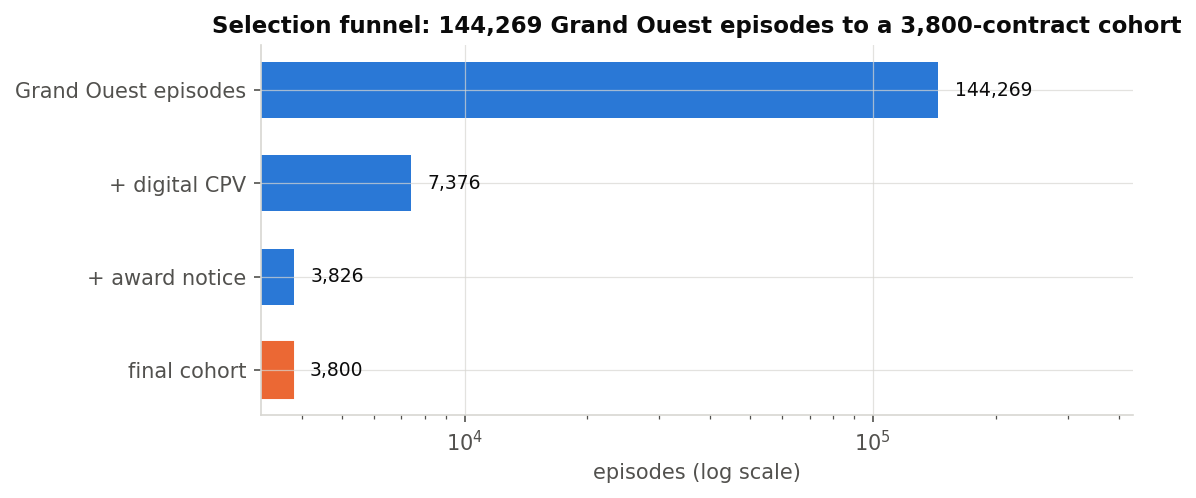
\includegraphics[width=0.95\linewidth]{figures/fig01_selection_funnel.png}
\caption{Selection funnel, from Grand Ouest episodes to the study cohort. Each bar is one criterion applied in order. \textbf{Note the logarithmic axis}: the first bar is 38 times the last, not four times as the relative lengths suggest. The 26 episodes lost at the final step have no resolvable award date and are dropped rather than dated by default.}
\label{fig:funnel}
\end{figure}


\textbf{One precision that matters.} The digital filter is an \textbf{any-code rule at episode level}: formally, episode \(e\) qualifies if \(\exists\, c \in \mathrm{CPV}(e)\) with \(\lfloor c/10^{6}\rfloor \in \{32,35,48,72\}\). It is not a rule about the main CPV. As a result, \textbf{1,176 of the 3,800 episodes (30.9 \%) have a main CPV outside those divisions}: multi-lot tenders that enter on a single digital lot. The cohort is therefore exactly ``awarded Grand Ouest procurement episodes containing at least one digital lot'', not ``3,800 digital procurements''. The first phrasing is used throughout.

The stratifying variable \texttt{digital\_segment} is the lowest-numbered digital division present, so each episode feeds exactly one curve. That tie-break is arbitrary and binds on the 412 episodes (10.8 \%) carrying more than one digital division. Its effect was measured rather than assumed: among the 2,624 episodes whose main CPV is itself digital, the assigned segment agrees with the main division 94.7 \% of the time, and event rates by assigned segment track those by main-CPV division closely (CPV-35: 0.2039 vs 0.1863; CPV-32: 0.1319 vs 0.1241). The rule is documented and kept.

Cohort composition: 1,452 episodes in Pays de la Loire, 1,282 in Normandie, 1,066 in Bretagne; 1,294 in CPV-72, 1,152 in CPV-32, 790 in CPV-48, 564 in CPV-35; median follow-up 2,015 days.

\subsection{Data quality and missing values}

\begingroup\small
\begin{longtable}[]{@{}
  >{\raggedright\arraybackslash}p{(\columnwidth - 6\tabcolsep) * \real{0.2308}}
  >{\raggedleft\arraybackslash}p{(\columnwidth - 6\tabcolsep) * \real{0.3077}}
  >{\raggedright\arraybackslash}p{(\columnwidth - 6\tabcolsep) * \real{0.2308}}
  >{\raggedright\arraybackslash}p{(\columnwidth - 6\tabcolsep) * \real{0.2308}}@{}}
\toprule\noalign{}
\begin{minipage}[b]{\linewidth}\raggedright
Field
\end{minipage} & \begin{minipage}[b]{\linewidth}\raggedleft
Missing
\end{minipage} & \begin{minipage}[b]{\linewidth}\raggedright
Decision
\end{minipage} & \begin{minipage}[b]{\linewidth}\raggedright
Reason
\end{minipage} \\
\midrule\noalign{}
\endhead
\bottomrule\noalign{}
\endlastfoot
Validated SIREN & 66.3 \% & Keep a name-only buyer key; audit risky links \citep{potin2023} & A SIREN identifies a legal unit \citep{insee_siren}; a similar name does not prove legal identity \\
Reliable duration & 74.9 \% & No imputation & Completeness moves from 11.8 \% in 2023 to 84.4 \% in 2025: missingness is not exchangeable over time \\
Amount container & 15.7 \% & Excluded from any monetary claim & The container holds several notice-level amount candidates with no validated canonical awarded value; comparable French award-notice datasets also require substantial consolidation \citep{potin2023} \\
Main CPV, text, award date & 0.0 \% & Required by selection & --- \\
\end{longtable}
\endgroup

Two of these decisions close routes the brief had envisaged and must be defended explicitly.

\textbf{Not imputing duration.} The brief proposed using declared duration to bound the renewal window (``a four-year contract is renewed within $\pm$6 months of its end''). That route was tested and then abandoned on evidence rather than convenience: among contracts holding both a reliable duration and an accepted successor, \textbf{only 21.8 \% are re-procured within six months of the declared end}, with a median absolute discrepancy of \textbf{21.1 months}. Declared duration is a poor predictor of the actual timetable. EU law itself treats four years as a general limit subject to justified exceptions \citep[Art.~33]{eudir2014}, not as the duration of every contract.

It is worth being precise about what ``excluding duration'' means, because the word misleads. Declared duration is
used \textbf{neither as a hard filter nor in the primary rule}: \texttt{M\_B} reads text alone. It does enter as \emph{graded
evidence} in the time component of \texttt{M\_C}'s weighted score, the contrast arm: where a reliable duration exists, the
component equals 1 at the declared end date and decays linearly to zero one year later; where it does not, the
component is \texttt{NaN} and drops out of both numerator \textbf{and} denominator rather than being scored zero. That is the
difference between ``I have no information'' and ``the information is unfavourable''. The project's initial design
substituted a four-year duration whenever the end date was unknown; that substitution was explicitly removed,
because it fabricated the single most influential timing input for most of the cohort.

\textbf{Not aggregating amounts.} No monetary analysis is produced. That is a real loss --- the brief expected amount series --- but a value reconstructed from an unvalidated container would produce series nobody could interpret.

\subsection{Scope decisions}

Two departures from the brief must be made explicit, because neither is neutral.

\textbf{Pays de la Loire $\rightarrow$ Grand Ouest.} The brief gave priority to Pays de la Loire, with extension to the Grand Ouest if volume proved insufficient. Volume alone did not force the extension: Pays de la Loire holds 1,452 episodes and 219 events, above the brief's own 800-contract minimum. What forces it is the \textbf{granularity} the research questions require:

\begingroup\footnotesize
\begin{longtable}[]{@{}
  >{\raggedright\arraybackslash}p{(\columnwidth - 10\tabcolsep) * \real{0.1364}}
  >{\raggedleft\arraybackslash}p{(\columnwidth - 10\tabcolsep) * \real{0.1818}}
  >{\raggedleft\arraybackslash}p{(\columnwidth - 10\tabcolsep) * \real{0.1818}}
  >{\raggedleft\arraybackslash}p{(\columnwidth - 10\tabcolsep) * \real{0.1818}}
  >{\raggedright\arraybackslash}p{(\columnwidth - 10\tabcolsep) * \real{0.1364}}
  >{\raggedleft\arraybackslash}p{(\columnwidth - 10\tabcolsep) * \real{0.1818}}@{}}
\toprule\noalign{}
\begin{minipage}[b]{\linewidth}\raggedright
Scope
\end{minipage} & \begin{minipage}[b]{\linewidth}\raggedleft
Episodes
\end{minipage} & \begin{minipage}[b]{\linewidth}\raggedleft
Events
\end{minipage} & \begin{minipage}[b]{\linewidth}\raggedleft
P(successor $\le$ 12 m)
\end{minipage} & \begin{minipage}[b]{\linewidth}\raggedright
95 \% CI
\end{minipage} & \begin{minipage}[b]{\linewidth}\raggedleft
Width
\end{minipage} \\
\midrule\noalign{}
\endhead
\bottomrule\noalign{}
\endlastfoot
Grand Ouest & 3,800 & 544 & 4.62 \% & {[}3.94; 5.30{]} & 1.37 pt \\
Pays de la Loire only & 1,452 & 219 & 5.36 \% & {[}4.17; 6.55{]} & 2.38 pt \\
\end{longtable}
\endgroup

The twelve-month interval is 1.7 times wider on Pays de la Loire alone; CPV-35 falls to 34 events there against 115 in Grand Ouest; and the larger scope provides materially stronger support for subgroup comparisons and for the downstream technology analyses. It also better matches the indicative study-size objective in the internship brief, which explicitly allowed extension beyond Pays de la Loire when needed. The extension is not neutral: region remains a model covariate, and aggregate results therefore read as ``Grand Ouest''.

\textbf{2015-2024 $\rightarrow$ 2015-2025.} The brief planned ten years to 2024. 2025 was kept, for two reasons and under one caveat. It is complete in volume: 93, 73, 73 and 87 episodes across the four quarters, against 72, 57, 72 and 85 in 2024; there is no publication gap before the 31 December 2025 cut-off. It adds 326 episodes of censored exposure that improve estimation at short horizons. But it is \textbf{incomplete in follow-up}: median follow-up for a 2025 award is 5.9 months against 59.9 months for 2015-2024, and the fourth quarter of 2025 can contain no event by construction. The effect is measurable: removing the 2025 awards moves the twelve-month estimate from 4.62 \% to 3.54 \%. 2025 is therefore kept, flagged as partial in follow-up, and \textbf{excluded from the primary temporal-validation window} (\S~5.5), where it appears only as a sensitivity read.

\subsection{Summary of grains}

\begin{figure}[htbp]
\centering
\footnotesize
\makebox[\linewidth][c]{%
\begin{tikzpicture}[
  node distance = 6mm and 12mm,
  box/.style   = {draw, rounded corners=2pt, align=center, inner sep=4pt,
                  minimum height=8mm, text width=52mm, fill=black!3},
  side/.style  = {align=left, text width=42mm, font=\scriptsize, text=black!65},
  flow/.style  = {-{Latex[length=2mm]}, thick, black!60},
  note/.style  = {draw, dashed, rounded corners=2pt, align=center, inner sep=4pt,
                  minimum height=8mm, text width=48mm, fill=black!2}
]

\node[box] (n1) {Official BOAMP notices};
\node[box, below=of n1] (n2) {Procurement episodes};
\node[box, below=of n2] (n3) {Study cohort};
\node[box, below=of n3] (n4) {Anchor--candidate pairs};
\node[box, below=of n4] (n5) {Accepted successor links};
\node[box, below=of n5] (n6) {Survival observations};

\draw[flow] (n1) -- node[right=1mm, font=\scriptsize] {schema-aware standardisation} (n2);
\draw[flow] (n2) -- node[right=1mm, font=\scriptsize] {Grand Ouest + digital CPV + awarded} (n3);
\draw[flow] (n3) -- node[right=1mm, font=\scriptsize] {same-buyer blocking, 90--2{,}920 days} (n4);
\draw[flow] (n4) -- node[right=1mm, font=\scriptsize] {\texttt{M\_B} top-1, accept at $0.70$} (n5);
\draw[flow] (n5) -- node[right=1mm, font=\scriptsize] {censor at 2025-12-31} (n6);

\node[side, left=of n1] {one official notice\\\textbf{1{,}620{,}712}};
\node[side, left=of n2] {one reconstructed procedure\\\textbf{1{,}103{,}632}};
\node[side, left=of n3] {one awarded digital episode\\\textbf{3{,}800}};
\node[side, left=of n4] {one pair to examine\\\textbf{763{,}417} over 3{,}520 anchors};
\node[side, left=of n5] {one accepted successor\\\textbf{544}};
\node[side, left=of n6] {one contract, event or censored\\\textbf{544} events, \textbf{3{,}256} censored};

\node[note, right=18mm of n6] (tech) {Predicted technology class\\for all 3{,}800 episodes\\\scriptsize (two quality gates before use)};
\draw[flow, dashed] (n3.east) -- ++(28mm,0) |- (tech.north);
\draw[flow, dashed] (tech.west) -- ++(-6mm,0) |- (n6.east);

\end{tikzpicture}}
\caption{The analytical chain, with the unit of observation at each stage. Every arrow is a change of
statistical unit, and each introduces uncertainty that propagates downstream. The dashed path is the
enrichment layer: the technology classifier reads the cohort's procurement text and returns a predicted class
that is joined back onto the survival table, without altering the cohort definition or the event.}
\label{fig:pipeline}
\end{figure}



\begingroup\small
\begin{longtable}[]{@{}
  >{\raggedright\arraybackslash}p{(\columnwidth - 4\tabcolsep) * \real{0.3000}}
  >{\raggedright\arraybackslash}p{(\columnwidth - 4\tabcolsep) * \real{0.3000}}
  >{\raggedleft\arraybackslash}p{(\columnwidth - 4\tabcolsep) * \real{0.4000}}@{}}
\toprule\noalign{}
\begin{minipage}[b]{\linewidth}\raggedright
Layer
\end{minipage} & \begin{minipage}[b]{\linewidth}\raggedright
One row represents
\end{minipage} & \begin{minipage}[b]{\linewidth}\raggedleft
Count
\end{minipage} \\
\midrule\noalign{}
\endhead
\bottomrule\noalign{}
\endlastfoot
Standardised notices & one official BOAMP notice & 1,620,712 \\
Episodes & one reconstructed procurement procedure & 1,103,632 \\
Study cohort & one awarded Grand Ouest digital episode & 3,800 \\
Candidate table & one anchor-candidate pair & 763,417 \\
Survival table & one cohort episode with an observed or censored time & 3,800 \\
\end{longtable}
\endgroup

Each arrow between these layers is a change of statistical unit, and each introduces uncertainty that propagates to the final results. That is why the report treats them as methodological objects rather than preparation steps.

\section{Constructing the outcome: successor linkage}

\subsection{Why this step exists}

Survival analysis needs two numbers per awarded procurement episode: a delay and an event indicator. The BOAMP supplies neither. This section builds both, and measures the quality of that construction --- because an error here is corrected nowhere downstream.

\subsection{Candidate generation}

For each \textbf{anchor} \(i\) (an awarded cohort episode with origin \(u_i\)), a later episode \(j\) with origin \(v_j\) is exposed for comparison if and only if:

\begin{itemize}
\tightlist
\item
  buyer identifiers are compatible --- same buyer key or same normalised name, with two different validated SIRENs disqualifying;
\item
  and the chronology satisfies
  \[u_i + 90\ \text{days} \le v_j \le u_i + 2{,}920\ \text{days}.\]
\end{itemize}

The 90-day to 8-year window is an \textbf{operational search range}, not an assumed contract duration. Git and notebook history place the 90-day floor in the candidate-generation notebook committed on 11 August 2026, before the final pipeline was frozen. It responded to a clear concurrent-procurement pathology: without a floor, \texttt{132} of the \texttt{628} links then accepted fell within three months of award, and every link for a 2025 award sat under twelve months, with a median of 1.7. The same design check also used the full reviewed successor set: the shortest of the 23 reviewed gaps was \textbf{139 days}, so the floor excluded none of them. Candidate generation was therefore informed by broader reference diagnostics, including the designated locked stratum; it was not evaluated as an untouched component. The eight-year ceiling likewise excludes no reviewed successor.

The result is \textbf{763,417 pairs} covering \textbf{3,520 of the 3,800 anchors}. The 280 anchors with no candidate at all stay in the analysis as censored exposure: their status is decided by blocking, not by the acceptance bar.

\textbf{No hard CPV filter, and the argument is empirical.} Requiring the successor to share the anchor's CPV division would be tempting. The reference forbids it: of the 23 reviewed successors, \textbf{9 (39.1 \%) cross a division}. Hard blocking would destroy them and cut the attainable recall ceiling from 0.913 to 0.609. The literature points the same way: CPV assignment is documented as error-prone even for experts \citep{siciliani2023}. CPV is therefore used as continuity evidence, never as a hard constraint.

\subsection{Four methods on the same pairs}

\begingroup\small
\begin{longtable}[]{@{}
  >{\raggedright\arraybackslash}p{(\columnwidth - 4\tabcolsep) * \real{0.3333}}
  >{\raggedright\arraybackslash}p{(\columnwidth - 4\tabcolsep) * \real{0.3333}}
  >{\raggedright\arraybackslash}p{(\columnwidth - 4\tabcolsep) * \real{0.3333}}@{}}
\toprule\noalign{}
\begin{minipage}[b]{\linewidth}\raggedright
M.
\end{minipage} & \begin{minipage}[b]{\linewidth}\raggedright
Role
\end{minipage} & \begin{minipage}[b]{\linewidth}\raggedright
Principle
\end{minipage} \\
\midrule\noalign{}
\endhead
\bottomrule\noalign{}
\endlastfoot
\texttt{M\_A\_deterministic} & Conservative comparator & Requires buyer, CPV and a minimum text-similarity floor \\
\texttt{M\_B\_text\_ranking} & \textbf{Primary method} & Takes the highest TF-IDF cosine candidate and accepts it above the threshold \\
\texttt{M\_C\_weighted\_gated} & High-recall comparator & Weighted score, buyer 0.50 / text 0.25 / CPV 0.20 / time 0.05, renormalised over observed evidence \\
\texttt{M\_D\_fellegi\_sunter} & Probabilistic comparator & Match / non-match likelihood ratios \citep{fellegi1969} \\
\end{longtable}
\endgroup

The primary decision rule is
\[\hat{j}_i = \arg\max_{j \in J_i} T_{ij}, \qquad Y_i = \mathbf{1}\!\left(T_{i\hat{j}_i} \ge 0.70\right),\]
where \(T_{ij}\) is the maximum of a word-level and a character-level TF-IDF cosine similarity. \textbf{At most one successor per anchor}; otherwise the method abstains.

One implementation detail has consequences analysed in \S~5.7: the vectoriser is fitted \emph{per anchor block}. That choice has a reason --- the IDF weights become local to the buyer's own vocabulary, which stops the administrative boilerplate common to all of a buyer's notices from dominating the similarity --- and it has a cost: the score becomes block-relative, a fixed 0.70 does not mean quite the same thing for every anchor, and the maximum over a larger block is mechanically higher. \S~5.7d measures that cost rather than assuming it negligible.

\subsection{Operating-point chronology and validation status}

The 0.70 threshold follows a precision-first principle: a false link fabricates both an event and its date, whereas a missed link does not fabricate an event. The project history nevertheless does \textbf{not} support calling its final reference result fully held out. An earlier committed linkage script records that the \texttt{M\_B @ 0.70} policy drew on inspection of the designated locked split; candidate-generation diagnostics also used the full reviewed successor set. The operating point was subsequently frozen and never moved, so the current sweep is a transparent \textbf{internal validation and sensitivity display}, not an untouched external test of every pipeline decision. The 0.60 arm is retained to show the precision--recall trade rather than promoted post hoc.

The brief anticipated a linkage rate of 40-60 \%. The realised rate is \textbf{14.3 \%}. This is not a shortfall against a target: the brief's figure was treated as a planning assumption, never as an optimisation objective, and 14.3 \% is the arithmetic consequence of a precision-first rule combined with an event defined as \emph{observable in the BOAMP}.

\begin{figure}[htbp]
\centering
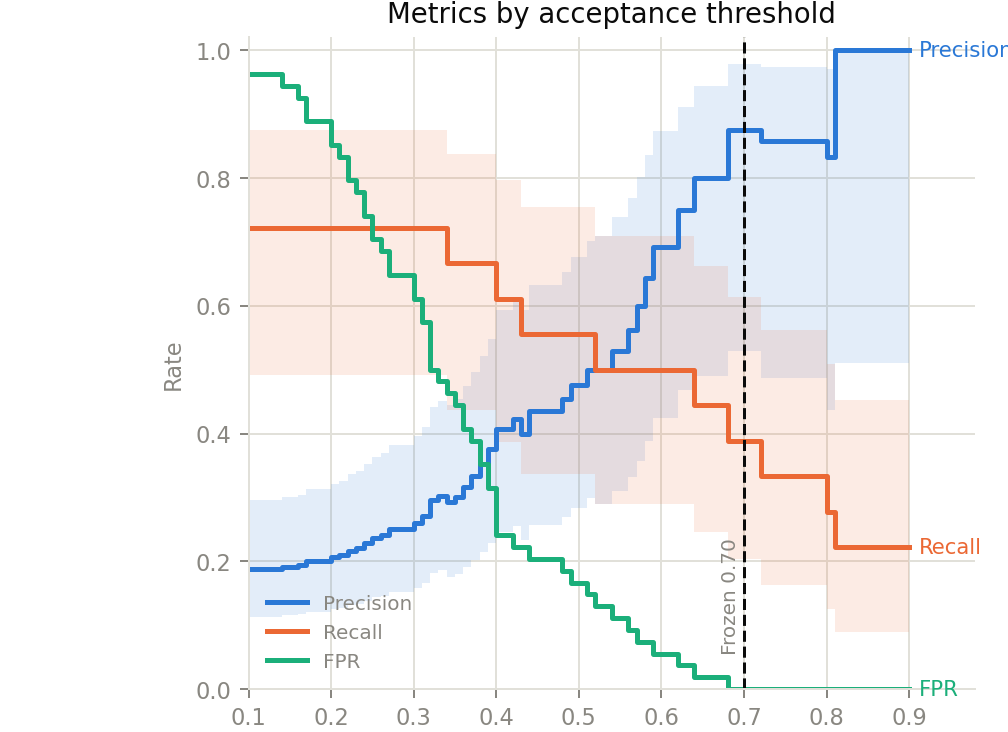
\includegraphics[width=0.78\linewidth]{figures/fig05_threshold_left_panel.png}
\caption{Precision, recall, false-positive rate and accepted-link volume as a function of the \texttt{M\_B} acceptance threshold on the reference stratum designated \texttt{LOCKED\_TEST}. The retained 0.70 operating point is marked. Project history shows that this evidence informed the final policy, so the panel is an internal-validation display rather than an untouched holdout. Shaded bands are 95\,\% Wilson intervals and every riser is one anchor changing decision, on 72 anchors of which 18 have a reviewed successor. The full three-panel version is Figure~\ref{fig:appc-tradeoff} in Annex C.}
\label{fig:threshold}
\end{figure}


\subsection{The regional reference, and what it is worth}

The evaluation strategy follows the three-part scheme recommended for linked data \citep{harron2017}: score the algorithm on a reference subset, compare linked with unlinked records, and test whether conclusions survive changes to the linkage procedure. Evaluation rests on a stratified review of \textbf{120 Grand Ouest anchors}, carried out on 11 August 2026 against the real BOAMP notices and their official URLs, \textbf{before the linkage methods in this project existed}. 112 anchors re-resolve onto exactly one episode and 88 are usable; the pilot (16 anchors) / locked (72 anchors) split is recorded in the reference file itself and is not post hoc.

Four limits bound its reach, and they belong in the body of the report rather than in a footnote:

\begin{enumerate}
\def\labelenumi{\arabic{enumi}.}
\tightlist
\item
  \textbf{The labels come from a single large-language-model research pass}, spot-checked by the project owner rather than verified anchor by anchor, and not judged by a specialist panel. They are independent of every method scored --- none existed at the time --- but they are not human ground truth.
\item
  \textbf{The per-anchor evidence trail was not recorded}: the sources behind a given decision cannot be reconstructed.
\item
  \textbf{Negatives are corpus-relative}: roughly 25 candidates per anchor were considered, not the full pool. A negative means ``no successor identified among those examined''.
\item
  \textbf{Candidate-surfacing independence does not hold.} The rule that selected those \textasciitilde25 candidates (from pools of up to 3,258) is recorded nowhere, and all 16 retrievable locked-split successors rank within the top thirteen by the very text score being evaluated. Consequently \textbf{recall and the 0.913 ceiling are not fully independent of the score they bound}. Precision is unaffected: a false positive is a false positive however the list was assembled.
\end{enumerate}

\subsection{Internal-validation results on the designated locked stratum}

Two accountings coexist and do not answer the same question. \emph{Anchor-level} accounting asks whether the system detected that a successor exists. \emph{Exact-successor} accounting, which is stricter, asks whether it named the right one; a wrong successor on a positive anchor then counts as one false positive \textbf{and} one false negative. The project's headline figures are the latter.

\begingroup\footnotesize
\begin{longtable}[]{@{}
  >{\raggedright\arraybackslash}p{(\columnwidth - 18\tabcolsep) * \real{0.0811}}
  >{\raggedright\arraybackslash}p{(\columnwidth - 18\tabcolsep) * \real{0.0811}}
  >{\raggedleft\arraybackslash}p{(\columnwidth - 18\tabcolsep) * \real{0.1081}}
  >{\raggedleft\arraybackslash}p{(\columnwidth - 18\tabcolsep) * \real{0.1081}}
  >{\raggedleft\arraybackslash}p{(\columnwidth - 18\tabcolsep) * \real{0.1081}}
  >{\raggedleft\arraybackslash}p{(\columnwidth - 18\tabcolsep) * \real{0.1081}}
  >{\raggedleft\arraybackslash}p{(\columnwidth - 18\tabcolsep) * \real{0.1081}}
  >{\raggedright\arraybackslash}p{(\columnwidth - 18\tabcolsep) * \real{0.0811}}
  >{\raggedleft\arraybackslash}p{(\columnwidth - 18\tabcolsep) * \real{0.1081}}
  >{\raggedleft\arraybackslash}p{(\columnwidth - 18\tabcolsep) * \real{0.1081}}@{}}
\toprule\noalign{}
\begin{minipage}[b]{\linewidth}\raggedright
M.
\end{minipage} & \begin{minipage}[b]{\linewidth}\raggedright
Thr.
\end{minipage} & \begin{minipage}[b]{\linewidth}\raggedleft
TP
\end{minipage} & \begin{minipage}[b]{\linewidth}\raggedleft
FP
\end{minipage} & \begin{minipage}[b]{\linewidth}\raggedleft
FN
\end{minipage} & \begin{minipage}[b]{\linewidth}\raggedleft
TN
\end{minipage} & \begin{minipage}[b]{\linewidth}\raggedleft
Precision
\end{minipage} & \begin{minipage}[b]{\linewidth}\raggedright
95 \% CI
\end{minipage} & \begin{minipage}[b]{\linewidth}\raggedleft
Recall
\end{minipage} & \begin{minipage}[b]{\linewidth}\raggedleft
FPR
\end{minipage} \\
\midrule\noalign{}
\endhead
\bottomrule\noalign{}
\endlastfoot
\texttt{M\_A} & n/a & 8 & 7 & 10 & 47 & 0.533 & 0.301-0.752 & 0.444 & 0.130 \\
\textbf{\texttt{M\_B}} & \textbf{0.70} & \textbf{7} & \textbf{1} & \textbf{11} & \textbf{54} & \textbf{0.875} & \textbf{0.529-0.978} & \textbf{0.389} & \textbf{0.000} \\
\texttt{M\_C} & 0.70 & 12 & 11 & 6 & 44 & 0.522 & 0.330-0.708 & 0.667 & 0.185 \\
\texttt{M\_D} & 0.65 & 1 & 4 & 17 & 53 & 0.200 & 0.036-0.625 & 0.056 & 0.018 \\
\end{longtable}
\endgroup

Three readings, in order of importance.

\textbf{The intervals overlap heavily.} A precision of 0.875 resting on \textbf{eight accepted links} has an interval running from ``coin flip'' to ``near perfect''. The figure must never be quoted without it, and this reference separates the methods only coarsely.

\textbf{Recall is capped before any scoring.} Candidate generation exposes only 21 of the 23 reviewed successors, a pairs completeness of 0.913 \citep{christen2007}; both unreachable cases are attributed to a named blocking condition --- one anchor never entered the cohort for want of a structured address, one buyer changed legal form from CCAS to CIAS with no shared SIREN. No unexplained case, which is what distinguishes an owned ceiling from an implementation defect.

\textbf{The precision-recall trade is deliberate.} \texttt{M\_C} buys recall (0.667) at half the precision (0.522). For survival analysis that is not a neutral exchange: its 11 false positives would introduce eleven events that never happened, with eleven dates that never happened.

\subsection{Challenge review and linkage audit}

A blinded 60-pair sample was prepared (20 production-accepted links, 20 high-similarity structural negatives, 20 buyer-declared relationships), with a separate audit key and a pre-specified acceptance rule. The review that was carried out is \textbf{model-assisted, not independent-human} --- its provenance is recorded explicitly in the repository. Of the 20 accepted links: 14 confirmed, 5 rejected, 1 uncertain, giving a precision of \textbf{0.700} on a conservative reading (95 \% CI {[}0.457; 0.881{]}), \textbf{below the 0.80 target} the project set itself.

The result is reported as it stands. It does not close the validation gate; it makes closing it necessary. Independent human review is the first recommendation in \S~9.F.

\subsection{What linkage produces}

\textbf{544 accepted links} over 3,800 anchors, an event rate of \textbf{14.32 \%}. CPV continuity: 351 of the 538 links with both divisions observed stay within one division (65.2 \%), comparable to the reviewed reference successors (14 of 23, 60.9 \%). 461 distinct successors for 544 links: 44 episodes are accepted by more than one anchor, the most reused by eleven --- a false-positive signature exploited in \S~5.7. Zero accepted links with conflicting validated SIRENs; zero municipality / inter-municipal mixes.

\section{Survival analysis}

\subsection{Time and censoring}

For an anchor \(i\) whose successor \(\hat{j}_i\) is accepted:
\[\tau_i = v_{\hat{j}_i} - u_i, \qquad Y_i = 1.\]
If no successor is accepted before 31 December 2025:
\[\tau_i = \text{2025-12-31} - u_i, \qquad Y_i = 0,\]
and the row is \textbf{administratively right-censored}. Time zero is the award date.

The cohort therefore holds \textbf{3,800 awarded procurement episodes, 544 events and 3,256 censored observations} (85.7 \%). That high censoring rate is precisely why survival analysis is used rather than a regression on linked episodes alone: ignoring censoring would restrict the analysis to episodes whose successor has been seen, that is, condition the analysis on the outcome.

\subsection{Non-parametric estimation}

The Kaplan--Meier estimator \citep{kaplan1958},
\[\hat S(t) = \prod_{t_k \le t}\left(1 - \frac{d_k}{n_k}\right),\]
with \(d_k\) events at \(t_k\) and \(n_k\) at risk, assumes no distributional form and handles administrative censoring without bias as long as censoring is independent of the hazard.

\begingroup\footnotesize
\begin{longtable}[]{@{}lrr@{}}
\toprule\noalign{}
Horizon & P(observable successor) & Survival \\
\midrule\noalign{}
\endhead
\bottomrule\noalign{}
\endlastfoot
12 months & \textbf{4.62 \%} & 0.9538 \\
24 months & \textbf{6.73 \%} & 0.9327 \\
36 months & 8.68 \% & 0.9132 \\
48 months & 15.50 \% & 0.8450 \\
60 months & 17.54 \% & 0.8246 \\
\end{longtable}
\endgroup

\textbf{The Kaplan-Meier median is not reached}: the curve never falls below 0.5 within the observation window. The 31.8 months quoted elsewhere is the median \emph{among linked events only}; the two quantities share a word and measure different things, the second being conditional on the event having occurred.

The jump between 36 and 48 months --- 8.7 \% to 15.5 \% --- is the \textbf{re-procurement shoulder}. Its timing is compatible with multi-year purchasing cycles, but the event is an observable successor and does not establish a legal renewal.

\begin{figure}[htbp]
\centering
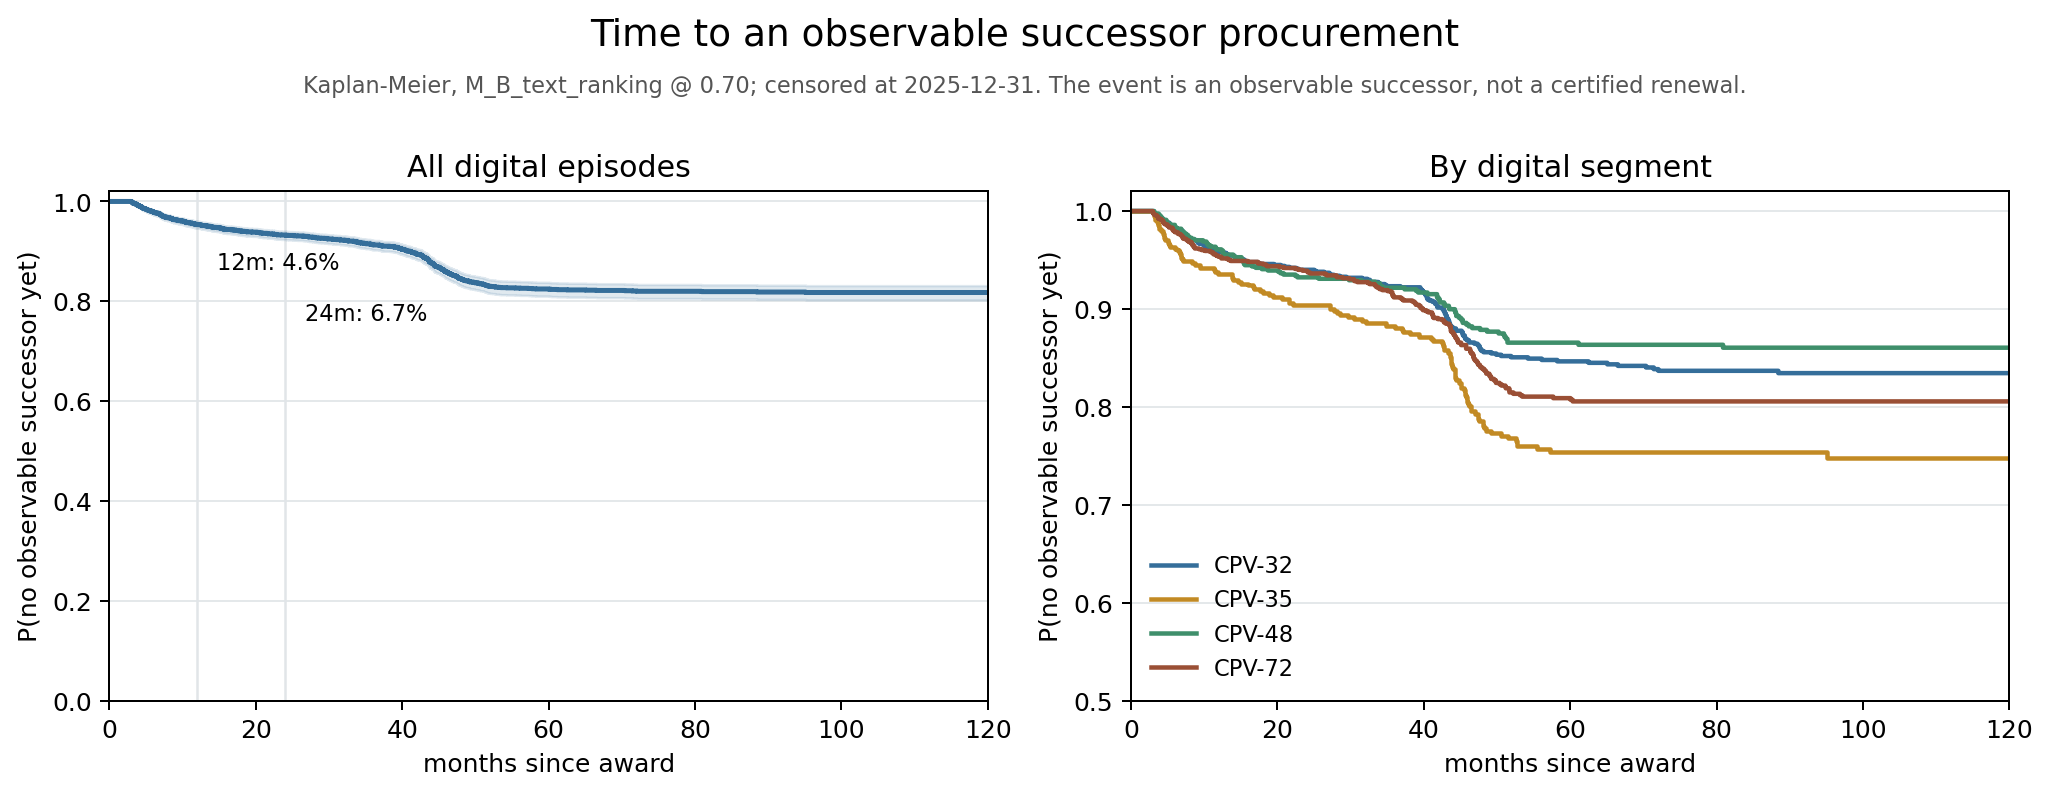
\includegraphics[width=1.0\linewidth]{figures/fig02_km_overall_and_segment.png}
\caption{Time to an observable successor procurement under the frozen \texttt{M\_B @ 0.70} rule, censored at 2025-12-31. Left: the whole cohort; the curve never falls below 0.5, so the Kaplan--Meier median is not reached, and the drop sits between 40 and 48 months. Right: by CPV division; CPV-35 separates from the other three. \textbf{The right-hand axis starts at 0.5, not 0}, so the separation appears larger than on the full scale. At-risk counts are in Annex D.}
\label{fig:km}
\end{figure}
 It is the most interesting part of the curve for Gigalis and also the most fragile: at 48 months the risk set contains only pre-2022 awards, so cohort composition changes along the curve. It should not be quoted without the at-risk counts (Annex D).

\textbf{Between-segment comparison.} The multivariate log-rank test across the four CPV segments gives a statistic of \textbf{23.45} for \(p = 3.3\times 10^{-5}\): the segments do not behave alike. Raw event rates run from 11.6 \% (CPV-48) to 20.4 \% (CPV-35).

\subsection{Conditional probabilities: the operational output}

For a procurement episode that has reached age \(a\) with no observed successor, the probability that one appears within the next \(h\) months is
\[P(T \le a+h \mid T > a) = 1 - \frac{S(a+h)}{S(a)},\]
read off the Kaplan-Meier estimator. Both 500-draw episode-bootstrap and buyer-cluster-bootstrap intervals are reported; the latter resamples buyers and preserves the dependence among their episodes.

\begingroup\footnotesize
\begin{longtable}[]{@{}
  >{\raggedleft\arraybackslash}p{(\columnwidth - 8\tabcolsep) * \real{0.2222}}
  >{\raggedleft\arraybackslash}p{(\columnwidth - 8\tabcolsep) * \real{0.2222}}
  >{\raggedright\arraybackslash}p{(\columnwidth - 8\tabcolsep) * \real{0.1667}}
  >{\raggedleft\arraybackslash}p{(\columnwidth - 8\tabcolsep) * \real{0.2222}}
  >{\raggedright\arraybackslash}p{(\columnwidth - 8\tabcolsep) * \real{0.1667}}@{}}
\toprule\noalign{}
\begin{minipage}[b]{\linewidth}\raggedleft
Episode age
\end{minipage} & \begin{minipage}[b]{\linewidth}\raggedleft
P(successor $\le$ 12 m)
\end{minipage} & \begin{minipage}[b]{\linewidth}\raggedright
95 \% CI (episode; buyer)
\end{minipage} & \begin{minipage}[b]{\linewidth}\raggedleft
P($\le$ 24 m)
\end{minipage} & \begin{minipage}[b]{\linewidth}\raggedright
95 \% CI (episode; buyer)
\end{minipage} \\
\midrule\noalign{}
\endhead
\bottomrule\noalign{}
\endlastfoot
0 months & 4.62 \% & {[}3.91; 5.24{]}; {[}3.63; 5.68{]} & 6.73 \% & {[}5.91; 7.58{]}; {[}5.25; 8.59{]} \\
12 months & 2.22 \% & {[}1.70; 2.73{]}; {[}1.38; 3.23{]} & 4.26 \% & {[}3.55; 4.98{]}; {[}3.25; 5.36{]} \\
24 months & 2.09 \% & {[}1.58; 2.60{]}; {[}1.54; 2.63{]} & 9.40 \% & {[}8.33; 10.68{]}; {[}7.69; 11.20{]} \\
\textbf{36 months} & \textbf{7.46 \%} & {[}6.52; 8.59{]}; {[}5.88; 9.06{]} & \textbf{9.69 \%} & {[}8.58; 11.12{]}; {[}7.88; 11.71{]} \\
48 months & 2.41 \% & {[}1.77; 3.07{]}; {[}1.66; 3.32{]} & 2.89 \% & {[}2.15; 3.72{]}; {[}2.08; 3.91{]} \\
\end{longtable}
\endgroup

The profile is not monotone in age: it rises into the 36-48 month shoulder and falls away after it. Buyer clustering widens several intervals but does not materially change this operational pattern. The table is therefore used as a \textbf{cohort-level watch logic}: it ranks ages and segments, it does not predict an individual episode.

\begin{figure}[htbp]
\centering
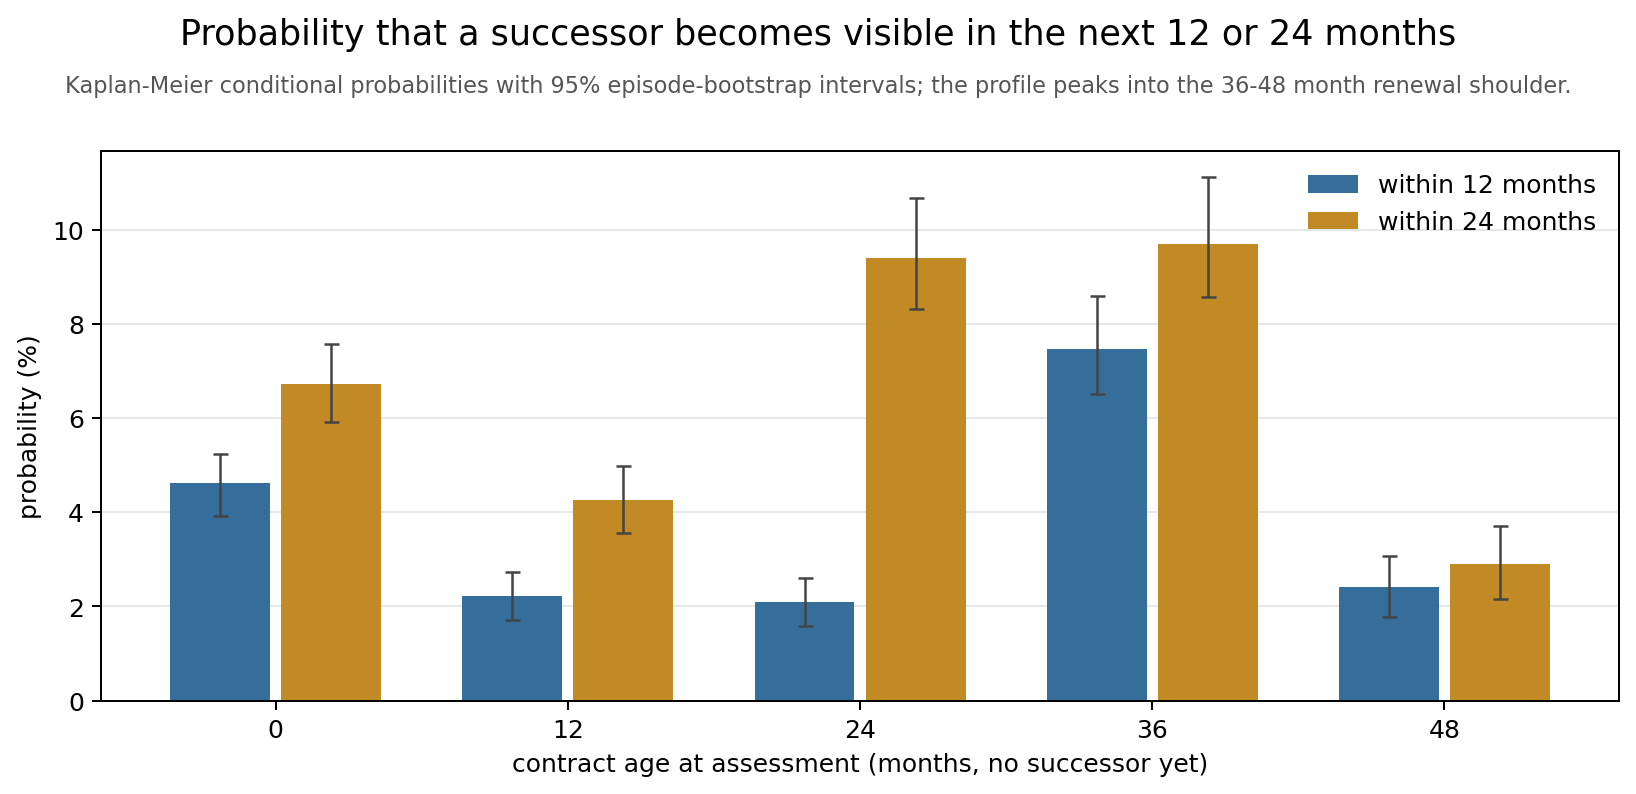
\includegraphics[width=0.85\linewidth]{figures/fig03_conditional_probabilities.png}
\caption{Probability that an observable successor appears within the next 12 or 24 months, by episode age, with 500-draw episode-bootstrap intervals. Buyer-cluster intervals are reported in the table and are somewhat wider without changing the pattern. The profile peaks around 36 months and falls away afterwards; it supports cohort-level monitoring, not individual prediction.}
\label{fig:condprob}
\end{figure}


\subsection{Cox model: comparative associations}

The proportional-hazards model \citep{cox1972},
\[h(t \mid X) = h_0(t)\exp(\beta_1X_1 + \cdots + \beta_pX_p),\]
estimates covariate effects without specifying the baseline hazard. Five covariates are retained, consistent with the one-parameter-per-ten-events rule: CPV segment, region, framework status, validated-SIREN availability, and centred award year --- eight parameters for 544 events.

\begingroup\small
\begin{longtable}[]{@{}
  >{\raggedright\arraybackslash}p{(\columnwidth - 6\tabcolsep) * \real{0.2143}}
  >{\raggedleft\arraybackslash}p{(\columnwidth - 6\tabcolsep) * \real{0.2857}}
  >{\raggedright\arraybackslash}p{(\columnwidth - 6\tabcolsep) * \real{0.2143}}
  >{\raggedleft\arraybackslash}p{(\columnwidth - 6\tabcolsep) * \real{0.2857}}@{}}
\toprule\noalign{}
\begin{minipage}[b]{\linewidth}\raggedright
Covariate
\end{minipage} & \begin{minipage}[b]{\linewidth}\raggedleft
HR
\end{minipage} & \begin{minipage}[b]{\linewidth}\raggedright
95 \% CI
\end{minipage} & \begin{minipage}[b]{\linewidth}\raggedleft
p
\end{minipage} \\
\midrule\noalign{}
\endhead
\bottomrule\noalign{}
\endlastfoot
Framework agreement & 1.751 & {[}1.435; 2.136{]} & $3.4\times 10^{-8}$ \\
\textbf{CPV-35} (ref. CPV-32) & \textbf{1.553} & {[}1.218; 1.981{]} & \textbf{$3.8\times 10^{-4}$} \\
CPV-48 & 0.828 & {[}0.638; 1.073{]} & 0.153 \\
CPV-72 & 1.056 & {[}0.850; 1.310{]} & 0.624 \\
Normandie (ref. Bretagne) & 0.800 & {[}0.640; 1.000{]} & 0.050 \\
Pays de la Loire & 1.003 & {[}0.815; 1.234{]} & 0.979 \\
Validated SIREN & 1.082 & {[}0.885; 1.323{]} & 0.443 \\
Award year (centred) & 1.107 & {[}1.066; 1.149{]} & $1.2\times 10^{-7}$ \\
\end{longtable}
\endgroup

In-sample concordance: 0.626.

This population model answers how episodes compare across the Grand Ouest cohort. In that estimand, CPV-35 episodes show earlier observable successors (HR 1.553). It is a descriptive population contrast, not an intrinsic or causal segment effect; the within-buyer sensitivity below answers a different question and attenuates this estimate.

The assumption is tested on weighted Schoenfeld residuals \citep{grambsch1994}. \textbf{The diagnostic rejects constant effects for three covariates}: award year (statistic 70.7, \(p = 4\times 10^{-17}\)), framework status (7.04, \(p = 0.008\)) and validated SIREN (6.76, \(p = 0.009\)). The award-year violation is severe and expected: award year is structurally confounded with follow-up length. These coefficients are therefore \textbf{time-averaged descriptive associations, not effects}. Stratifying on award-year bands would be cleaner; it was judged optional because the coefficients of interest barely move and nothing operational rests on this model.

\subsection{Temporal validation: a negative result}

The model is fitted once on 2015-2021 awards and scored out of time, with no refitting and no retuning.

\begingroup\footnotesize
\begin{longtable}[]{@{}
  >{\raggedright\arraybackslash}p{(\columnwidth - 12\tabcolsep) * \real{0.1111}}
  >{\raggedleft\arraybackslash}p{(\columnwidth - 12\tabcolsep) * \real{0.1481}}
  >{\raggedleft\arraybackslash}p{(\columnwidth - 12\tabcolsep) * \real{0.1481}}
  >{\raggedleft\arraybackslash}p{(\columnwidth - 12\tabcolsep) * \real{0.1481}}
  >{\raggedleft\arraybackslash}p{(\columnwidth - 12\tabcolsep) * \real{0.1481}}
  >{\raggedleft\arraybackslash}p{(\columnwidth - 12\tabcolsep) * \real{0.1481}}
  >{\raggedleft\arraybackslash}p{(\columnwidth - 12\tabcolsep) * \real{0.1481}}@{}}
\toprule\noalign{}
\begin{minipage}[b]{\linewidth}\raggedright
Window
\end{minipage} & \begin{minipage}[b]{\linewidth}\raggedleft
Train N
\end{minipage} & \begin{minipage}[b]{\linewidth}\raggedleft
Train events
\end{minipage} & \begin{minipage}[b]{\linewidth}\raggedleft
Test N
\end{minipage} & \begin{minipage}[b]{\linewidth}\raggedleft
Test events
\end{minipage} & \begin{minipage}[b]{\linewidth}\raggedleft
Train C
\end{minipage} & \begin{minipage}[b]{\linewidth}\raggedleft
\textbf{Test C}
\end{minipage} \\
\midrule\noalign{}
\endhead
\bottomrule\noalign{}
\endlastfoot
Primary, 2022-2024 & 2,470 & 392 & 1,004 & 107 & 0.606 & \textbf{0.479} \\
Sensitivity, 2022-2025 & 2,470 & 392 & 1,330 & 152 & 0.606 & \textbf{0.518} \\
\end{longtable}
\endgroup

A concordance point estimate of 0.479 is close to chance. A fixed-prediction bootstrap gives an episode-level 95\,\% interval of {[}0.415; 0.542{]} and a wider buyer-cluster interval of {[}0.360; 0.634{]}, reflecting dependence among episodes from the same buyer. The available temporal validation therefore \textbf{does not establish useful individual discrimination}; it does not mathematically rule out every moderately discriminative population value. Part of the difficulty is structural --- episodes awarded from 2022 can only contribute short gaps, and Harrell's C \citep{harrell1982} depends on the censoring distribution \citep{uno2011}, so two windows with unequal follow-up are not strictly comparable.

The result is published as it stands, and it drives a decision: \textbf{the Cox model is not used as an individual ranking engine}. The brief expected a table of the twenty contracts most likely to be renewed; producing it would convey a precision the validation does not support. The operational deliverable is therefore the conditional table of \S~5.3 and, in the annex, a \textbf{segment-stratified watch list} --- five episodes per CPV segment among those awarded since 2021 --- read off the segment-stratified Kaplan-Meier curves rather than the Cox model. The stratification is deliberate: since the conditional probability is a function of segment and age alone, a global ranking would mechanically return the highest-hazard segment at the age closest to the shoulder, implying an individual-level granularity that does not exist.

\subsection{Parametric models}

Five accelerated-failure-time families \citep{kalbfleisch2002} were fitted and compared on AIC and BIC:

\begingroup\footnotesize
\begin{longtable}[]{@{}lrrrr@{}}
\toprule\noalign{}
Model & Parameters & Log-likelihood & AIC & BIC \\
\midrule\noalign{}
\endhead
\bottomrule\noalign{}
\endlastfoot
\textbf{Generalised gamma} & 3 & $-$3,757.5 & \textbf{7,521.0} & \textbf{7,539.7} \\
Log-normal & 2 & $-$3,784.6 & 7,573.2 & 7,585.7 \\
Log-logistic & 2 & $-$3,807.3 & 7,618.6 & 7,631.1 \\
Weibull & 2 & $-$3,814.7 & 7,633.4 & 7,645.8 \\
Exponential & 1 & $-$3,829.7 & 7,661.3 & 7,667.6 \\
\end{longtable}
\endgroup

The generalised gamma wins on both criteria. It is \textbf{not} the source of the operational figures, and that choice deserves defending: every one of these families is smooth and flattens the empirical 36-48 month shoulder, which is precisely the business object; and every published horizon (12, 24 months) lies inside the observed window, where the empirical estimator needs no shape assumption. The parametric model is therefore kept as the best-fitting family and as the instrument any extrapolation beyond 31 December 2025 would use. Mechanically taking the lowest AIC to produce operational numbers would have traded a slightly better global fit for a worse rendering of the only region the user cares about.

\subsection{Robustness and sensitivity checks}

This is the most important section of the report for interpretation, because it separates what moves from what holds.

\textbf{(a) Four event definitions.}

\begingroup\footnotesize
\begin{longtable}[]{@{}
  >{\raggedright\arraybackslash}p{(\columnwidth - 10\tabcolsep) * \real{0.1304}}
  >{\raggedleft\arraybackslash}p{(\columnwidth - 10\tabcolsep) * \real{0.1739}}
  >{\raggedleft\arraybackslash}p{(\columnwidth - 10\tabcolsep) * \real{0.1739}}
  >{\raggedleft\arraybackslash}p{(\columnwidth - 10\tabcolsep) * \real{0.1739}}
  >{\raggedleft\arraybackslash}p{(\columnwidth - 10\tabcolsep) * \real{0.1739}}
  >{\raggedleft\arraybackslash}p{(\columnwidth - 10\tabcolsep) * \real{0.1739}}@{}}
\toprule\noalign{}
\begin{minipage}[b]{\linewidth}\raggedright
Arm
\end{minipage} & \begin{minipage}[b]{\linewidth}\raggedleft
Events
\end{minipage} & \begin{minipage}[b]{\linewidth}\raggedleft
Rate
\end{minipage} & \begin{minipage}[b]{\linewidth}\raggedleft
P($\le$ 12 m)
\end{minipage} & \begin{minipage}[b]{\linewidth}\raggedleft
P($\le$ 24 m)
\end{minipage} & \begin{minipage}[b]{\linewidth}\raggedleft
Median observed gap
\end{minipage} \\
\midrule\noalign{}
\endhead
\bottomrule\noalign{}
\endlastfoot
\texttt{M\_B\ @\ 0.80} strict & 296 & 7.8 \% & 2.37 \% & 3.23 \% & 35.7 months \\
\textbf{\texttt{M\_B\ @\ 0.70} primary} & \textbf{544} & \textbf{14.3 \%} & \textbf{4.62 \%} & \textbf{6.73 \%} & \textbf{31.8 months} \\
\texttt{M\_B\ @\ 0.60} loose & 853 & 22.4 \% & 8.00 \% & 11.47 \% & 26.6 months \\
\texttt{M\_C\ @\ 0.70} contrast & 1,332 & 35.1 \% & 12.21 \% & 17.98 \% & 26.1 months \\
\end{longtable}
\endgroup

A factor of 4.5 on the event count. \textbf{No absolute probability can stand alone.} Plotted together, the four survival curves shift vertically but retain a similar \textbf{shape}, with the drop between 40 and 48 months visible in all four arms. The absolute level depends strongly on the rule; the re-procurement shoulder is less sensitive to where the acceptance line is drawn.

\begin{figure}[htbp]
\centering
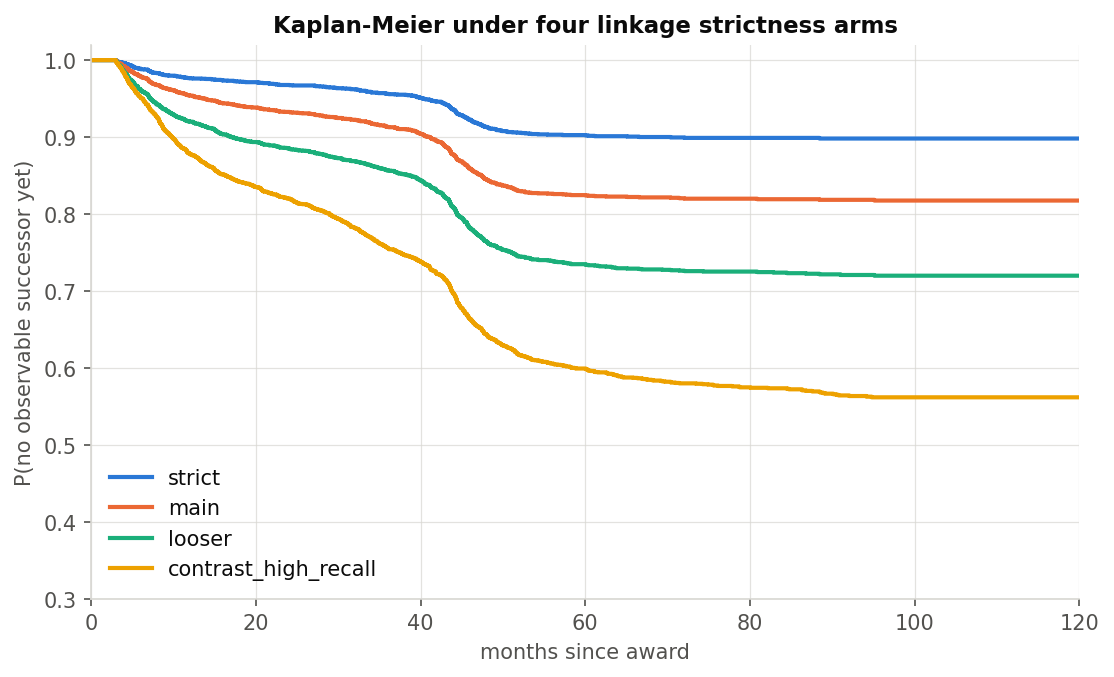
\includegraphics[width=0.85\linewidth]{figures/fig04_linkage_sensitivity.png}
\caption{Kaplan--Meier curves under the four retained linkage arms. The event count runs from 296 to 1,332 and the curves shift vertically, but they keep the same shape, including the 40--48 month shoulder. This is the report's central interpretive figure: absolute levels are conditional on the linkage rule, while the shape of the risk profile is not.}
\label{fig:sens}
\end{figure}


\textbf{(b) Borderline band.} The most fragile decisions are those whose best candidate sits near the bar. Removing the 280 episodes scoring in \([0.65; 0.75]\) --- a symmetric band fixed a priori and never searched over --- drops 133 events and gives: P($\le$ 12 m) 4.62 \% $\rightarrow$ 3.72 \%, CPV-35 HR 1.553 $\rightarrow$ \textbf{1.780}, framework HR 1.751 $\rightarrow$ 1.616. Both headline hazard ratios keep their direction.

\textbf{(c) Template-risk re-censoring.} The first two tests move the acceptance bar. But the false-positive mechanism the linkage audit identified produces links well \textbf{above} it: French award notices carry long standardised framework boilerplate on which character n-grams score highly between unrelated objects, and \texttt{M\_B} ranks candidates independently per anchor, so one episode can be accepted for several anchors. Two observable signatures define the at-risk group: word-level similarity below 0.50 (65 links), or a successor shared with another anchor (127 links) --- together \textbf{173 of the 544 links (31.8 \%)}. Those anchors are \textbf{re-censored at the cut-off} rather than deleted, because that is the counterfactual a spurious link implies: the anchor had no observed successor and should contribute its full follow-up as censored exposure. Result: P($\le$ 12 m) falls to 2.64 \%, but CPV-35 HR = \textbf{1.541} and framework HR = \textbf{1.692}. This is the test the framework finding most needed, since that boilerplate is the very text driving the mechanism.

\textbf{(d) Detectability.} The largest imbalance between linked and censored episodes is not a property of the contract at all:

\begingroup\footnotesize
\begin{longtable}[]{@{}lrrr@{}}
\toprule\noalign{}
Variable & Linked mean & Censored mean & SMD \\
\midrule\noalign{}
\endhead
\bottomrule\noalign{}
\endlastfoot
\textbf{log(candidate pool size)} & 4.787 & 3.972 & \textbf{+0.470} \\
candidate pool size & 274.3 & 188.6 & +0.285 \\
text length & 1,611 & 1,087 & +0.262 \\
framework flag & 0.265 & 0.187 & +0.187 \\
\end{longtable}
\endgroup

\texttt{M\_B} takes the maximum text score over the candidate block, and the maximum of more draws is larger: a buyer who publishes prolifically is mechanically more likely to yield an accepted link. This is an \textbf{observability} channel, not a cause of re-procurement. A sensitivity model adds \(\log(1 + \text{pool size})\):

\begingroup\footnotesize
\begin{longtable}[]{@{}lrrr@{}}
\toprule\noalign{}
Covariate & HR, main model & HR, + log(pool) & adjusted p \\
\midrule\noalign{}
\endhead
\bottomrule\noalign{}
\endlastfoot
Framework agreement & 1.751 & \textbf{1.617} & $2.6\times 10^{-6}$ \\
CPV-35 & 1.553 & \textbf{1.512} & $8.5\times 10^{-4}$ \\
log(pool size) & --- & 1.184 & $6.0\times 10^{-9}$ \\
\end{longtable}
\endgroup

Two readings follow, and they differ. \textbf{The population CPV-35 contrast is insensitive to direct pool-size adjustment}: the hazard ratio moves from 1.553 to 1.512 and remains directionally stable across event-definition checks. \textbf{The framework association is partly detectability}: roughly 14 \% of the log hazard ratio attenuates. Its direction remains positive across the main specifications, but its magnitude is smaller than the population model alone implies.

The main model is unchanged: this column is a sensitivity, not a new reference specification.

\textbf{(e) Buyer-stratified Cox.} Giving each buyer its own baseline hazard controls time-invariant buyer characteristics --- institutional procurement culture, region and persistent publication propensity among them. It does \emph{not} eliminate anchor-specific candidate-pool detectability: pool size varies within \textbf{473 of 514} buyers with multiple cohort episodes (92.0\,\%), because each anchor has a different award date and future follow-up. The pool-adjusted and buyer-stratified models therefore have distinct roles and neither replaces the other.

\begingroup\footnotesize
\begin{longtable}[]{@{}lrrr@{}}
\toprule\noalign{}
Within-buyer covariate & HR & 95\,\% CI & $p$ \\
\midrule\noalign{}
\endhead
Framework agreement & 1.497 & {[}1.150; 1.948{]} & 0.0027 \\
CPV-35 (ref. CPV-32) & 1.213 & {[}0.866; 1.699{]} & 0.262 \\
CPV-48 & 0.482 & {[}0.346; 0.672{]} & $1.7\times10^{-5}$ \\
CPV-72 & 0.831 & {[}0.627; 1.100{]} & 0.196 \\
Award year (centred) & 1.015 & {[}0.967; 1.065{]} & 0.547 \\
\bottomrule\noalign{}
\end{longtable}
\endgroup

The estimands now separate cleanly. At the Grand Ouest population level, CPV-35 episodes show earlier observable successors; within a buyer, the estimate attenuates toward 1 and is imprecise, suggesting that part of the population difference is compositional without proving confounding or refuting the population result. Framework status remains positive and statistically supported in the primary within-buyer analysis, although its magnitude attenuates; the strict event-definition arm is positive but imprecise. Buyer-stratified sensitivity also suggests slower observable-successor timing for CPV-48 within buyers. That direction is consistent across the four linkage arms, but it emerged from a sensitivity analysis and is treated as an \textbf{exploratory secondary result}, with no multiplicity-adjusted significance claim.

\subsection{What the survival analysis establishes}

Under the retained event definition, the probability that an awarded Grand Ouest digital procurement episode shows an observable successor is estimated at 4.6 \% by twelve months and 6.7 \% by twenty-four, with a marked re-procurement shoulder between 36 and 48 months. Absolute successor levels are strongly sensitive to the linkage definition, whereas several comparative patterns are more stable. At population level CPV-35 episodes show earlier successors, but the contrast attenuates within buyer; framework status remains positively associated after direct detectability and primary within-buyer controls; and the CPV-48 within-buyer slowdown is exploratory. The out-of-time point estimate is close to chance and does not establish useful individual ranking, so the Cox model is not used for that purpose.

\section{Text signal: a supervised technology taxonomy}

\subsection{Why CPV is not enough}

The cohort is defined by four CPV divisions. That is reproducible and auditable --- and coarse: CPV says a procurement is digital, not what was bought. Yet every business question Gigalis asks lives at the second level: which segments are growing, which are re-procured fastest, where to open a framework agreement. This section learns that missing variable from the text of the contract object:

\[\text{procurement object text} \longrightarrow \text{supervised classifier} \longrightarrow \text{business technology class}\]

It is an \textbf{enrichment layer}. It does not replace the CPV segmentation, which remains the cohort definition, the Cox covariate, and the axis of the time series.

\subsection{Taxonomy and corpus}

Eight substantive classes --- cloud/hosting, cybersecurity, network/telecom, IT infrastructure, business software, data/BI, AI and IT services --- plus three fallback classes that are \textbf{annotation decisions}, not missing values: \texttt{MIXED} (no dominant technology), \texttt{OTHER\_DIGITAL} (a digital purchase outside the eight), \texttt{OTHER} (a digital CPV on something that is not a technology purchase). The taxonomy was frozen before any modelling.

The corpus holds \textbf{500 manually annotated notices}, 2015-2025, all with a non-empty object text (median 14 words). Two properties constrain how it may be read. The sample is \textbf{quota-stratified}: the class proportions are a property of the annotation design, not an estimate of prevalence. And the \texttt{AI} class holds only \textbf{7 notices} across eleven years: no synthetic examples were created, no rows duplicated, no oversampling applied. The consequence is published rather than engineered away.

\subsection{Leakage prevention}

The BOAMP republishes procedures, and buyers re-run near-identical consultations a few years apart. Scoring a model on a near-copy of a document it trained on measures memorisation. Every notice is therefore assigned to a \textbf{procurement family}, defined as the union of two rules: notices already grouped into one reconstructed episode, and notices whose objects reach a character-level cosine similarity of 0.80. Each family belongs to exactly one fold.

The second rule is not redundant: the first alone gives 486 groups; adding the second merges 39 near-duplicate pairs, of which \textbf{29 sit in different episodes} and would otherwise have been split across folds. The result is \textbf{459 families}, none spanning two folds.

One side effect deserves mention: \textbf{3 families contain notices with near-identical text but different labels} --- videoconference services labelled \texttt{NETWORK\_TELECOM} in 2017 and \texttt{OTHER\_DIGITAL} in 2021; an infrastructure-as-a-service procurement labelled \texttt{MIXED} in 2017 and \texttt{CLOUD\_HOSTING} in 2021. No label was changed: no evidence decides which reading is right, and editing labels after seeing the model's errors is how a corpus is fitted to its classifier. They are recorded as an empirical floor on attainable accuracy.

\subsection{Representation and models}

The input is the \texttt{objet} field alone. Normalisation is deliberately light --- mojibake repair, NFC, lowercasing, whitespace --- and \textbf{accents are preserved}, with no stemming: the classes are distinguished by words such as \emph{cybersécurité}, \emph{logiciel métier} and \emph{intelligence artificielle}, and flattening French orthography would discard the evidence. Features are TF-IDF word n-grams \citep{salton1988}; both unigrams and unigrams-plus-bigrams were in the search space, and \textbf{every fold selected unigrams alone}, the bigram vocabulary being too sparse across 500 short documents.

Excluded from the features by design: buyer identity, geography, dates, amounts, procedure type, framework status, notice identifiers, every linkage variable, and CPV --- which serves as the comparator.

Six specifications were compared on identical folds, with hyperparameters selected by inner cross-validation \emph{inside each training fold}:

\begingroup\footnotesize
\begin{longtable}[]{@{}llr@{}}
\toprule\noalign{}
Model & Features & Out-of-fold macro-F1 \\
\midrule\noalign{}
\endhead
\bottomrule\noalign{}
\endlastfoot
Majority class & --- & 0.027 \\
CPV only & CPV codes & 0.441 \\
CPV + BOAMP descriptors & administrative & 0.473 \\
TF-IDF + logistic regression & text & 0.670 \\
\textbf{TF-IDF + class-weighted logistic regression} & text & \textbf{0.744} \\
TF-IDF + linear SVM & text & 0.718 \\
TF-IDF + class-weighted linear SVM & text & 0.715 \\
\end{longtable}
\endgroup

\subsection{The headline result}

\begingroup\small
\begin{longtable}[]{@{}
  >{\raggedright\arraybackslash}p{(\columnwidth - 4\tabcolsep) * \real{0.3000}}
  >{\raggedleft\arraybackslash}p{(\columnwidth - 4\tabcolsep) * \real{0.4000}}
  >{\raggedright\arraybackslash}p{(\columnwidth - 4\tabcolsep) * \real{0.3000}}@{}}
\toprule\noalign{}
\begin{minipage}[b]{\linewidth}\raggedright
Comparison
\end{minipage} & \begin{minipage}[b]{\linewidth}\raggedleft
Macro-F1
\end{minipage} & \begin{minipage}[b]{\linewidth}\raggedright
95 \% CI (family bootstrap)
\end{minipage} \\
\midrule\noalign{}
\endhead
\bottomrule\noalign{}
\endlastfoot
TF-IDF + class-weighted logistic regression & \textbf{0.7442} & {[}0.682; 0.791{]} \\
Best CPV / descriptor comparator & 0.4731 & {[}0.413; 0.526{]} \\
\textbf{Paired difference} & \textbf{+0.2711} & \textbf{{[}0.201; 0.340{]}} \\
\end{longtable}
\endgroup

The interval on the difference excludes zero. Three precautions make this result solid rather than trivial: both sides use \textbf{the same folds} and \textbf{the same hyperparameter search budget}; the difference is \textbf{paired} fold by fold; and the bootstrap resamples \textbf{procurement families}, the unit at which dependence exists, rather than notices.

In other words, the text of the notices carries business information the administrative vocabulary does not. The crosswalk makes this concrete:

\begingroup\footnotesize
\begin{longtable}[]{@{}
  >{\raggedright\arraybackslash}p{(\columnwidth - 8\tabcolsep) * \real{0.1765}}
  >{\raggedright\arraybackslash}p{(\columnwidth - 8\tabcolsep) * \real{0.1765}}
  >{\raggedleft\arraybackslash}p{(\columnwidth - 8\tabcolsep) * \real{0.2353}}
  >{\raggedleft\arraybackslash}p{(\columnwidth - 8\tabcolsep) * \real{0.2353}}
  >{\raggedright\arraybackslash}p{(\columnwidth - 8\tabcolsep) * \real{0.1765}}@{}}
\toprule\noalign{}
\begin{minipage}[b]{\linewidth}\raggedright
CPV division
\end{minipage} & \begin{minipage}[b]{\linewidth}\raggedright
Dominant class
\end{minipage} & \begin{minipage}[b]{\linewidth}\raggedleft
Dominant count
\end{minipage} & \begin{minipage}[b]{\linewidth}\raggedleft
Purity
\end{minipage} & \begin{minipage}[b]{\linewidth}\raggedright
Other classes $\ge$ 100 episodes
\end{minipage} \\
\midrule\noalign{}
\endhead
\bottomrule\noalign{}
\endlastfoot
CPV-32 (telecoms) & Network/telecom & 426 / 1,152 & 0.370 & Other digital 202; business software 146; IT infrastructure 128 \\
CPV-35 (security) & Network/telecom & 165 / 564 & 0.293 & Other 114; cybersecurity 106 \\
CPV-48 (software) & Business software & 348 / 790 & 0.441 & --- \\
CPV-72 (IT services) & IT services & 325 / 1,294 & 0.251 & Business software 310; network/telecom 204; other digital 165 \\
\end{longtable}
\endgroup

Two readings. The mean purity of a CPV segment against the learnt taxonomy is \textbf{0.34}: no division corresponds to a technology. And the largest division, CPV-72, is the least pure of the four (0.251): what the administrative vocabulary calls ``IT services'' in fact spans four business families of comparable size. One telling detail: CPV-32 and CPV-35, two distinct divisions of the vocabulary, share the \textbf{same} dominant predicted class.

\subsection{What the classifier can and cannot do}

\begingroup\footnotesize
\begin{longtable}[]{@{}lrrrr@{}}
\toprule\noalign{}
Class & Precision & Recall & F1 & Support \\
\midrule\noalign{}
\endhead
\bottomrule\noalign{}
\endlastfoot
DATA\_BI & 0.923 & 0.828 & \textbf{0.873} & 29 \\
OTHER & 0.923 & 0.800 & 0.857 & 15 \\
BUSINESS\_SOFTWARE & 0.798 & 0.898 & 0.845 & 88 \\
NETWORK\_TELECOM & 0.810 & 0.840 & 0.824 & 81 \\
CYBERSECURITY & 0.848 & 0.722 & 0.780 & 54 \\
IT\_SERVICES & 0.778 & 0.757 & 0.767 & 74 \\
IT\_INFRASTRUCTURE & 0.702 & 0.717 & 0.710 & 46 \\
OTHER\_DIGITAL & 0.655 & 0.679 & 0.667 & 53 \\
AI & 0.800 & 0.571 & \emph{0.667} & \textbf{7} \\
CLOUD\_HOSTING & 0.731 & 0.594 & 0.655 & 32 \\
MIXED & 0.482 & 0.619 & 0.542 & 21 \\
\end{longtable}
\endgroup

Macro-F1 0.741 (fold standard deviation 0.034), weighted F1 0.765, accuracy 0.766. Two aggregations coexist and should be kept apart: 0.741 is the \textbf{mean across the three folds}, whereas the headline figure of \S~6.5, 0.744, is computed \textbf{out of fold on the pooled 500 predictions}. The gap is the expected one between an average of per-fold scores and a single score over all predictions.

Three readings. The reliable classes are \texttt{CYBERSECURITY}, \texttt{NETWORK\_TELECOM}, \texttt{BUSINESS\_SOFTWARE}, \texttt{DATA\_BI}, \texttt{IT\_SERVICES} and \texttt{OTHER}. \texttt{MIXED} is weak, which is consistent with its definition as the bucket for procurements without a dominant technology. And \textbf{\texttt{AI} is not interpretable}: its F1 of 0.667 rests on three correct predictions; a high number would be a small-sample artefact and a low one equally uninformative.

Error analysis on thirty representative cases gives: 16 model errors, 7 taxonomy-boundary ambiguities, 4 genuinely multi-technology procurements, 2 annotation inconsistencies, 1 object text too poor to decide. Close to half the errors therefore come from class definitions or from missing information rather than from model capacity.

\textbf{Temporal robustness.} Training 2015-2022 (n = 393), test 2023-2025 (n = 107), with the 4 boundary-straddling families assigned to training --- which costs test observations and cannot flatter the result. All-class macro-F1 0.662, but \textbf{0.815 on classes with test support of at least 10}. The vocabulary of recent notices has not drifted for the high-volume classes; nothing can be concluded for the six classes with thin recent support.

\subsection{Two negative decisions, taken against pre-written criteria}

\textbf{The transformer was considered but not evaluated.} The internship brief proposed evaluating a transformer and allowed a classical model to remain if any incremental gain were small; it did not itself instruct the project to skip CamemBERT \citep{martin2020}. The project later adopted a pre-specified complexity-escalation rule: escalate only if the classical model were materially inadequate (macro-F1 \textless{} 0.55) and fewer than half its errors arose from label ambiguity or missing information. The classical model reaches 0.741, training F1 is near saturation, validation F1 rises from 0.434 to 0.747 as labelled support grows, and error analysis points substantially to taxonomy and annotation ambiguity. The escalation criterion was therefore not met. The indicated next improvement is additional high-quality annotation, ideally with a second independent annotator and targeted rare-class coverage, not a wider post-hoc hyperparameter search or transformer run.

\textbf{Calibration was evaluated and rejected.} The published confidence is the raw predicted probability of the logistic regression. Platt scaling was estimated inside the same grouped splits and judged against a pre-specified rule: adopt it only if it cuts expected calibration error by at least 0.02 \textbf{and} costs at most 0.02 macro-F1. It cut the error by 0.1405 --- condition met --- but cost 0.0364 macro-F1, exceeding the budget. The rule was not relaxed to admit it.

The deployed score is therefore an \textbf{uncalibrated confidence score}. Its out-of-fold reliability is measured: observed accuracy rises from 0.52 in the {[}0, 0.3) bin to 1.00 in the {[}0.9, 1.0) bin, but the gap between stated confidence and observed accuracy is positive in every bin above 0.3 --- the score \textbf{understates} its own hit rate, with an expected calibration error of 0.350. It is therefore usable as a \textbf{ranking and a filter} --- at the 0.70 operational cutoff, out-of-fold accuracy is 0.956 on the 9 \% of notices that clear it, against 0.750 below --- but a confidence value is not the probability that the label is correct. Two reasons: the miscalibration above, and the fact that the corpus is quota-stratified while the deployment population is not, so the class prior the classifier encodes is an artefact of the annotation design.

\subsection{Deployment}

The model is refitted on all 500 labels and applied to the \textbf{3,800 cohort episodes} through the object text of each episode's origin notice. That refit has no validation score and none is reported: the evidence for the model is the grouped cross-validation and the temporal check above. Every episode receives exactly one predicted class and one confidence value; none is discarded. \textbf{235 episodes (6.2 \%)} clear the 0.70 cutoff.

Predicted composition: \texttt{NETWORK\_TELECOM} 859, \texttt{BUSINESS\_SOFTWARE} 854, \texttt{IT\_SERVICES} 492, \texttt{OTHER\_DIGITAL} 462, \texttt{CYBERSECURITY} 316, \texttt{IT\_INFRASTRUCTURE} 298, \texttt{OTHER} 173, \texttt{MIXED} 139, \texttt{CLOUD\_HOSTING} 115, \texttt{DATA\_BI} 86, \texttt{AI} 6. \textbf{These counts are not market shares}: they are predictions carrying the error rate of \S~6.6, over a cohort defined by an inclusive CPV rule.

\begin{figure}[htbp]
\centering
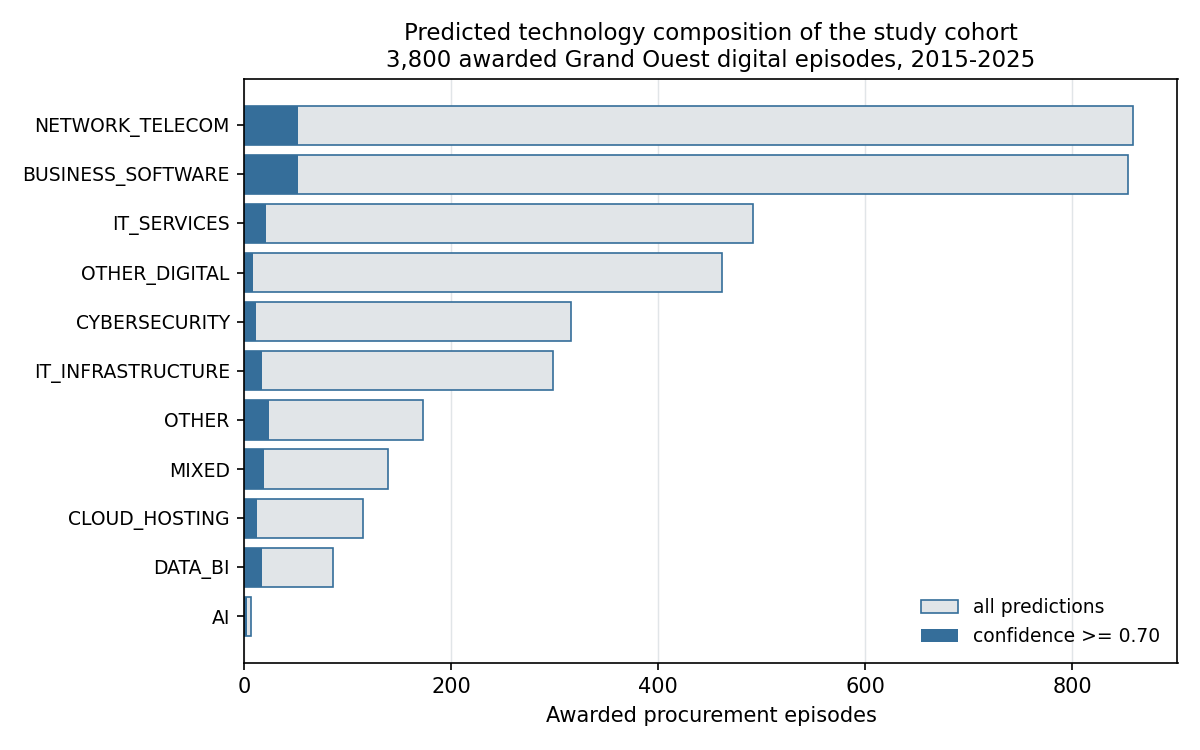
\includegraphics[width=0.85\linewidth]{figures/fig06_technology_composition.png}
\caption{Predicted technology composition of the 3,800 cohort episodes, with the share clearing the 0.70 confidence cutoff overlaid. \texttt{NETWORK\_TELECOM} and \texttt{BUSINESS\_SOFTWARE} dominate at almost identical size, while \texttt{AI} holds six episodes across eleven years. The dark portion is small everywhere, a reminder that the deployed confidence score is conservative. \textbf{These counts are predictions, not market shares.}}
\label{fig:techcomp}
\end{figure}

\section{Downstream use of the predictions}

\subsection{Two gates before any use}

Nothing was re-run mechanically for eleven classes. A class enters downstream analysis only by clearing \textbf{both} gates, fixed before any curve was fitted.

\textbf{Gate A --- classifier evidence.} Does the label mean anything? A class the model cannot separate produces a group that mixes several technologies, and a curve fitted to it estimates the mixture. The gate requires a substantive class, annotated support of at least 10, and out-of-fold F1 of at least 0.65. The three fallback classes are excluded outright: \texttt{OTHER\_DIGITAL} simultaneously holds video surveillance, RFID and website maintenance; placing that bucket beside cybersecurity in a ``comparison across technologies'' would invite reading the heterogeneity of the bucket as a technology effect.

\textbf{Gate B --- statistical support.} At least 100 episodes and 20 events. A perfectly classified class with fourteen episodes and one event cannot carry a curve.

Five classes of eleven clear both: \texttt{CYBERSECURITY}, \texttt{NETWORK\_TELECOM}, \texttt{IT\_INFRASTRUCTURE}, \texttt{BUSINESS\_SOFTWARE}, \texttt{IT\_SERVICES}. \texttt{CLOUD\_HOSTING} (115 episodes, 11 events) and \texttt{DATA\_BI} (86, 15) fail Gate B; \texttt{AI} fails both.

\textbf{What Gate A costs.} The same log-rank test over every class clearing the statistical gate alone --- that is, with the residual classes reinstated --- gives \(p = 0.000119\) against \(p = 0.0363\) with the gate. The gate \textbf{weakens} the result, and it was kept. That is published in the technical report, and it is the strongest available evidence that the analysis was not steered toward a result.

\subsection{Survival by technology}

\begingroup\footnotesize
\begin{longtable}[]{@{}lrrrr@{}}
\toprule\noalign{}
Class & Episodes & Events & P(successor $\le$ 24 m) & At risk at 24 m \\
\midrule\noalign{}
\endhead
\bottomrule\noalign{}
\endlastfoot
BUSINESS\_SOFTWARE & 854 & 106 & 8.57 \% & 673 \\
NETWORK\_TELECOM & 859 & 140 & 6.49 \% & 716 \\
CYBERSECURITY & 316 & 60 & 6.46 \% & 246 \\
IT\_SERVICES & 492 & 72 & 6.17 \% & 393 \\
IT\_INFRASTRUCTURE & 298 & 38 & 6.11 \% & 239 \\
\end{longtable}
\endgroup

The multivariate log-rank test over these five classes gives a statistic of 10.26 for \(p = 0.0363\) on 416 events: \textbf{the five sufficiently supported predicted technology groups show evidence of different observable-successor timing}. The spread between extremes is 2.5 points at 24 months.

Confidence in this secondary descriptive result is moderate, for three cumulative reasons: the event is an accepted observable successor under the retained rule, not a renewal; the class labels are \textbf{predictions} carrying the error rate of \S~6.6, which does not propagate into the published intervals; and the comparison is unadjusted for buyer and procedure differences. It does not support a causal technology effect.

\subsection{Trends by technology}

Five quarterly series use the same 2015Q2--2025Q4 observation window as the CPV series, with recent slopes fitted over the last twelve quarters. \textbf{None shows a recent linear trend}, before or after multiplicity correction. The smallest raw p-value is 0.194 (\texttt{IT\_SERVICES}, slope $+0.45$ episodes per quarter; Holm 0.972); the strongest negative slope is \texttt{BUSINESS\_SOFTWARE} at $-0.76$ (raw $p=0.248$; Holm 0.992). The reading is therefore: at this noise level, \textbf{no recent technology trend is established}.

\subsection{The three inherited uncertainties}

Every technology-level figure inherits, in this order: \textbf{linkage uncertainty} (the event itself depends on the rule, \S~5.7), \textbf{classifier uncertainty} (macro-F1 0.744, with errors concentrated on definitional boundaries), and \textbf{sampling uncertainty} (the published intervals). Only the third appears in the confidence intervals. That is acceptable for a layer explicitly presented as enrichment; it would not be for a reference analysis.

\section{Trends and change-point detection}

\subsection{Constructing the series}

For a segment \(s\) and quarter \(q\), the count is
\[N_{s,q} = \sum_i \mathbf{1}(S_i = s,\ Q_i = q).\]
The series span \textbf{43 quarters} (2015Q2 to 2025Q4); the partial first quarter of 2015 is excluded and every subsequent quarter is represented, zeros included. Amount series are absent, for want of a validated canonical awarded value (\S~3.4).

The objective, as the brief states, is not to forecast: it is to \textbf{date and qualify changes}.

\subsection{Three instruments, three different questions}

\textbf{PELT} \citep{killick2012} minimises
\[\sum_{r=0}^{m}\mathcal{C}\big(y_{\tau_r+1:\tau_{r+1}}\big) + \beta m,\]
where \(\mathcal{C}\) is within-segment squared error and \(\beta = \lambda\log(n)\) after standardisation. The first term rewards fit; the second charges a fixed price per break, which is what stops the optimum from placing a break between every pair of quarters. The central result uses \(\lambda = 1\), with sensitivity at 0.5 and 2.0, and \textbf{a break is declared stable only if it appears within one quarter under all three penalties}. That requirement eliminates half the candidate breaks.

\textbf{ADF and KPSS} test opposite null hypotheses --- unit root for the first, level stationarity for the second --- and are therefore read together \citep{dickey1979,kwiatkowski1992}. They are not forced to agree: disagreement means the series is not cleanly classified over so short a window, and that is the useful information.

\textbf{The hidden Markov model} with three states is fitted on the \textbf{quarter-over-quarter change} \(\Delta N_t\), not on the level. Its states therefore describe a typical direction of change --- decline, plateau, growth --- not a segment's activity level. The reported figure is a posterior probability of the current state, not a forecast; the general framework is Markov regime switching \citep{hamilton1989}.

\subsection{Signal matrix}

\begingroup\footnotesize
\begin{longtable}[]{@{}
  >{\raggedright\arraybackslash}p{(\columnwidth - 14\tabcolsep) * \real{0.1071}}
  >{\raggedright\arraybackslash}p{(\columnwidth - 14\tabcolsep) * \real{0.1071}}
  >{\raggedleft\arraybackslash}p{(\columnwidth - 14\tabcolsep) * \real{0.1429}}
  >{\raggedleft\arraybackslash}p{(\columnwidth - 14\tabcolsep) * \real{0.1429}}
  >{\raggedleft\arraybackslash}p{(\columnwidth - 14\tabcolsep) * \real{0.1429}}
  >{\raggedleft\arraybackslash}p{(\columnwidth - 14\tabcolsep) * \real{0.1429}}
  >{\raggedright\arraybackslash}p{(\columnwidth - 14\tabcolsep) * \real{0.1071}}
  >{\raggedright\arraybackslash}p{(\columnwidth - 14\tabcolsep) * \real{0.1071}}@{}}
\toprule\noalign{}
\begin{minipage}[b]{\linewidth}\raggedright
Segment
\end{minipage} & \begin{minipage}[b]{\linewidth}\raggedright
Recent direction
\end{minipage} & \begin{minipage}[b]{\linewidth}\raggedleft
Slope\\(ep./qtr)
\end{minipage} & \begin{minipage}[b]{\linewidth}\raggedleft
Raw p
\end{minipage} & \begin{minipage}[b]{\linewidth}\raggedleft
Holm p
\end{minipage} & \begin{minipage}[b]{\linewidth}\raggedleft
BH p
\end{minipage} & \begin{minipage}[b]{\linewidth}\raggedright
Reading
\end{minipage} & \begin{minipage}[b]{\linewidth}\raggedright
Last stable break
\end{minipage} \\
\midrule\noalign{}
\endhead
\bottomrule\noalign{}
\endlastfoot
Overall & stable or uncertain & $-$0.11 & 0.921 & 1.000 & 0.989 & no signal & --- \\
CPV-32 & stable or uncertain & $-$0.01 & 0.989 & 1.000 & 0.989 & no signal & 2020Q2 \\
CPV-35 & stable or uncertain & +0.03 & 0.923 & 1.000 & 0.989 & no signal & --- \\
\textbf{CPV-48} & \textbf{decline} & \textbf{$-$0.84} & \textbf{0.032} & 0.159 & 0.159 & \textbf{nominal signal only} & 2024Q1 \\
CPV-72 & stable or uncertain & +0.70 & 0.285 & 1.000 & 0.714 & no signal & 2021Q1 \\
\end{longtable}
\endgroup

Five slopes are fitted and read at once, so the raw p-values are reported beside Holm \citep{holm1979} and Benjamini--Hochberg \citep{benjamini1995} adjustments. A segment whose raw p clears the pre-declared exploratory level of 0.10 but whose Holm p does not is \textbf{a nominal signal to monitor, not a finding}.

That is the case of CPV-48, and it is the one row in the table requiring an editorial decision. It is presented as it stands: the recent decline in CPV-48 procurement is the clearest signal in the panel, it does not survive correction for the five segments tested, and it justifies watching for a few more quarters --- not a conclusion, still less a forecast.

\subsection{Breaks and regimes}

Only three breaks are stable under all three penalties: CPV-32 in 2020Q2, CPV-48 in 2024Q1 and CPV-72 in 2021Q1. Neither the overall series nor CPV-35 carries one: their candidate breaks disappear as soon as the penalty changes. \textbf{None is attributed to a cause.} A PELT break dates a change in level; it does not say why. Attributing the 2020Q2 break to the pandemic would be plausible and undemonstrated, and the report abstains: such attributions require documentary evidence and stakeholder validation.

The hidden Markov model places the overall series, CPV-32 and CPV-72 in a growth regime in the final quarter (posterior probabilities 0.750, 0.992 and 0.594). That label may look inconsistent with the null twelve-quarter slopes; it is not. The slope summarises twelve quarters, the regime describes the most recent change. The two are complementary, and the report does not reconcile them artificially.

\subsection{What the trend analysis establishes}

Over the observed window, \textbf{no CPV segment shows a recent linear trend surviving multiplicity correction}, and neither does any technology series. Three level shifts are stably dated. The operational reading is therefore a monitoring arrangement: keep watching all segments, and follow CPV-48 as a lead to investigate. This is a weaker result than the brief hoped for: forty-three quarters, often with low counts, leave limited power for recent-trend inference.

\section{Discussion}

\subsection{A. What the work establishes with reasonable confidence}

\textbf{The text of the notices carries a business segmentation that CPV does not.} This is the best-established result of the internship: a paired difference of +0.271 macro-F1, interval {[}0.201; 0.340{]}, estimated at the correct level of aggregation, on identical folds with an identical search budget. It answers the brief's text-signal problem directly, and it has an immediate practical consequence: a technology-level reading is possible where the administrative vocabulary does not allow one.

\textbf{The pipeline is reproducible and structurally coherent.} Every integrity check passes, each stage replays from a single command, and a cross-artifact validator checks that the published documents and the configurations say the same thing.

\textbf{No multiplicity-robust recent linear trend is established.} This holds for the CPV and predicted-technology panels after using the same 2015Q2--2025Q4 observation window. The CPV-48 raw signal remains exploratory.

\textbf{Useful individual Cox ranking is not demonstrated.} The out-of-time point estimate is 0.479 and the conservative buyer-cluster interval is wide; that evidence supports the operational decision not to rank individual episodes.

\subsection{B. What the models indicate, conditionally}

\textbf{The probability levels.} 4.6 \% at twelve months and 6.7 \% at twenty-four, with a re-procurement shoulder at 36-48 months, \textbf{under the retained event definition}. These figures vary by a factor of four and a half with the linkage rule; they must never be quoted alone. Buyer-cluster intervals are somewhat wider but preserve the age profile.

\textbf{Population CPV comparisons.} CPV-35 episodes show earlier observable successors across the Grand Ouest population (HR 1.553), and the direction is stable to event-definition and direct pool-size perturbations. The estimate attenuates to 1.213 within buyer, so the population contrast is partly compositional and is not an intrinsic segment effect. The slower within-buyer CPV-48 pattern is exploratory.

\textbf{The framework association.} Framework episodes show a successor earlier (HR 1.751). It falls to 1.617 under direct pool-size adjustment and 1.497 in the primary within-buyer analysis. The association remains positive across main specifications and statistically supported in the primary within-buyer model, while the strict arm is imprecise: directional stability is not significance in every test.

\textbf{Predicted technologies show evidence of different timing} (\(p = 0.036\) over five classes and 416 events). This is secondary and descriptive: labels are predicted, events are constructed, and the comparison is unadjusted for buyer and procedure differences.

\subsection{C. What remains uncertain}

In order of importance: \textbf{linkage precision} is not independently validated (0.875 on eight links, CI {[}0.529; 0.978{]}; 0.700 in the model-assisted review, below the 0.80 target); the reference is \textbf{internal validation}, since operating-point and candidate-generation decisions used its evidence; \textbf{absolute levels} depend on the rule; the Cox model has \textbf{no demonstrated useful out-of-time discrimination}; the annotation corpus has \textbf{no inter-annotator agreement}; and the reference's \textbf{recall} is not independent of the score it evaluates.

\subsection{D. What Gigalis can use now}

Three uses are supported by the available evidence.

\textbf{Cohort-level monitoring, not contract-level.} The conditional probability table by age and segment (\S~5.3) identifies which \emph{groups} of episodes are entering the window where a successor becomes more visible. The 36-48 month shoulder is the main monitoring window. CPV-35 is elevated at population level, with the within-buyer qualification stated above. This is a rule for prioritising human attention, not an individual score.

\textbf{A usable business segmentation.} The eight technology classes give a reading of the regional portfolio that the four CPV divisions do not --- with a mean CPV-segment purity of 0.34, each division mixes several business families. Used at aggregate level, with the confidence filter for demanding uses, it can map activity by technology.

\textbf{A reproducible measurement instrument.} The pipeline can be re-run each quarter on updated data. That may be the most durable contribution: Gigalis holds a documented instrument whose limits are known, rather than a number.

\subsection{E. What should not be operationalised}

A \textbf{per-contract renewal score}, in any form: the out-of-time validation forbids it. An \textbf{individual ranking of contracts to watch} derived from the Cox model, for the same reason. Reading a \textbf{predicted technology class as an observed attribute} of a procurement, or its counts as market shares. A \textbf{trend forecast} by segment. And any \textbf{external communication} quoting the linkage precision as validated performance.

\subsection{F. What would add the most next}

\begin{enumerate}
\def\labelenumi{\arabic{enumi}.}
\tightlist
\item
  \textbf{An independent human review} of a blinded, re-drawn and pre-specified sample of accepted links. It is the only gate before any precision claim, and it is worth more than a fifth linkage method.
\item
  \textbf{A second technology annotation pass} by a different annotator, enabling a Cohen's $\kappa$. The learning curve is still rising at n = 500: more annotation beats a more complex model.
\item
  \textbf{Gigalis membership data} (member identity, adoption dates), without which the brief's causal question --- does opening a pooled framework agreement change members' purchasing behaviour? --- remains a staggered-adoption difference-in-differences design \citep{callaway2021}, described but not estimated.
\item
  \textbf{A separate experiment on individual prediction}, if that line is prioritised: award-time variables only (object text, buyer history), a temporal validation declared in advance, a success criterion announced beforehand, and publication of the result even if negative. The trap is named: candidate-pool size would raise concordance by learning to predict \emph{who is detectable}, not \emph{who renews}.
\end{enumerate}

\section{Limitations}

Ranked by what they can do to the results, not by category.

\textbf{1. Linkage validation is not independent.} \emph{Mechanism}: the reference labels come from a language-model pass spot-checked by sampling, the 60-pair review is likewise model-assisted, and project history shows that operating-point and candidate-generation decisions used reference evidence including the designated locked stratum. \emph{Effect}: the reported metrics are internal validation rather than a fully untouched test; any precision figure is provisional, and the conservative review gives 0.700, below target. \emph{Mitigation in place}: strict exact-successor accounting, intervals published everywhere, frozen post-development policy, and an independent review protocol with its sample prepared.

\textbf{2. Linkage errors distort both status and timing.} \emph{Mechanism}: a false link creates an event and its date; a missed link creates censoring. \emph{Effect}: absolute levels are not a lower bound, contrary to what a quick reading would suggest. \emph{Mitigation}: four event arms, the borderline band, template-risk re-censoring, and an editorial rule --- never quote a level without its range.

\textbf{3. Detectability and buyer dependence.} \emph{Mechanism}: the score is a maximum over a block, blocks vary greatly in size, and several episodes belong to one buyer. Candidate-pool size varies within 92\,\% of multi-episode buyers, so buyer stratification does not eliminate this anchor-level channel. \emph{Effect}: prolific buyers produce more observable links and episode-level intervals can be too narrow. \emph{Mitigation}: direct pool-size adjustment, a distinct within-buyer Cox sensitivity, and buyer-cluster bootstrap intervals for the operational KM quantities.

\textbf{4. Technology labels are predictions.} \emph{Mechanism}: macro-F1 of 0.744, with errors concentrated on definitional boundaries. \emph{Effect}: every technology-level figure carries a measurement error that does not enter its intervals. \emph{Mitigation}: two gates before any downstream use, an editorial rule forbidding treatment of a predicted class as an observed attribute, and exclusion of the fallback classes.

\textbf{5. The annotation corpus has no reliability measure.} \emph{Mechanism}: a single pass, no annotator identifier, no second independent reading. \emph{Effect}: taxonomy reproducibility, ambiguity and label reliability cannot be quantified. \emph{Mitigation}: three internal inconsistencies documented, annotation quotas flagged, \texttt{AI} declared unevaluable. Future work should independently annotate a pre-specified subset, compute Cohen's $\kappa$ or another suitable agreement statistic, and review disagreement patterns. Agreement would diagnose label reliability; it would not mathematically define a maximum achievable macro-F1.

\textbf{6. The Cox model violates proportional hazards.} \emph{Mechanism}: three covariates, award year severely so, structurally confounded with follow-up length. \emph{Effect}: the coefficients are descriptive time averages. \emph{Mitigation}: diagnostic published, interpretation restricted, no predictive use.

\textbf{7. The cohort is broader than its name.} \emph{Mechanism}: an any-CPV-code rule at episode level. \emph{Effect}: 30.9 \% of episodes have a main CPV outside the perimeter. \emph{Mitigation}: explicit phrasing, and measurement of the segment tie-break effect (94.7 \% agreement).

\textbf{8. The time series are short and noisy.} \emph{Mechanism}: 43 quarters, low counts, a documented completeness break in 2025. \emph{Effect}: no trend survives correction; change-point detection proposes candidates without explaining them. \emph{Mitigation}: break stability required under three penalties, multiplicity correction in both test families, and an explicit refusal to forecast.

\textbf{9. Geographic and temporal reach.} The results concern the Grand Ouest, 2015-2025, for contracts published in the BOAMP. They do not extend to France as a whole, to below-threshold purchases, or to procurements routed through a central purchasing body without their own publication.

\section{Conclusion}

The internship was meant to estimate the probability that a digital procurement generates an identifiable purchasing need within twelve to twenty-four months. It produced something else, and that difference is the main result.

\textbf{What was built.} A reproducible chain from 1,620,712 official BOAMP notices to a cohort of 3,800 reconstructed awarded Grand Ouest procurement episodes containing a digital CPV code, with an observable-successor variable whose quality is measured rather than assumed and a cross-artifact validator that checks the published documents and code agree.

\textbf{What was learnt about timing.} Under the retained event definition, the probability that an episode shows an observable successor is estimated at 4.6 \% within twelve months and 6.7 \% within twenty-four, with a re-procurement shoulder between 36 and 48 months. At population level CPV-35 episodes show earlier successors, but the contrast attenuates within buyer. Framework status remains positively associated after direct detectability and primary within-buyer controls, with a smaller magnitude.

\textbf{What survived the robustness tests.} Absolute successor levels are strongly sensitive to the linkage definition, whereas several comparative patterns are more stable. Robustness to event definition is distinct from robustness to buyer composition: CPV-35 is stable across event-definition perturbations but attenuates within buyer; framework remains positive but smaller; CPV-48 emerges principally in the within-buyer sensitivity and remains exploratory.

\textbf{What the text workstream added.} A supervised classifier on the contract object alone separates eleven business technology classes at an out-of-fold macro-F1 of 0.744, against 0.473 for the best CPV-based comparator on identical folds and budget: a paired difference of +0.271 whose interval excludes zero. Text therefore carries business information the administrative vocabulary does not. Its predictions, filtered through two explicit gates, reveal a difference in timing across technologies (\(p = 0.036\)).

\textbf{What the trend analysis showed.} Little, and that is a result: no segment slope survives correction for multiple testing. Three level shifts are stably dated, with no cause attributed to any of them.

\textbf{What individual prediction did not achieve.} The Cox model's out-of-time concordance point estimate is 0.479, close to chance; the available temporal validation does not establish useful individual discrimination, and the buyer-cluster interval is wide. The model is therefore not used as an individual ranking engine, and the table of twenty priority contracts foreseen in the brief was replaced by cohort-level monitoring logic.

\textbf{What could not be undertaken.} The causal question --- does opening a pooled framework agreement change the purchasing behaviour of Gigalis members? --- requires internal membership data absent from the BOAMP; the identification design is described \citep{angrist2009}, no estimate is produced. Inter-annotator agreement on the technology corpus requires a second annotator. And external validation of the linkage requires an independent human review, whose protocol and sample are ready.

\textbf{The value for Gigalis.} BOAMP supports a reproducible measurement and monitoring framework for recurring digital purchasing needs, not a certified legal-renewal database or a validated individual prediction engine. The value lies in an explicit observable, a reproducible instrument, an honest evidence hierarchy, and a business segmentation absent from the source data. Moving to legal-renewal prevalence, causal segment effects, calibrated individual probabilities or true technology market shares would require evidence the current project does not contain.


\clearpage
\bibliography{references}

\clearpage
\appendix
\renewcommand{\thesection}{\Alph{section}}
\setcounter{section}{0}
\section*{Annexes}
\addcontentsline{toc}{section}{Annexes}
The annexes are accessory: the report is written to be read without them. Each is referenced from the body.
\section{Notation and formal definitions}
\label{app:notation}

\subsection*{Units and symbols}

\begin{longtable}[]{@{}ll@{}}
\toprule\noalign{}
Symbol & Meaning \\
\midrule\noalign{}
\endhead
$n$ & one official BOAMP notice \\
$e$ & one reconstructed procurement episode \\
$i$ & an \emph{anchor}: an awarded cohort episode \\
$j$ & a \emph{candidate}: a later episode exposed for comparison \\
$u_i$ & award date of anchor $i$ (time origin) \\
$v_j$ & first-publication date of candidate $j$ \\
$J_i$ & candidate set surviving blocking for anchor $i$ \\
$T_{ij}$ & text similarity between anchor $i$ and candidate $j$ \\
$\hat{j}_i$ & the accepted successor, or $\varnothing$ on abstention \\
$Y_i$ & event indicator, $1$ if a successor is accepted \\
$\tau_i$ & observed or censored time from $u_i$ \\
$S(t)$ & probability of no observable successor by $t$ \\
$h(t\mid X)$ & hazard of an observable successor given covariates $X$ \\
$Z_i$ & annotated technology class of a notice \\
$\hat{Z}_e$ & predicted technology class of a cohort episode \\
\bottomrule\noalign{}
\end{longtable}

\subsection*{Cohort rule}

An episode $e$ enters the study cohort if it is awarded, geolocated in the Grand Ouest, has a resolvable
award date, and
\[
\exists\, c \in \mathrm{CPV}(e) \quad\text{such that}\quad \left\lfloor c/10^{6} \right\rfloor \in \{32,35,48,72\}.
\]
This is an \emph{any-code} rule at episode level, not a rule about the main CPV. The stratifying variable
\texttt{digital\_segment} is the lowest-numbered qualifying division present, so each episode contributes to
exactly one curve.

\subsection*{Blocking rule (candidate generation)}

Candidate $j$ is exposed for anchor $i$ if buyer identifiers are compatible --- same buyer key or same
normalised buyer name, with two \emph{different} validated SIRENs disqualifying --- and
\[
u_i + 90\ \text{days} \;\le\; v_j \;\le\; u_i + 2{,}920\ \text{days}.
\]
Compatibility is deliberately asymmetric: two unknown SIRENs are \emph{not} treated as evidence of identity.

\subsection*{Buyer evidence ladder}

The strongest available evidence determines the buyer component: validated SIREN $=1.00$, exact normalised
name $=0.90$, fuzzy name match at ratio $\ge 0.82$ giving $0.70$, informative-token Jaccard $\ge 0.34$ giving
$0.60$, otherwise $0$. Municipal prefixes (\emph{commune de}, \emph{ville de}, \dots) are stripped for
blocking; intercommunal legal forms are preserved, so \emph{Rennes Métropole} does not collapse onto
\emph{Ville de Rennes}.

\subsection*{Decision rule (primary event definition)}

\[
\hat{j}_i = \arg\max_{j \in J_i} T_{ij},
\qquad
Y_i = \mathbf{1}\!\left(T_{i\hat{j}_i} \ge 0.70\right),
\]
where $T_{ij}$ is the maximum of a word-level TF--IDF cosine (1--2 grams) and a character-level TF--IDF
cosine (\texttt{char\_wb}, 3--5 grams). At most one successor is accepted per anchor; otherwise the method
abstains.

\subsection*{Missing evidence versus negative evidence}

Two components return \texttt{NaN} rather than $0$ when the evidence does not exist: CPV continuity when
either side carries no CPV code, and the time component when the anchor has no reliable declared duration.
The weighted score of the contrast arm renormalises over the components that do carry evidence,
\[
\text{score} = 100 \times \frac{\sum_{k \in \mathcal{O}} w_k \, c_k}{\sum_{k \in \mathcal{O}} w_k},
\qquad \mathcal{O} = \{k : c_k \text{ observed}\},
\]
so a pair lacking CPV evidence is judged on its remaining evidence rather than penalised as though the codes
disagreed.

\subsection*{Survival variables}

\[
\tau_i =
\begin{cases}
v_{\hat{j}_i} - u_i, & Y_i = 1,\\[2pt]
\text{2025-12-31} - u_i, & Y_i = 0 \quad \text{(administrative right censoring)}.
\end{cases}
\]

\subsection*{Procurement family (NLP grouping unit)}

Two annotated notices belong to the same family if they were placed in one reconstructed episode, or if
their object texts reach a character-level cosine similarity of at least $0.80$. Every family sits in exactly
one cross-validation fold.

\section{Data quality}
\label{app:dataquality}

\subsection*{Episode reconstruction}

\begin{longtable}[]{@{}lr@{}}
\toprule\noalign{}
Quantity & Value \\
\midrule\noalign{}
\endhead
Standardised notices & 1,620,712 \\
Reconstructed episodes & 1,103,632 \\
Singleton episodes & 662,798 (60.1\,\%) \\
Episodes of 2 notices & 379,750 \\
Episodes of 3 notices & 50,423 \\
Episodes of 4 notices & 8,387 \\
Episodes of 5 or more & 2,274 \\
Grand Ouest episodes & 144,269 \\
\bottomrule\noalign{}
\end{longtable}

Edges accepted and rejected during the union-find pass:

\begin{longtable}[]{@{}lr@{}}
\toprule\noalign{}
Edge type & Count \\
\midrule\noalign{}
\endhead
Accepted, shared \texttt{contractFolderID} & 45,885 \\
Rejected, trusted-buyer conflict & 737 \\
Accepted, explicit linked notice & 584,896 \\
Accepted, same procedure reference and buyer within 730 days & 195,043 \\
Rejected, reference span exceeded & 861 \\
\bottomrule\noalign{}
\end{longtable}

\subsection*{Integrity checks}

\begin{longtable}[]{@{}llr@{}}
\toprule\noalign{}
Check & Expected & Observed \\
\midrule\noalign{}
\endhead
Duplicate standardised notice identifiers & 0 & 0 \\
Every notice assigned to exactly one episode & true & true \\
Buyer-conflict episodes & 0 & 0 \\
Impossible episode chronologies & 0 & 0 \\
Duplicate survival episodes & 0 & 0 \\
Negative survival durations & 0 & 0 \\
Accepted links with conflicting validated SIRENs & 0 & 0 \\
Accepted municipal / inter-municipal mixes & 0 & 0 \\
Episodes with a procedure-reference conflict flag & --- & 3,274 \\
Episodes exported for manual review & --- & 3,344 \\
\bottomrule\noalign{}
\end{longtable}

The first eight checks must hold and do; they establish structural consistency, not semantic truth. The last
two are counts of cases to inspect, not defects: they are reported so that the table does not read as a list
of clean checks with nothing behind it.

\subsection*{Missingness in the study cohort}

\begingroup
\setlength{\tabcolsep}{5pt}
\begin{longtable}[]{@{}lrl@{}}
\toprule\noalign{}
Field & Missing & Treatment \\
\midrule\noalign{}
\endhead
Validated SIREN & 66.3\,\% (2,521 of 3,800) & name-only buyer key retained, risky links audited \\
Reliable duration & 74.9\,\% (2,847) & no imputation \\
Amount container & 15.7\,\% (596) & excluded from all monetary claims \\
Main CPV & 0.0\,\% & required by selection \\
Episode text & 0.0\,\% & required by selection \\
Award date & 0.0\,\% & required by selection \\
Procedure type & 0.0\,\% & --- \\
Framework flag & 0.0\,\% & --- \\
\bottomrule\noalign{}
\end{longtable}
\endgroup

Duration quality across the cohort: 2,842 unresolved, 953 typed consensus, 5 conflicting. Follow-up ranges
from 0 to 3,956 days with a median of 2,015.

\begin{figure}[htbp]
\centering
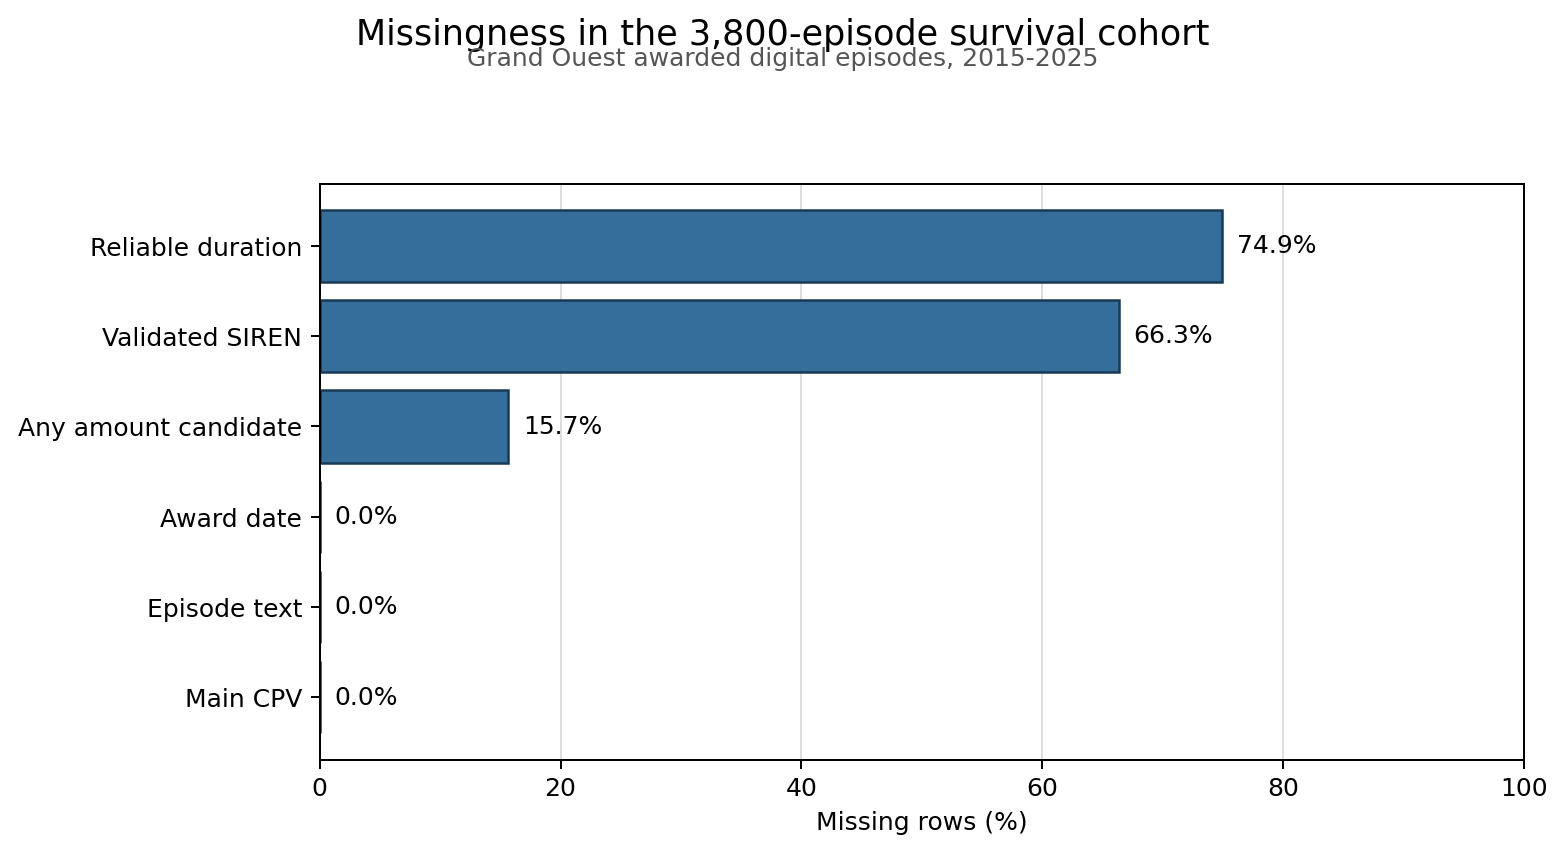
\includegraphics[width=0.8\linewidth]{figures/appB_missingness.png}
\caption{Completeness of the key cohort variables. Validated buyer identifiers and reliable durations are the
two fields whose absence shapes the methodology: the first forces a name-based fallback in buyer blocking,
the second rules out any duration-conditioned event definition.}
\label{fig:appb-missing}
\end{figure}

\begin{figure}[htbp]
\centering
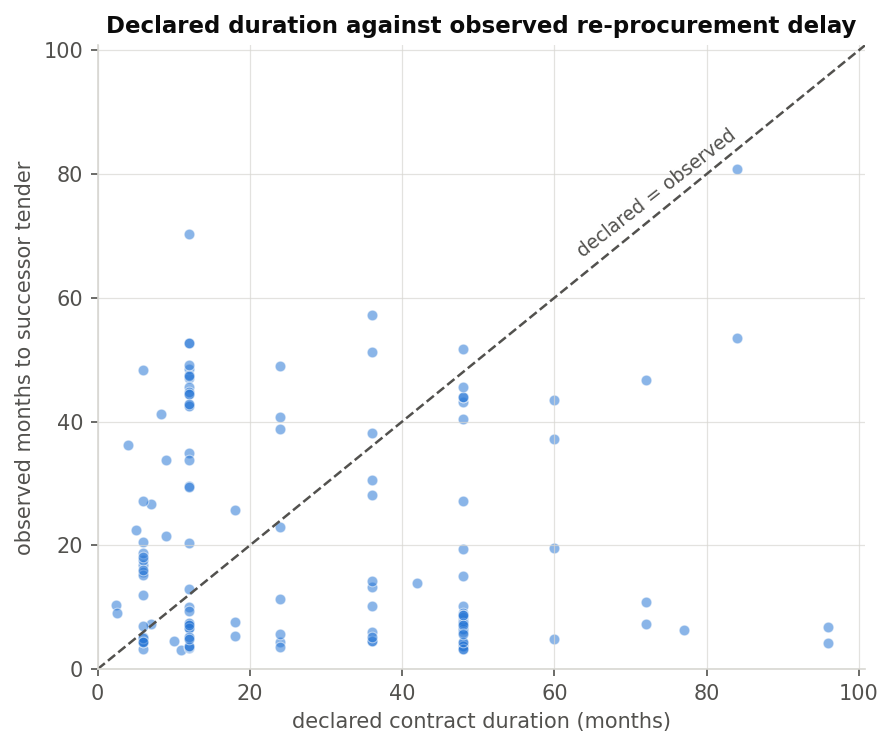
\includegraphics[width=0.8\linewidth]{figures/appB_duration_vs_observed.png}
\caption{Declared contract end against observed successor timing, for the episodes that carry both. Only
21.8\,\% of these contracts show an observable successor within six months of their declared end, and the
median absolute discrepancy is 21.1 months. This is the empirical basis for excluding declared duration from
the event definition rather than using it to bound the renewal window.}
\label{fig:appb-duration}
\end{figure}

\section{Linkage validation}
\label{app:linkage}

\subsection*{The regional reference}

A stratified review of 120 awarded digital anchors across Bretagne, Pays de la Loire and Normandie, carried
out on 11 August 2026 against the real BOAMP notices and their official URLs, before the linkage methods in
this project existed. 112 anchors re-resolve onto exactly one episode; 88 are usable. The pilot split holds
16 usable anchors (5 positive) and the locked split 72 (18 positive), with 5,221 and 20,917 candidate pair
rows respectively. The split is recorded in the reference file itself and is not post hoc.

Four limits bound its reach: the labels come from a single large-language-model research pass, spot-checked
rather than verified anchor by anchor; the per-anchor evidence trail was not recorded; negatives are
corpus-relative, because roughly 25 candidates per anchor were considered rather than the full pool; and the
rule that selected those 25 candidates was not recorded, so recall and the 0.913 candidate ceiling are not
fully independent of the score they bound. Precision is unaffected by the fourth limit.

\subsection*{Existence detection versus exact successor identity}

Two accountings answer different questions. Anchor-level accounting asks whether the system detected that a
successor exists. Exact-successor accounting asks whether it named the right one, so a wrong successor on a
positive anchor counts as one false positive \emph{and} one false negative. The project's headline figures
are the latter.

Method keys, as in the body: \texttt{M\_A} deterministic, \texttt{M\_B} text ranking (primary), \texttt{M\_C} weighted gated, \texttt{M\_D} Fellegi--Sunter.

\begin{longtable}[]{@{}lrrrrr@{}}
\toprule\noalign{}
Method (locked split) & Threshold & TP & FP & FN & TN \\
\midrule\noalign{}
\endhead
\multicolumn{6}{@{}l}{\emph{Existence detection (anchor level)}}\\
\texttt{M\_A} & n/a & 8 & 7 & 10 & 47 \\
\texttt{M\_B} & 0.70 & 8 & 0 & 10 & 54 \\
\texttt{M\_C} & 0.70 & 13 & 10 & 5 & 44 \\
\texttt{M\_D} & 0.65 & 4 & 1 & 14 & 53 \\
\midrule
\multicolumn{6}{@{}l}{\emph{Exact successor identity}}\\
\texttt{M\_A} & n/a & 8 & 7 & 10 & 47 \\
\texttt{M\_B} & 0.70 & 7 & 1 & 11 & 54 \\
\texttt{M\_C} & 0.70 & 12 & 11 & 6 & 44 \\
\texttt{M\_D} & 0.65 & 1 & 4 & 17 & 53 \\
\bottomrule\noalign{}
\end{longtable}

The gap between the two blocks is the whole point: \texttt{M\_C} detects five more anchors that do have a
successor, but names the wrong episode often enough that its exact-successor precision falls to 0.522.

\subsection*{Threshold sweep, \texttt{M\_B}, locked split}

\begin{longtable}[]{@{}rrrrrrr@{}}
\toprule\noalign{}
Threshold & Accepted & Correct & Precision & Recall & FPR & Coverage \\
\midrule\noalign{}
\endhead
0.50 & 21 & 10 & 0.476 & 0.556 & 0.167 & 0.292 \\
0.55 & 17 & 9 & 0.529 & 0.500 & 0.111 & 0.236 \\
0.60 & 13 & 9 & 0.692 & 0.500 & 0.056 & 0.181 \\
0.65 & 10 & 8 & 0.800 & 0.444 & 0.019 & 0.139 \\
\textbf{0.70} & \textbf{8} & \textbf{7} & \textbf{0.875} & \textbf{0.389} & \textbf{0.000} & \textbf{0.111} \\
0.75 & 7 & 6 & 0.857 & 0.333 & 0.000 & 0.097 \\
0.80 & 6 & 5 & 0.833 & 0.278 & 0.000 & 0.083 \\
\bottomrule\noalign{}
\end{longtable}

The row at 0.70 is the retained operating point. Git history records that the policy drew on inspection of
this designated locked stratum before the final pipeline was frozen. The table is therefore internal
validation and sensitivity evidence, not a fully untouched holdout. The operating point has not been moved
since, and the lower thresholds remain sensitivity arms rather than post-hoc replacements.

\begin{figure}[htbp]
\centering
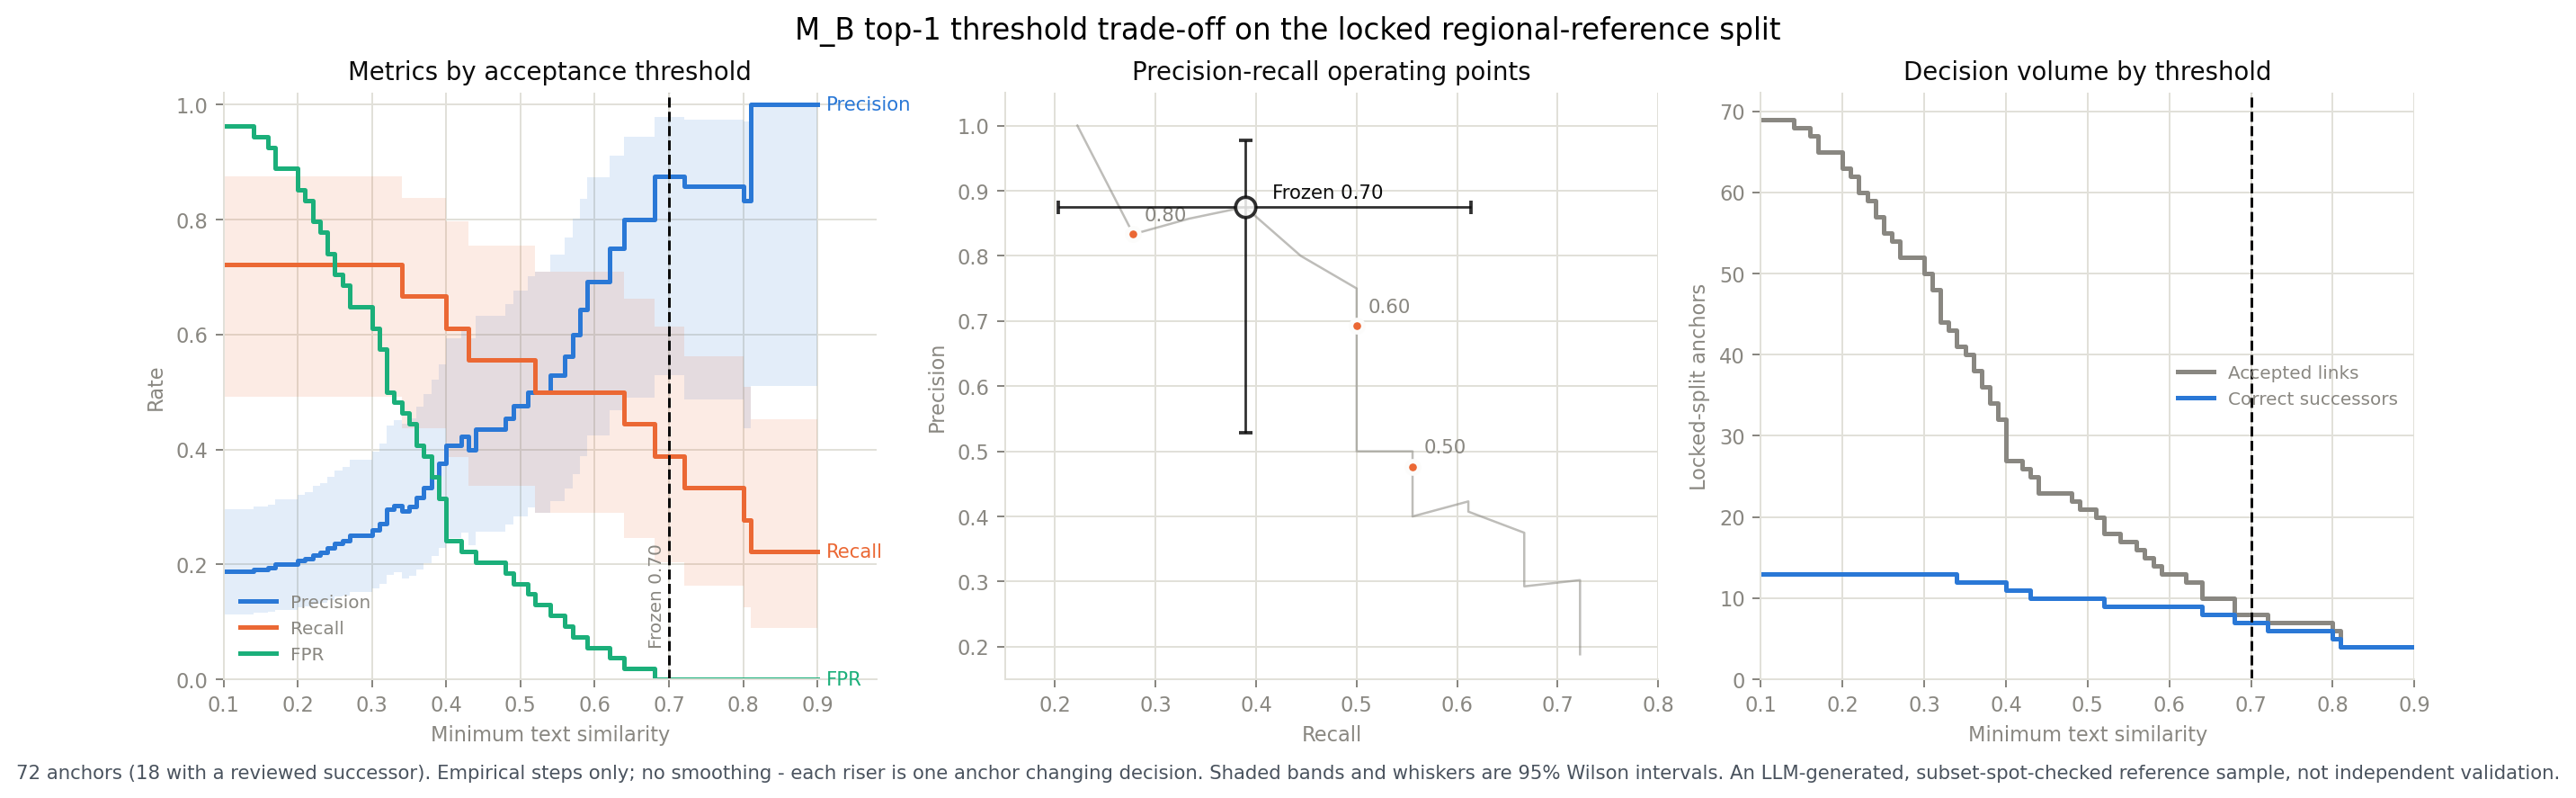
\includegraphics[width=\linewidth]{figures/fig05_threshold_tradeoff.png}
\caption{The complete threshold trade-off, all three panels. Left: precision, recall and false-positive rate against the acceptance threshold, with 95\,\% Wilson bands. Centre: the same information as precision--recall operating points, with the frozen 0.70 point and its interval marked. Right: how many anchors receive a link, and how many of those are the reviewed successor. The steps are empirical and unsmoothed: each riser is one anchor changing decision.}
\label{fig:appc-tradeoff}
\end{figure}

\subsection*{Pair-level ranking diagnostics}

\begin{longtable}[]{@{}lrrrr@{}}
\toprule\noalign{}
Method & ROC AUC & Average precision & Positive pairs & Negative pairs \\
\midrule\noalign{}
\endhead
\texttt{M\_A} & 0.7476 & 0.0378 & 16 & 20,901 \\
\texttt{M\_B} & 0.9915 & 0.4777 & 16 & 20,901 \\
\texttt{M\_C} & 0.9662 & 0.3452 & 16 & 20,901 \\
\texttt{M\_D} & 0.8383 & 0.0228 & 16 & 20,901 \\
\bottomrule\noalign{}
\end{longtable}

These curves rank scores; they do not measure accuracy at the acceptance threshold. The ROC AUC of 0.9915
does carry a real interpretation: on this internal reference, \texttt{M\_B} has a very high probability of
ranking a reviewed positive pair above a reviewed negative pair. With only 16 positive pairs among 20,917,
however, ROC AUC is less informative about the reliability of accepted positive links than precision--recall,
average precision and the anchor-level operating point \citep{davis2006,saito2015}. A second caveat applies to both: the 20,917 pairs come
from 69 anchors, so the observations are not independent and no clustered adjustment is made. The operating
point in the table above, not these curves, is what the event definition rests on.

\begin{figure}[htbp]
\centering
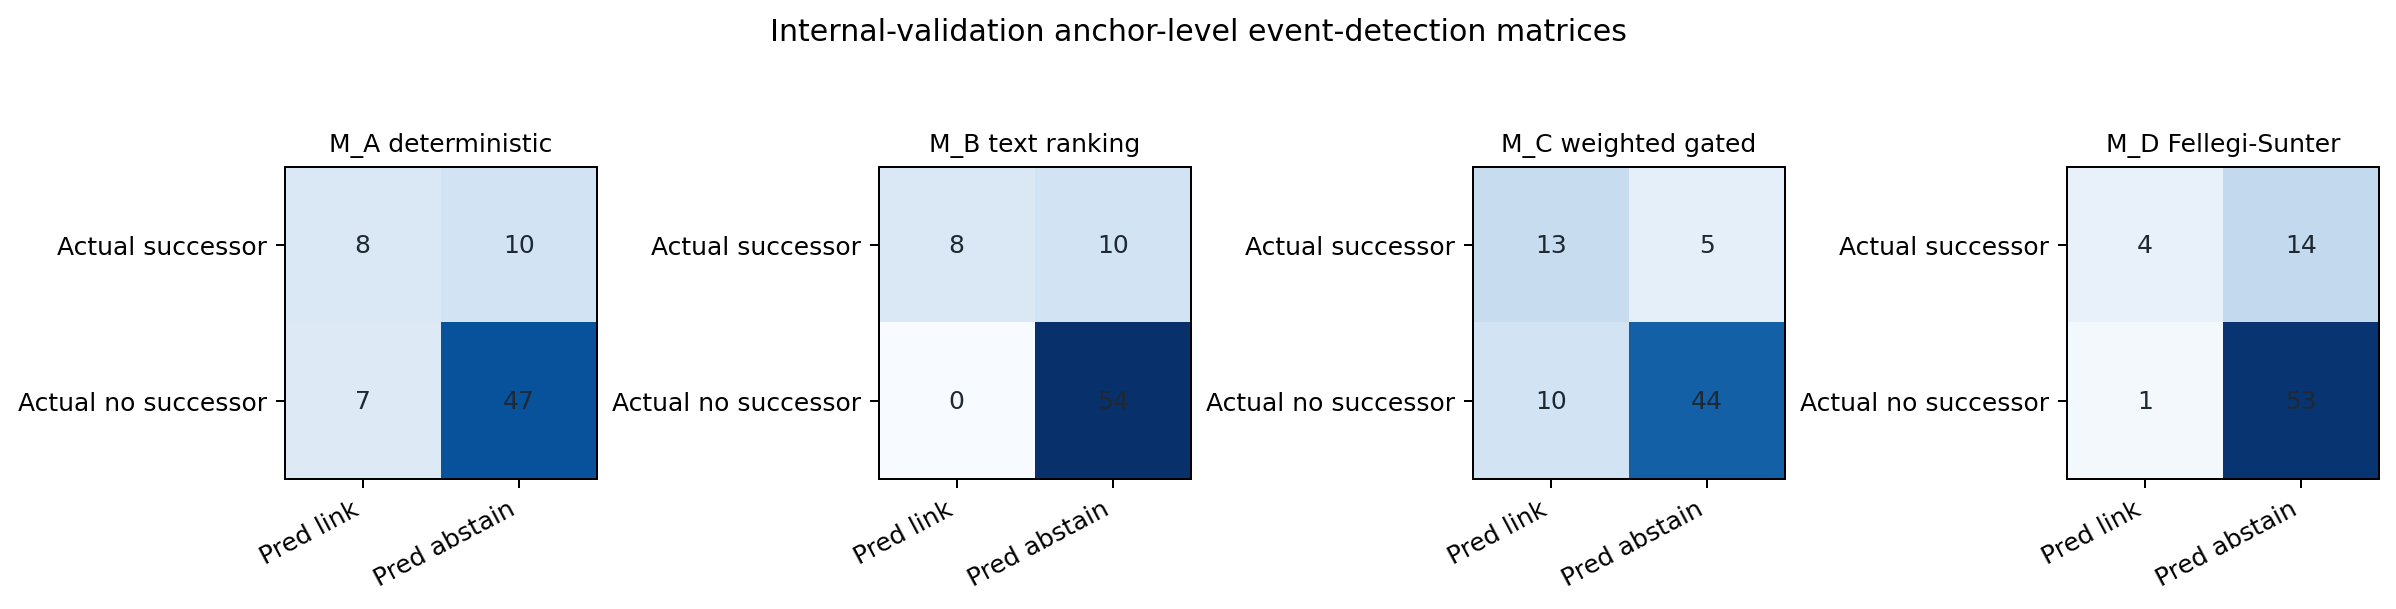
\includegraphics[width=0.9\linewidth]{figures/appC_confusion_matrices.png}
\caption{Anchor-level confusion matrices for the four linkage methods on the locked split. \texttt{M\_B} is
the only method with no accepted link on a reviewed-negative anchor; \texttt{M\_C} buys five additional
detections at the cost of ten.}
\label{fig:appc-cm}
\end{figure}

\begin{figure}[htbp]
\centering
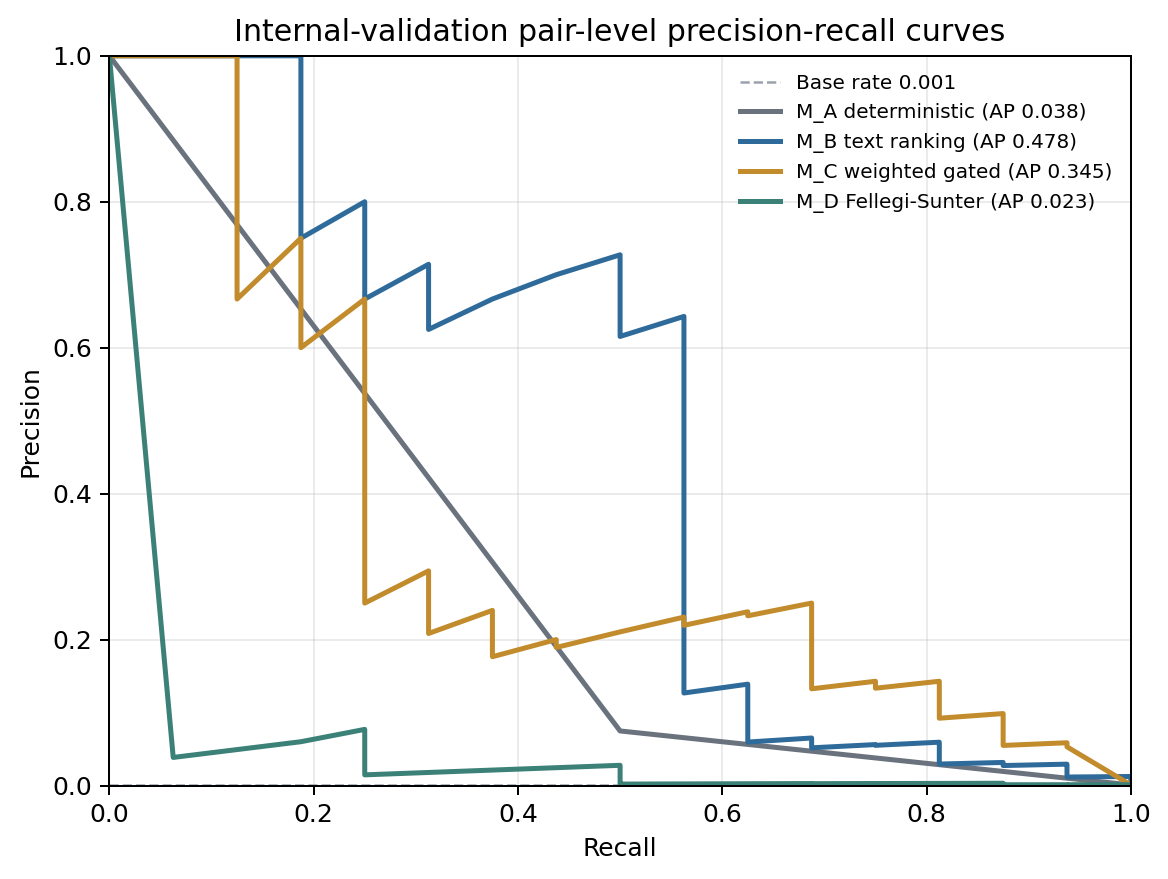
\includegraphics[width=0.72\linewidth]{figures/appC_pair_pr.png}
\caption{Pair-level precision--recall curves. The relevant diagnostic under extreme class imbalance, and the
one that shows how quickly precision degrades as recall is bought.}
\label{fig:appc-pr}
\end{figure}

\begin{figure}[htbp]
\centering
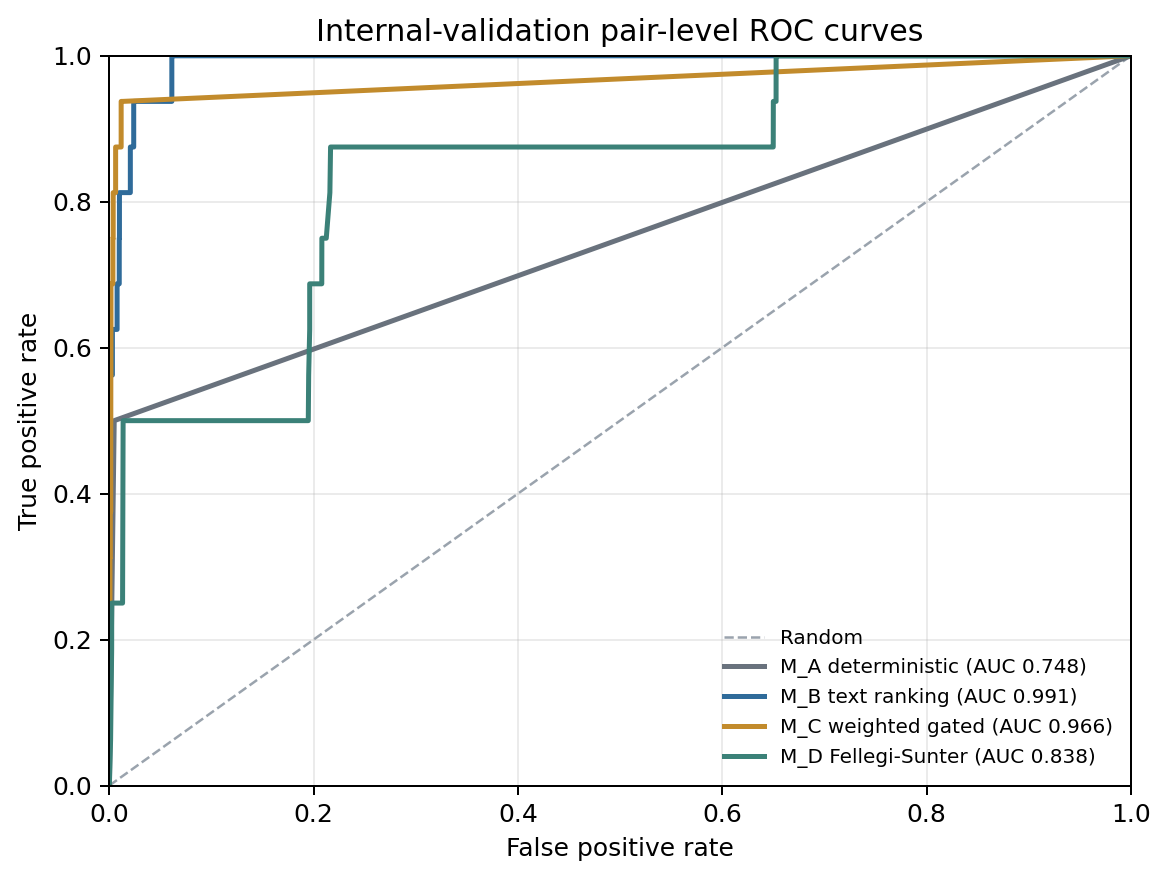
\includegraphics[width=0.72\linewidth]{figures/appC_pair_roc.png}
\caption{Pair-level ROC curves. \texttt{M\_B}'s AUC of 0.9915 indicates very strong pairwise ranking on the
internal reference. Under the 16-against-20,901 imbalance, precision--recall and anchor-level operating-point
metrics remain more decision-relevant for the reliability of accepted links.}
\label{fig:appc-roc}
\end{figure}

\subsection*{Candidate generation audit}

Candidate generation exposed 21 of the 23 reviewed successors, a pairs completeness of 0.913. Both
unreachable cases are attributed to a named blocking condition: one anchor never entered the cohort because
its award notice carries no structured Grand Ouest address, and one buyer changed legal form from CCAS to
CIAS with no shared SIREN. There are no unexplained cases, which is what separates an owned ceiling from an
implementation defect.

Of the 544 accepted links, 538 have a CPV division observed on both sides; 351 (65.2\,\%) stay within one
division. The reviewed reference successors cross divisions at a comparable rate, 9 of 23 (39.1\,\%), which
is why hard same-division blocking is not imposed: it would discard those 9 and cut the attainable recall
ceiling to 0.609. The buyer-blocking audit over the accepted links finds 0 conflicting validated SIRENs, 0
municipal / inter-municipal mixes, 18 name-only cross-department matches and 2 legal-family differences
flagged for review.

\subsection*{Challenge review}

A blinded 60-pair sample was prepared: 20 production-accepted links, 20 high-similarity structural negatives,
20 buyer-declared relationships, with a separate audit key and a pre-specified acceptance rule. The completed
review is model-assisted, not independent-human, and the repository records that provenance explicitly. Among
the 20 accepted links: 14 confirmed, 5 rejected, 1 uncertain, giving precision $14/19 = 0.737$ excluding the
uncertain row and $14/20 = 0.700$ on the conservative reading (exact 95\,\% interval $[0.457, 0.881]$). The
structural-negative stratum returned 19 negatives and 1 positive; the buyer-declared stratum 6 positives and
14 negatives, which demonstrates that a buyer-declared relationship is recruitment evidence rather than an
automatic successor label.

\section{Survival detail}
\label{app:survival}

\subsection*{Segment summary under the primary event definition}

\begin{longtable}[]{@{}lrrrrr@{}}
\toprule\noalign{}
Segment & Episodes & Events & Event rate & $S(12)$ & $S(24)$ \\
\midrule\noalign{}
\endhead
CPV-32 & 1,152 & 152 & 0.1319 & 0.9583 & 0.9400 \\
CPV-35 & 564 & 115 & 0.2039 & 0.9357 & 0.9043 \\
CPV-48 & 790 & 92 & 0.1165 & 0.9609 & 0.9323 \\
CPV-72 & 1,294 & 185 & 0.1430 & 0.9533 & 0.9391 \\
\bottomrule\noalign{}
\end{longtable}

Multivariate log-rank across the four segments: statistic 23.45, $p = 3.26 \times 10^{-5}$.

\subsection*{Cox model, full output}

\begin{longtable}[]{@{}>{\raggedright\arraybackslash}p{4.6cm}rrrr@{}}
\toprule\noalign{}
Covariate & $\hat\beta$ & HR & 95\,\% CI & $p$ \\
\midrule\noalign{}
\endhead
Framework agreement & 0.5600 & 1.751 & [1.435, 2.136] & $3.38\times 10^{-8}$ \\
Validated SIREN & 0.0787 & 1.082 & [0.885, 1.323] & 0.443 \\
Award year (centred) & 0.1016 & 1.107 & [1.066, 1.149] & $1.21\times 10^{-7}$ \\
CPV-35 (ref. CPV-32) & 0.4405 & 1.553 & [1.218, 1.981] & $3.83\times 10^{-4}$ \\
CPV-48 & $-0.1892$ & 0.828 & [0.638, 1.073] & 0.153 \\
CPV-72 & 0.0540 & 1.056 & [0.850, 1.310] & 0.624 \\
Normandie (ref. Bretagne) & $-0.2230$ & 0.800 & [0.640, 1.000] & 0.050 \\
Pays de la Loire & 0.0028 & 1.003 & [0.815, 1.234] & 0.979 \\
\bottomrule\noalign{}
\end{longtable}

3,800 awarded procurement episodes, 544 events, 8 covariates, partial AIC 8,537.99, in-sample concordance 0.6257.

\subsection*{Proportional-hazards diagnostics}

\begin{longtable}[]{@{}>{\raggedright\arraybackslash}p{6.5cm}rr@{}}
\toprule\noalign{}
Covariate & Test statistic & $p$ \\
\midrule\noalign{}
\endhead
Award year (centred) & 70.73 & $4.09\times 10^{-17}$ \\
Framework agreement & 7.04 & 0.0080 \\
Validated SIREN & 6.76 & 0.0093 \\
CPV-72 & 3.72 & 0.0537 \\
Pays de la Loire & 2.45 & 0.117 \\
Normandie (ref. Bretagne) & 0.61 & 0.436 \\
CPV-48 & 0.67 & 0.413 \\
CPV-35 (ref. CPV-32) & 0.04 & 0.840 \\
\bottomrule\noalign{}
\end{longtable}

Three covariates reject the constant-effect null. The award-year violation is severe and structurally
expected, because award year is confounded with follow-up length. \emph{The two segment coefficients that
carry the report's comparative claims are the two that pass the diagnostic most comfortably.}

\subsection*{Parametric family comparison}

\begin{longtable}[]{@{}lrrrr@{}}
\toprule\noalign{}
Family & Parameters & Log-likelihood & AIC & BIC \\
\midrule\noalign{}
\endhead
Generalised gamma & 3 & $-3{,}757.49$ & \textbf{7,520.99} & \textbf{7,539.72} \\
Log-normal & 2 & $-3{,}784.62$ & 7,573.24 & 7,585.73 \\
Log-logistic & 2 & $-3{,}807.28$ & 7,618.57 & 7,631.05 \\
Weibull & 2 & $-3{,}814.68$ & 7,633.35 & 7,645.84 \\
Exponential & 1 & $-3{,}829.66$ & 7,661.31 & 7,667.55 \\
\bottomrule\noalign{}
\end{longtable}

\begin{figure}[htbp]
\centering
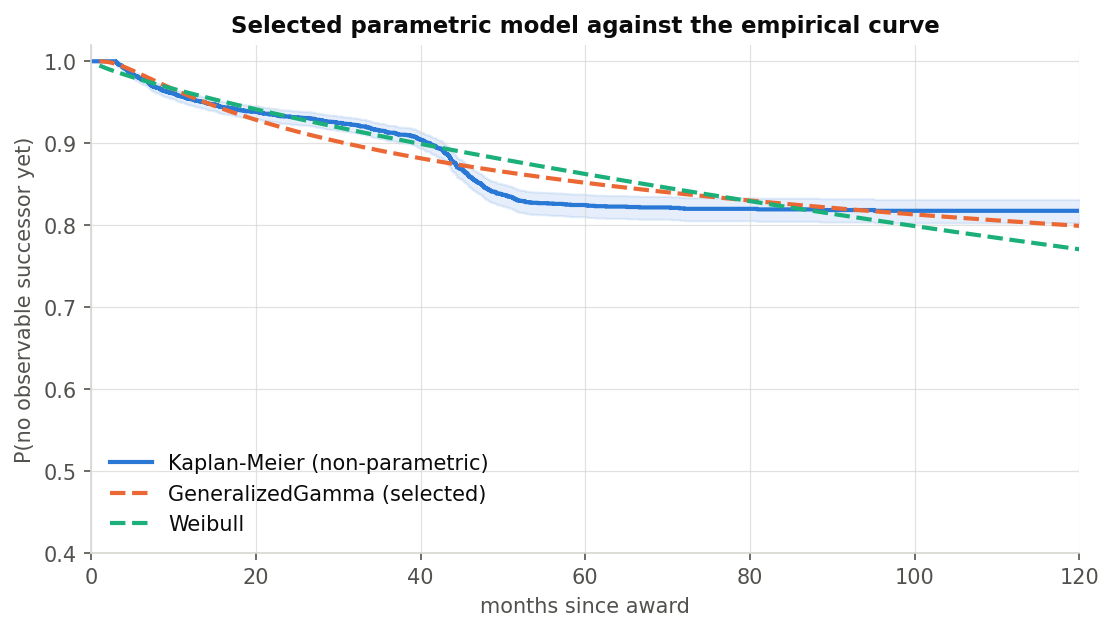
\includegraphics[width=0.8\linewidth]{figures/appD_parametric_vs_empirical.png}
\caption{Fitted parametric survival functions against the empirical Kaplan--Meier curve. Every smooth family
flattens the observed 36--48 month re-procurement shoulder, which is precisely the feature of operational interest. This is
why the reported 12- and 24-month probabilities are read off the empirical estimator, even though the
generalised gamma has the lowest AIC and BIC.}
\label{fig:appd-param}
\end{figure}

\subsection*{Sensitivity arms}

\begin{longtable}[]{@{}>{\raggedright\arraybackslash}p{3.4cm}rrrrr@{}}
\toprule\noalign{}
Arm & Events & Rate & $P(\le 12\text{m})$ & $P(\le 24\text{m})$ & Median observed gap \\
\midrule\noalign{}
\endhead
\texttt{M\_B @ 0.80} strict & 296 & 0.0779 & 2.37\,\% & 3.23\,\% & 35.7 m \\
\texttt{M\_B @ 0.70} primary & 544 & 0.1432 & 4.62\,\% & 6.73\,\% & 31.8 m \\
\texttt{M\_B @ 0.60} loose & 853 & 0.2245 & 8.00\,\% & 11.47\,\% & 26.6 m \\
\texttt{M\_C @ 0.70} contrast & 1,332 & 0.3505 & 12.21\,\% & 17.98\,\% & 26.1 m \\
\bottomrule\noalign{}
\end{longtable}

\subsection*{Buyer-stratified Cox sensitivity}
Robust score-based inference is one way to address clustered Cox data \citep{linwei1989}; the sensitivity here instead changes the estimand by stratifying on buyer and estimating effects only from within-buyer comparisons.

The primary within-buyer model contains 2,188 episodes, 511 events and 195 buyers. Each buyer receives its own
baseline hazard, so fixed buyer characteristics are absorbed. Candidate-pool size is not: it varies within 473
of the 514 buyers carrying multiple cohort episodes.

\begin{longtable}[]{@{}>{\raggedright\arraybackslash}p{5.2cm}rrr@{}}
\toprule\noalign{}
Covariate & HR & 95\,\% CI & $p$ \\
\midrule\noalign{}
\endhead
Framework agreement & 1.497 & [1.150, 1.948] & 0.0027 \\
Award year (centred) & 1.015 & [0.967, 1.065] & 0.547 \\
CPV-35 (ref. CPV-32) & 1.213 & [0.866, 1.699] & 0.262 \\
CPV-48 & 0.482 & [0.346, 0.672] & $1.7\times10^{-5}$ \\
CPV-72 & 0.831 & [0.627, 1.100] & 0.196 \\
\bottomrule\noalign{}
\end{longtable}

Across the four linkage arms, the CPV-35 estimates are 1.265, 1.213, 1.280 and 1.109; the CPV-48 estimates
are 0.477, 0.482, 0.589 and 0.744; and the framework estimates are 1.128, 1.497, 1.664 and 1.459. Directional
stability is distinct from significance in every arm: the strict framework estimate is imprecise.

\begingroup
\setlength{\tabcolsep}{4.5pt}
\begin{longtable}[]{@{}>{\raggedright\arraybackslash}p{5.4cm}rrrrr@{}}
\toprule\noalign{}
Robustness check & Episodes & Events & $P(\le 12\text{m})$ & CPV-35 HR & Framework HR \\
\midrule\noalign{}
\endhead
Main & 3,800 & 544 & 4.62\,\% & 1.553 & 1.751 \\
Excluding the borderline band $[0.65,0.75]$ & 3,520 & 411 & 3.72\,\% & 1.780 & 1.616 \\
Re-censoring template-risk links & 3,800 & 371 & 2.64\,\% & 1.541 & 1.692 \\
\bottomrule\noalign{}
\end{longtable}
\endgroup

The borderline band removes 280 episodes, of which 133 are events and 147 censored. The template-risk check
re-censors 173 of the 544 accepted links (31.8\,\%): 65 carry word-level similarity below 0.50, and 127 share
their successor episode with another anchor.

\subsection*{Detectability diagnostic}

\begin{longtable}[]{@{}>{\raggedright\arraybackslash}p{5.6cm}rrr@{}}
\toprule\noalign{}
Variable & Linked mean & Censored mean & SMD \\
\midrule\noalign{}
\endhead
log(candidate pool size) & 4.787 & 3.972 & $+0.470$ \\
Candidate pool size & 274.3 & 188.6 & $+0.285$ \\
Episode text length & 1,611 & 1,087 & $+0.262$ \\
Framework agreement & 0.2647 & 0.1867 & $+0.187$ \\
Administrative follow-up (months) & 70.65 & 65.38 & $+0.146$ \\
Award year & 2020 & 2020 & $-0.137$ \\
Validated SIREN & 0.3107 & 0.3409 & $-0.065$ \\
Notices per episode & 1.978 & 2.045 & $-0.058$ \\
Reliable duration present & 0.2445 & 0.2518 & $-0.017$ \\
\bottomrule\noalign{}
\end{longtable}

Sensitivity model adding $\log(1 + \text{pool size})$ to the main specification:

\begin{longtable}[]{@{}>{\raggedright\arraybackslash}p{5.0cm}rrr@{}}
\toprule\noalign{}
Covariate & HR, main & HR, adjusted & $p$, adjusted \\
\midrule\noalign{}
\endhead
Framework agreement & 1.751 & 1.617 & $2.6\times 10^{-6}$ \\
Validated SIREN & 1.082 & 0.983 & 0.87 \\
Award year (centred) & 1.107 & 1.145 & $4.1\times 10^{-11}$ \\
CPV-35 (ref. CPV-32) & 1.553 & 1.512 & $8.5\times 10^{-4}$ \\
CPV-48 & 0.828 & 0.769 & 0.048 \\
CPV-72 & 1.056 & 0.977 & 0.83 \\
Normandie (ref. Bretagne) & 0.800 & 0.796 & 0.046 \\
Pays de la Loire & 1.003 & 0.975 & 0.81 \\
log(candidate pool size) & --- & 1.184 & $6.0\times 10^{-9}$ \\
\bottomrule\noalign{}
\end{longtable}

\subsection*{Segment-stratified watch list}

The one operational artifact derived from these curves is a segment-stratified list: for each of the four CPV
segments, the five still-unlinked episodes awarded in 2021 or later with the highest conditional probability
of showing a successor within twelve months. It is read off the segment-stratified Kaplan--Meier curves, not
off the Cox model, and it is stratified deliberately. Because the conditional probability is a function of
segment and age alone, an unstratified ranking would simply return the highest-hazard segment at the age
closest to the shoulder, implying an individual-level precision that the out-of-time concordance of 0.479
does not support. The file is
\texttt{data/processed/boamp/segment\_watch\_km.csv}.

\section{Technology classification detail}
\label{app:nlp}

\subsection*{Annotated corpus}

500 manually annotated BOAMP notices, 2015--2025, all with a non-empty object text, no duplicate identifiers.
The sample is quota-stratified, so the class shares below are a property of the annotation design and are not
prevalence estimates.

\begin{longtable}[]{@{}lrr@{}}
\toprule\noalign{}
Class & $n$ & Share \\
\midrule\noalign{}
\endhead
BUSINESS\_SOFTWARE & 88 & 0.176 \\
NETWORK\_TELECOM & 81 & 0.162 \\
IT\_SERVICES & 74 & 0.148 \\
CYBERSECURITY & 54 & 0.108 \\
OTHER\_DIGITAL & 53 & 0.106 \\
IT\_INFRASTRUCTURE & 46 & 0.092 \\
CLOUD\_HOSTING & 32 & 0.064 \\
DATA\_BI & 29 & 0.058 \\
MIXED & 21 & 0.042 \\
OTHER & 15 & 0.030 \\
AI & 7 & 0.014 \\
\bottomrule\noalign{}
\end{longtable}

451 of the 500 notices are in the Grand Ouest and all 500 carry a digital CPV; 434 are tender notices, 55
award notices and 9 corrections. Only 243 belong to cohort episodes, so performance measured on this corpus
is evidence about the corpus rather than about the deployment population.

\subsection*{Specification comparison}

All six specifications share identical group-aware folds and an identical inner search budget.

\begingroup
\small
\setlength{\tabcolsep}{4pt}
\begin{longtable}[]{@{}llrr@{}}
\toprule\noalign{}
Model & Features & CV macro-F1 (SD) & Out-of-fold macro-F1 \\
\midrule\noalign{}
\endhead
\texttt{M\_majority} & --- & 0.027 (0.000) & --- \\
\texttt{M0\_cpv} & CPV tokens & 0.439 (0.076) & 0.441 \\
\texttt{M0b\_cpv\_descriptor} & CPV + descriptors & 0.469 (0.038) & 0.473 \\
\texttt{M1\_tfidf\_logreg} & object text & 0.662 (0.067) & 0.670 \\
\textbf{\texttt{M2\_tfidf\_logreg\_balanced}} & object text & \textbf{0.741 (0.034)} & \textbf{0.744} \\
\texttt{M3\_tfidf\_linearsvm} & object text & 0.717 (0.030) & 0.718 \\
\texttt{M4\_tfidf\_linearsvm\_balanced} & object text & 0.716 (0.054) & 0.715 \\
\bottomrule\noalign{}
\end{longtable}
\endgroup

Two aggregations appear above and should not be confused: the CV column averages the three fold scores, while
the out-of-fold column computes one score over the pooled 500 held-out predictions.

\subsection*{Per-class performance, out of fold}

\begin{longtable}[]{@{}lrrrrr@{}}
\toprule\noalign{}
Class & Precision & Recall & F1 & Support & Predicted \\
\midrule\noalign{}
\endhead
DATA\_BI & 0.923 & 0.828 & 0.873 & 29 & 26 \\
OTHER & 0.923 & 0.800 & 0.857 & 15 & 13 \\
BUSINESS\_SOFTWARE & 0.798 & 0.898 & 0.845 & 88 & 99 \\
NETWORK\_TELECOM & 0.810 & 0.840 & 0.824 & 81 & 84 \\
CYBERSECURITY & 0.848 & 0.722 & 0.780 & 54 & 46 \\
IT\_SERVICES & 0.778 & 0.757 & 0.767 & 74 & 72 \\
IT\_INFRASTRUCTURE & 0.702 & 0.717 & 0.710 & 46 & 47 \\
OTHER\_DIGITAL & 0.655 & 0.679 & 0.667 & 53 & 55 \\
AI & 0.800 & 0.571 & \emph{0.667} & \emph{7} & 5 \\
CLOUD\_HOSTING & 0.731 & 0.594 & 0.655 & 32 & 26 \\
MIXED & 0.482 & 0.619 & 0.542 & 21 & 27 \\
\bottomrule\noalign{}
\end{longtable}

The \texttt{AI} row is printed with its support and marked unevaluable: an F1 of 0.667 on seven annotated
notices rests on three correct predictions, and both a high and a low value would be uninformative.

\subsection*{Error triage}

Thirty representative out-of-fold errors were sampled from the largest confusion pairs: 16 model errors,
7 taxonomy-boundary ambiguities, 4 genuinely multi-technology procurements, 2 annotation inconsistencies in
related notices, 1 object text too poor to decide. Close to half the residual therefore comes from class
definitions or missing information rather than from model capacity --- which is also why a larger model was
not the indicated remedy.

\subsection*{Temporal robustness}

Training 2015--2022 ($n = 393$), test 2023--2025 ($n = 107$), with the four boundary-straddling families
assigned to training in full. All-class macro-F1 0.662; macro-F1 over the five classes with test support of
at least 10 (\texttt{CYBERSECURITY}, \texttt{NETWORK\_TELECOM}, \texttt{BUSINESS\_SOFTWARE},
\texttt{IT\_SERVICES}, \texttt{OTHER\_DIGITAL}) is 0.815; weighted F1 0.772; accuracy 0.776.

\subsection*{Deployed confidence: reliability out of fold}

\begin{longtable}[]{@{}lrrrr@{}}
\toprule\noalign{}
Stated confidence & $n$ & Observed accuracy & Mean stated & Gap \\
\midrule\noalign{}
\endhead
$[0.0,0.3)$ & 151 & 0.523 & 0.224 & $+0.299$ \\
$[0.3,0.4)$ & 114 & 0.825 & 0.349 & $+0.476$ \\
$[0.4,0.5)$ & 91 & 0.813 & 0.454 & $+0.359$ \\
$[0.5,0.6)$ & 57 & 0.983 & 0.544 & $+0.438$ \\
$[0.6,0.7)$ & 42 & 0.905 & 0.653 & $+0.252$ \\
$[0.7,0.8)$ & 26 & 0.962 & 0.735 & $+0.227$ \\
$[0.8,0.9)$ & 16 & 0.938 & 0.854 & $+0.084$ \\
$[0.9,1.0)$ & 3 & 1.000 & 0.938 & $+0.062$ \\
\bottomrule\noalign{}
\end{longtable}

The gap is positive in every bin above 0.3: the score understates its own hit rate. Expected calibration
error of the deployed variant is 0.350. Platt scaling cut that error by 0.1405 --- clearing the 0.02
requirement --- but cost 0.0364 macro-F1, exceeding the 0.02 budget, so the pre-specified rule rejected it and
the rule was not relaxed.

Cohort coverage by cutoff: 648 episodes at $\ge 0.5$, 412 at $\ge 0.6$, 235 at $\ge 0.7$, 123 at $\ge 0.8$,
28 at $\ge 0.9$; the highest deployed confidence is 0.9707.

\subsection*{Downstream eligibility}

\begin{longtable}[]{@{}lrrrll@{}}
\toprule\noalign{}
Class & CV F1 & Episodes & Events & Gate A & Gate B \\
\midrule\noalign{}
\endhead
CYBERSECURITY & 0.780 & 316 & 60 & pass & pass \\
NETWORK\_TELECOM & 0.824 & 859 & 140 & pass & pass \\
IT\_INFRASTRUCTURE & 0.710 & 298 & 38 & pass & pass \\
BUSINESS\_SOFTWARE & 0.845 & 854 & 106 & pass & pass \\
IT\_SERVICES & 0.767 & 492 & 72 & pass & pass \\
CLOUD\_HOSTING & 0.655 & 115 & 11 & pass & fail \\
DATA\_BI & 0.873 & 86 & 15 & pass & fail \\
AI & 0.667 & 6 & 0 & fail & fail \\
MIXED & 0.542 & 139 & 32 & fail & pass \\
OTHER\_DIGITAL & 0.667 & 462 & 44 & fail & pass \\
OTHER & 0.857 & 173 & 26 & fail & pass \\
\bottomrule\noalign{}
\end{longtable}

Gate A requires a substantive technology class with annotated support $\ge 10$ and out-of-fold F1 $\ge 0.65$;
Gate B requires $\ge 100$ episodes and $\ge 20$ events. Applying Gate A moves the technology log-rank result
from $p = 0.000119$ (8 classes, 518 events) to $p = 0.0363$ (5 classes, 416 events). The gate costs
significance and was kept.

\begin{figure}[htbp]
\centering
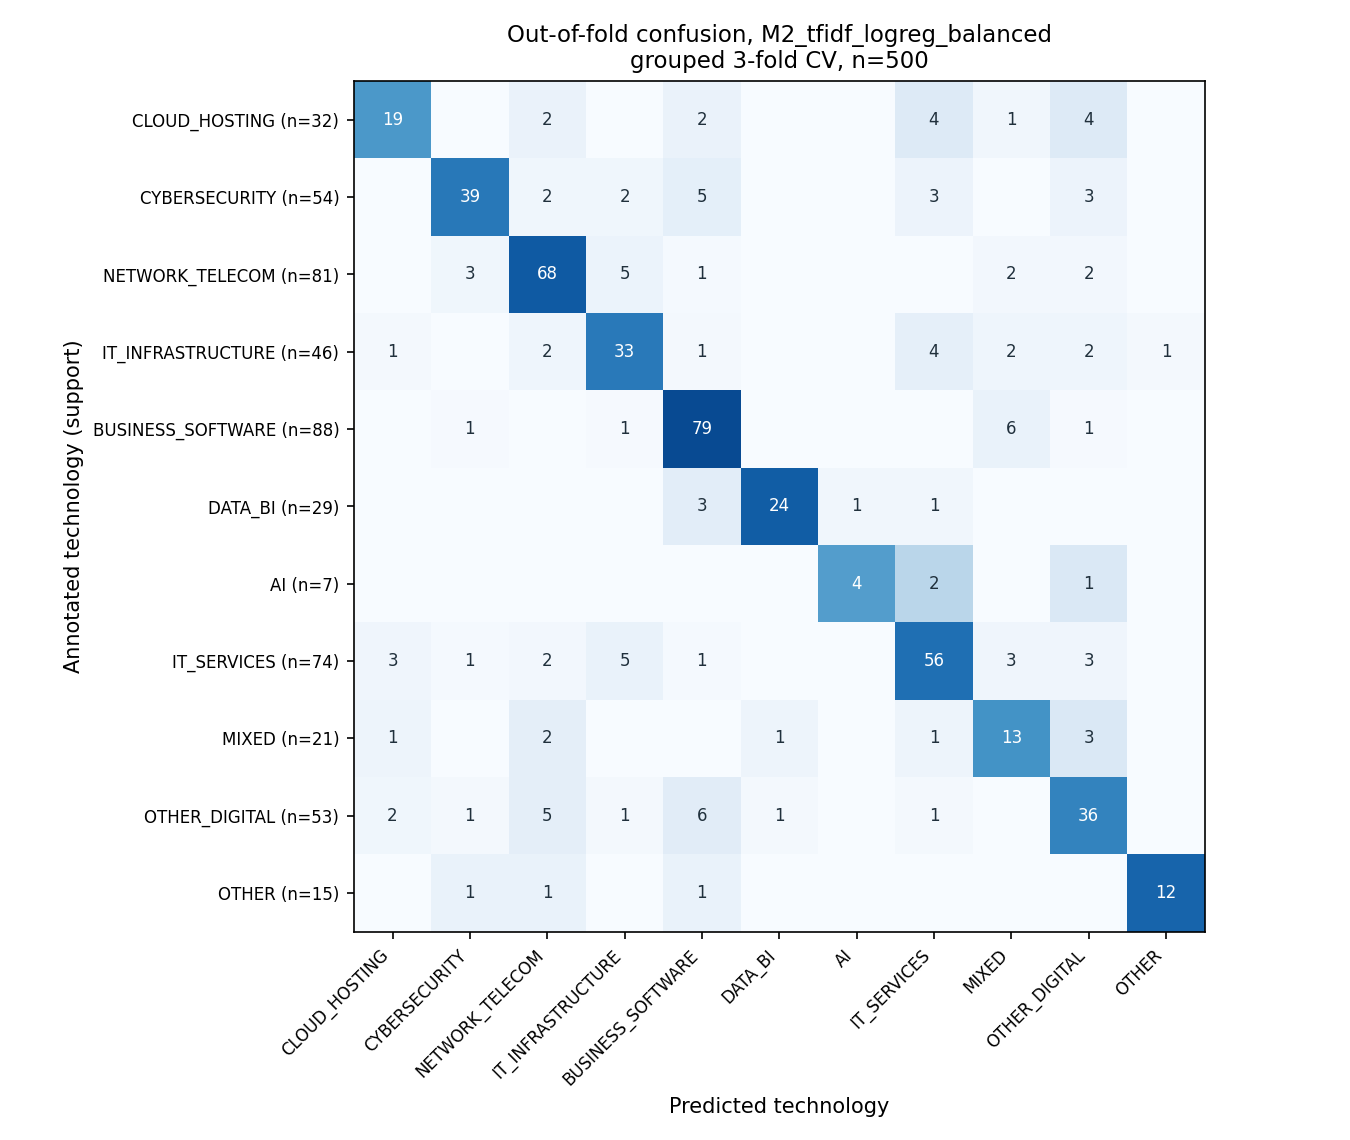
\includegraphics[width=0.85\linewidth]{figures/appE_tech_confusion.png}
\caption{Out-of-fold confusion matrix over the eleven classes. The dominant confusions run along definitional
boundaries --- \texttt{OTHER\_DIGITAL} against \texttt{BUSINESS\_SOFTWARE} and \texttt{NETWORK\_TELECOM},
\texttt{IT\_SERVICES} against \texttt{IT\_INFRASTRUCTURE} --- rather than being spread at random.}
\label{fig:appe-cm}
\end{figure}

\begin{figure}[htbp]
\centering
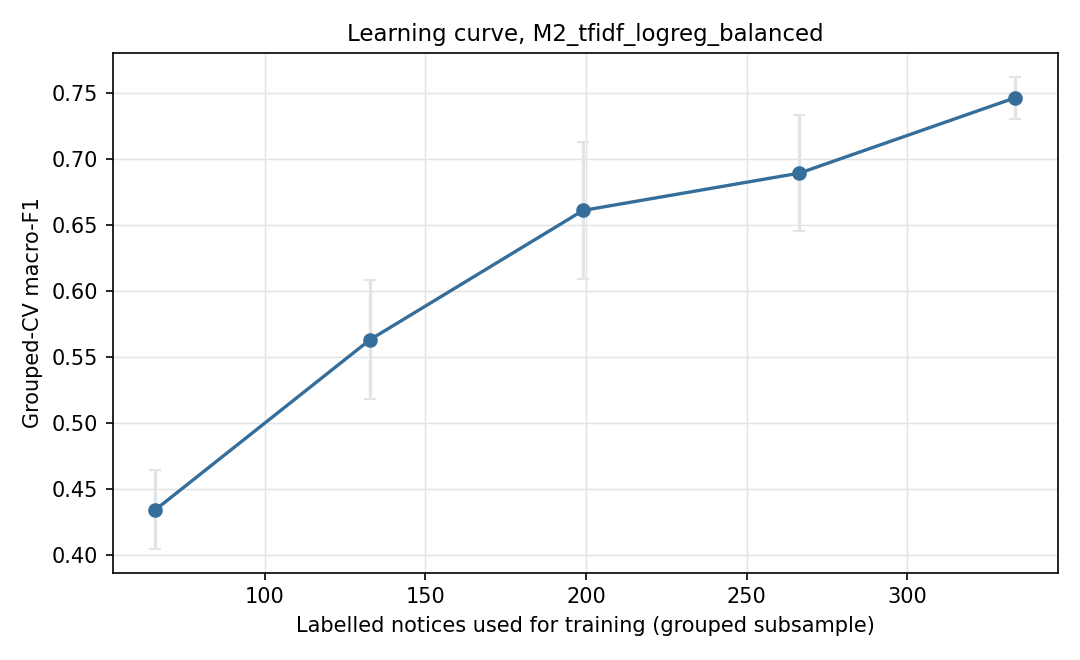
\includegraphics[width=0.72\linewidth]{figures/appE_learning_curve.png}
\caption{Learning curve, subsampling procurement \emph{families} rather than notices. Training F1 sits near
0.99 at every size while validation F1 climbs from 0.434 to 0.747 and has not flattened at $n = 500$. This is
a variance-limited regime: more annotation is the indicated remedy, not more model capacity --- which is the
diagnostic behind the decision not to run a transformer.}
\label{fig:appe-lc}
\end{figure}

\begin{figure}[htbp]
\centering
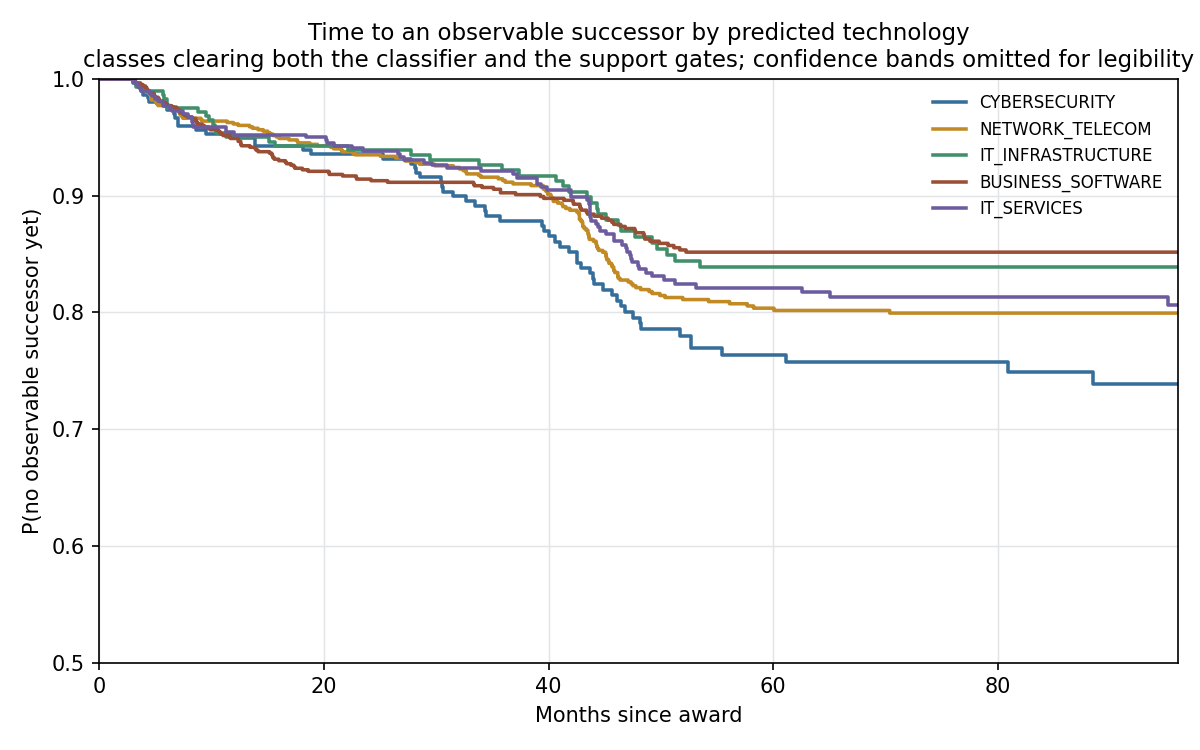
\includegraphics[width=0.78\linewidth]{figures/appE_technology_km.png}
\caption{Kaplan--Meier curves for the five predicted technology classes clearing both Gate A (classifier
quality) and Gate B (downstream statistical support). Confidence bands are omitted for legibility; the axis
starts at 0.5.}
\label{fig:appe-km}
\end{figure}

\section{Trend detail}
\label{app:trend}

\subsection*{Signal matrix}

\begin{longtable}[]{@{}lrrrrl@{}}
\toprule\noalign{}
Segment & Slope & Raw $p$ & Holm $p$ & BH $p$ & Reading \\
\midrule\noalign{}
\endhead
Overall & $-0.11$ & 0.921 & 1.000 & 0.989 & no signal \\
CPV-32 & $-0.01$ & 0.989 & 1.000 & 0.989 & no signal \\
CPV-35 & $+0.03$ & 0.923 & 1.000 & 0.989 & no signal \\
CPV-48 & $-0.84$ & \textbf{0.032} & 0.159 & 0.159 & nominal signal only \\
CPV-72 & $+0.70$ & 0.285 & 1.000 & 0.714 & no signal \\
\bottomrule\noalign{}
\end{longtable}

Slopes are ordinary least squares over the last twelve quarters, in awarded episodes per quarter. Five series
are tested simultaneously, so raw $p$-values are reported beside Holm and Benjamini--Hochberg adjustments. The
pre-declared exploratory level is $\alpha = 0.10$ on the raw $p$-value, fixed before the series were fitted
and left unchanged.

\subsection*{PELT change points under three penalties}

\begin{longtable}[]{@{}llll@{}}
\toprule\noalign{}
Segment & Candidate breaks ($\lambda = 0.5$) & $\lambda = 1$ & $\lambda = 2$ \\
\midrule\noalign{}
\endhead
Overall & 2020Q4, 2023Q2 & 2023Q2 & --- \\
CPV-32 & 2020Q2 & 2020Q2 & 2020Q2 \\
CPV-35 & 2019Q1, 2020Q2, 2022Q3 & 2019Q1, 2020Q2 & 2022Q3 \\
CPV-48 & 2024Q1 & 2024Q1 & 2024Q1 \\
CPV-72 & 2021Q1, 2023Q1 & 2021Q1, 2023Q1 & 2021Q1 \\
\bottomrule\noalign{}
\end{longtable}

The penalty is the only tuning knob, and it trades a better fit against more breaks; the practical consequences are reviewed by \citet{truong2020}. A break is called \emph{stable} only when a break lies within one quarter under all three penalties. Three
qualify: CPV-32 at 2020Q2, CPV-48 at 2024Q1, CPV-72 at 2021Q1. The overall series and CPV-35 carry none: their
candidates disappear as soon as the penalty changes. No break is attributed to a cause; PELT dates a level
shift, it does not explain one.

\subsection*{Stationarity}

\begin{longtable}[]{@{}lrrrr@{}}
\toprule\noalign{}
Segment & ADF statistic & ADF $p$ & KPSS statistic & KPSS $p$ \\
\midrule\noalign{}
\endhead
Overall & $-5.890$ & 0.000 & 0.268 & 0.100 \\
CPV-32 & $-6.086$ & 0.000 & 0.808 & 0.010 \\
CPV-35 & $-1.684$ & 0.439 & 0.444 & 0.058 \\
CPV-48 & $-1.749$ & 0.406 & 0.545 & 0.032 \\
CPV-72 & $-5.439$ & 0.000 & 0.611 & 0.022 \\
\bottomrule\noalign{}
\end{longtable}

The two tests carry opposite nulls --- ADF assumes a unit root, KPSS assumes level stationarity --- so they are
read together. Only the overall series gives a clean reading (rejects the unit root, fails to reject
stationarity). The others disagree, which means the series is not cleanly classified over a window this short.
That ambiguity is reported rather than resolved, and nothing in the report depends on resolving it.

\subsection*{Regime model}

\begin{longtable}[]{@{}llrl@{}}
\toprule\noalign{}
Segment & Current regime & Posterior & Mean quarterly change by regime \\
\midrule\noalign{}
\endhead
Overall & growth & 0.750 & decline $-15.5$, plateau $-7.8$, growth $+17.8$ \\
CPV-32 & growth & 0.992 & decline $-12.3$, plateau $-0.5$, growth $+11.6$ \\
CPV-72 & growth & 0.594 & decline $-6.6$, plateau $+0.1$, growth $+7.5$ \\
\bottomrule\noalign{}
\end{longtable}

The three-state Gaussian hidden Markov model is fitted on the quarter-over-quarter \emph{change} in episode
count, not on the level, so its states describe a typical direction of movement rather than a segment's
activity. Because the series are noisy and low-count, the \texttt{plateau} state is a data-driven middle tier
rather than a change centred exactly at zero. A regime label is a model belief about the most recent quarter;
the twelve-quarter slope summarises a different window, and the two need not agree.

\subsection*{Technology series}

\begin{longtable}[]{@{}lrrrrl@{}}
\toprule\noalign{}
Class & Episodes & Slope & Raw $p$ & Holm $p$ & Reading \\
\midrule\noalign{}
\endhead
NETWORK\_TELECOM & 855 & $-0.255$ & 0.515 & 1.000 & no trend detected \\
CYBERSECURITY & 314 & $+0.196$ & 0.463 & 1.000 & no trend detected \\
BUSINESS\_SOFTWARE & 849 & $-0.762$ & 0.248 & 0.992 & no trend detected \\
IT\_INFRASTRUCTURE & 295 & $-0.018$ & 0.901 & 1.000 & no trend detected \\
IT\_SERVICES & 486 & $+0.448$ & 0.194 & 0.972 & no trend detected \\
\bottomrule\noalign{}
\end{longtable}

Technology and CPV series now use the same 43-quarter observation window, 2015Q2--2025Q4; the partial 2015Q1
is excluded from both. As for the CPV analysis, the table reports ordinary least-squares slopes over the most
recent twelve quarters. No technology series shows a recent linear trend before or after correction.

\begin{figure}[htbp]
\centering
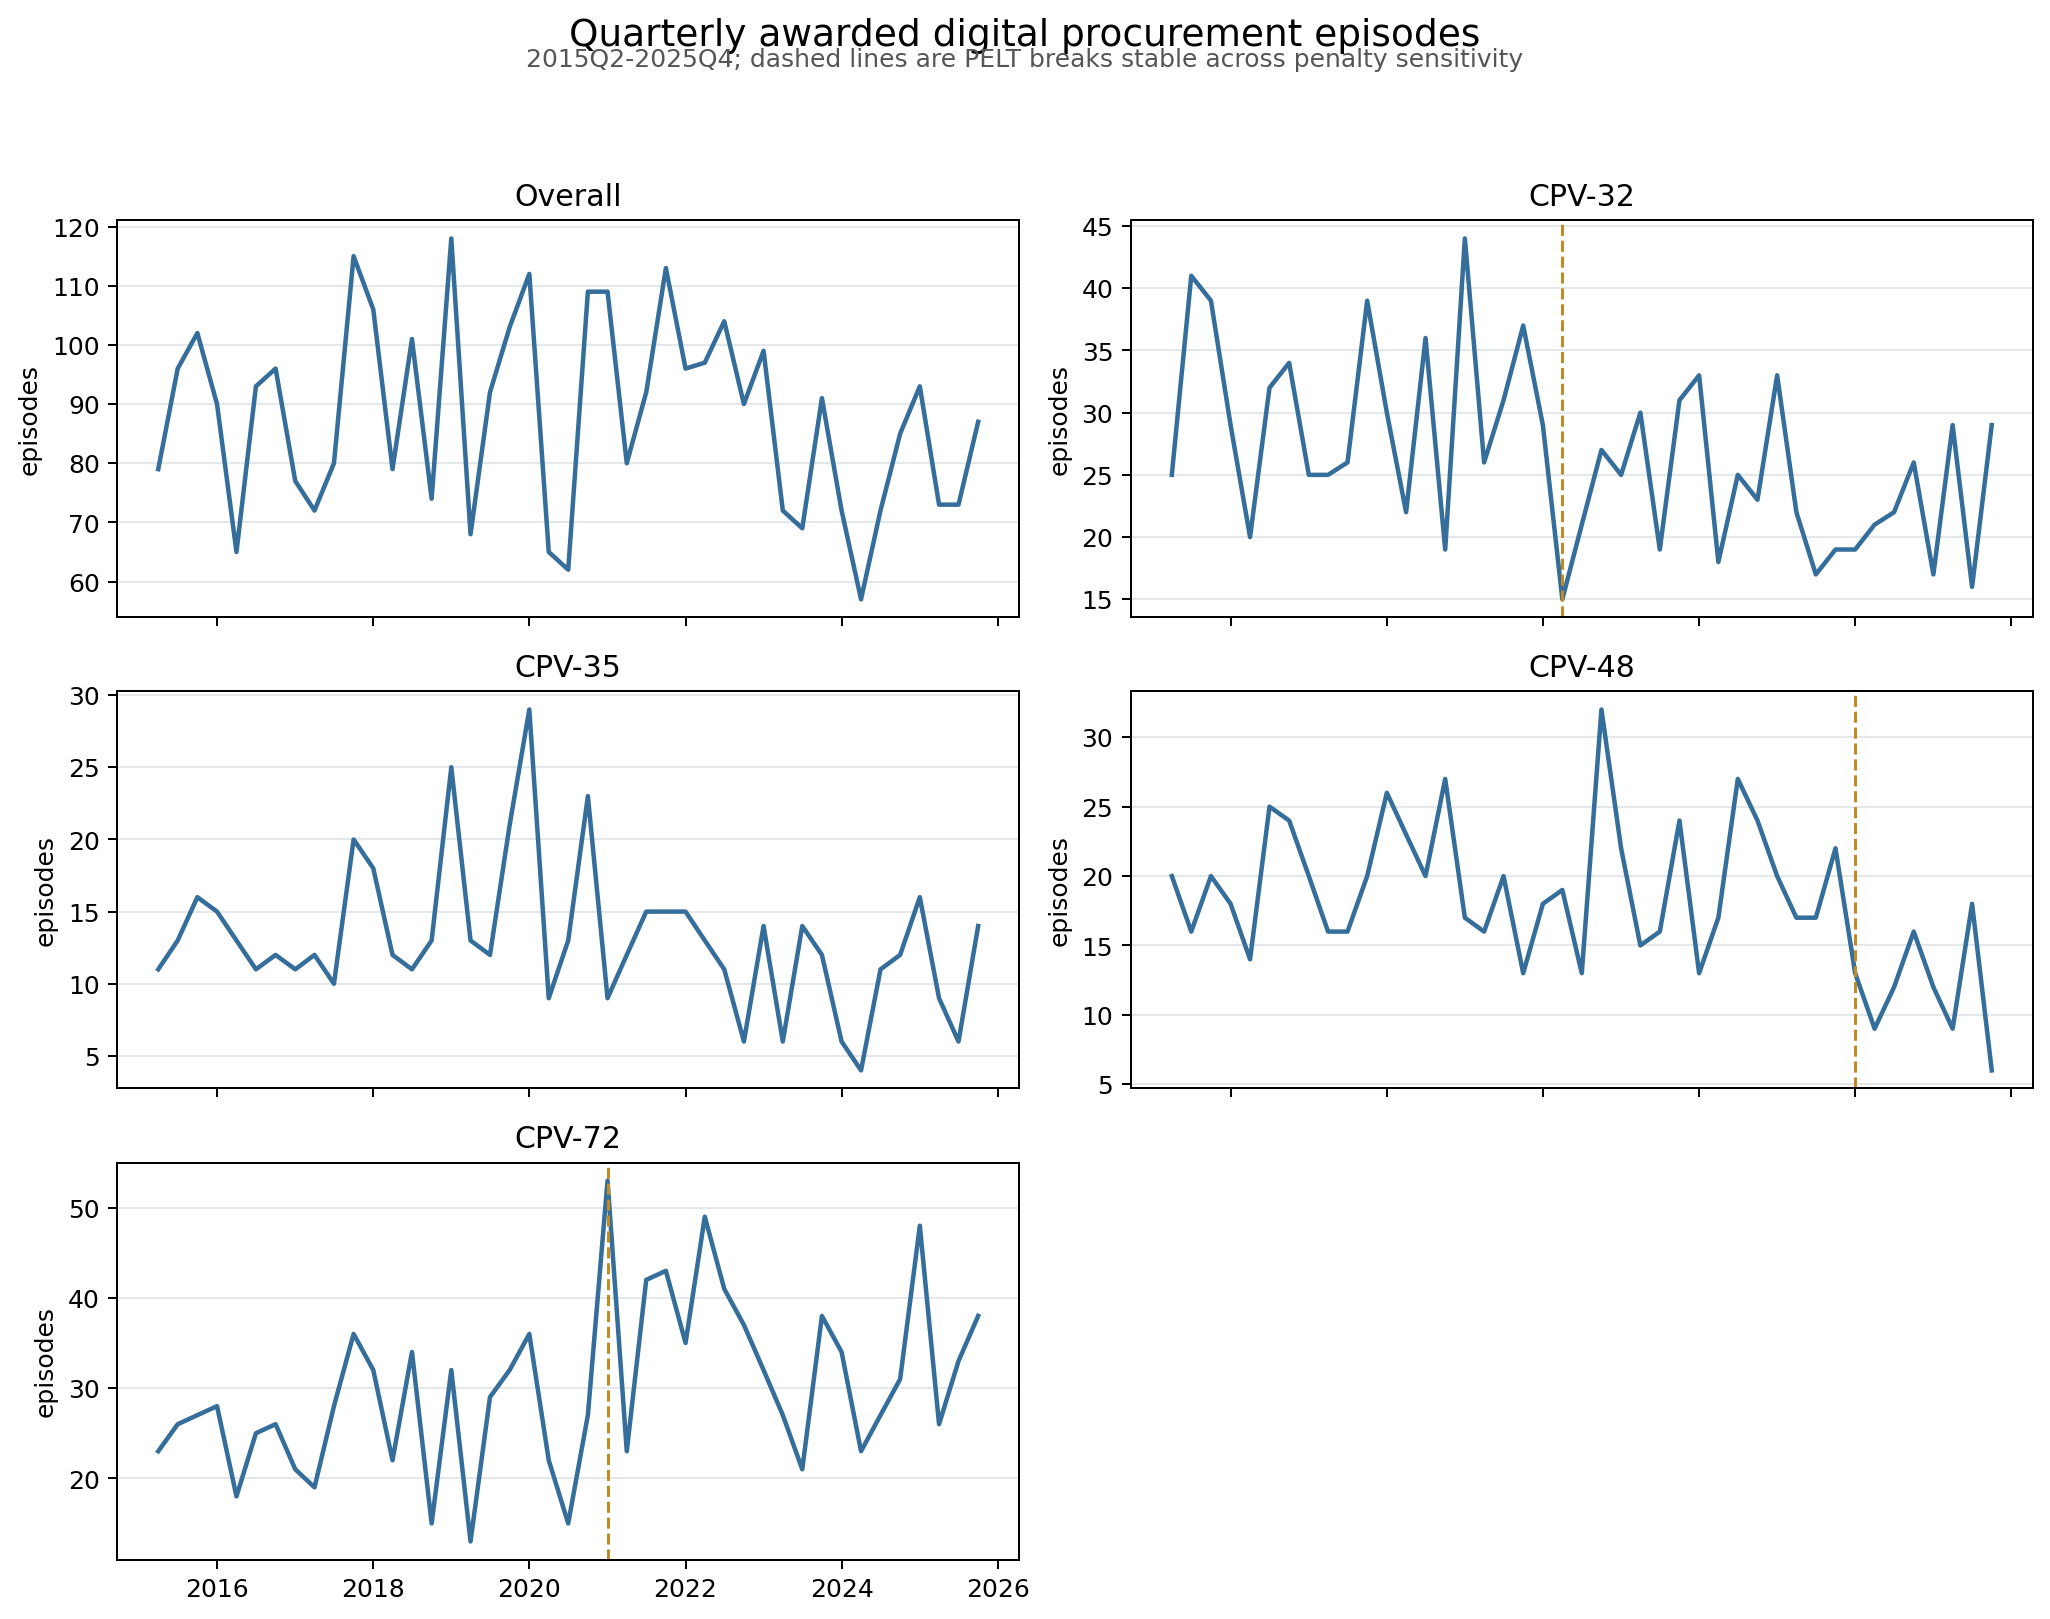
\includegraphics[width=0.95\linewidth]{figures/appF_quarterly_counts.png}
\caption{Quarterly awarded-episode counts, overall and by CPV division. The visual impression of movement in
individual segments is what the slope tests and the multiplicity correction are there to discipline: none of
these series carries a trend that survives correction for the five tests run together.}
\label{fig:appf-quarterly}
\end{figure}

\begin{figure}[htbp]
\centering
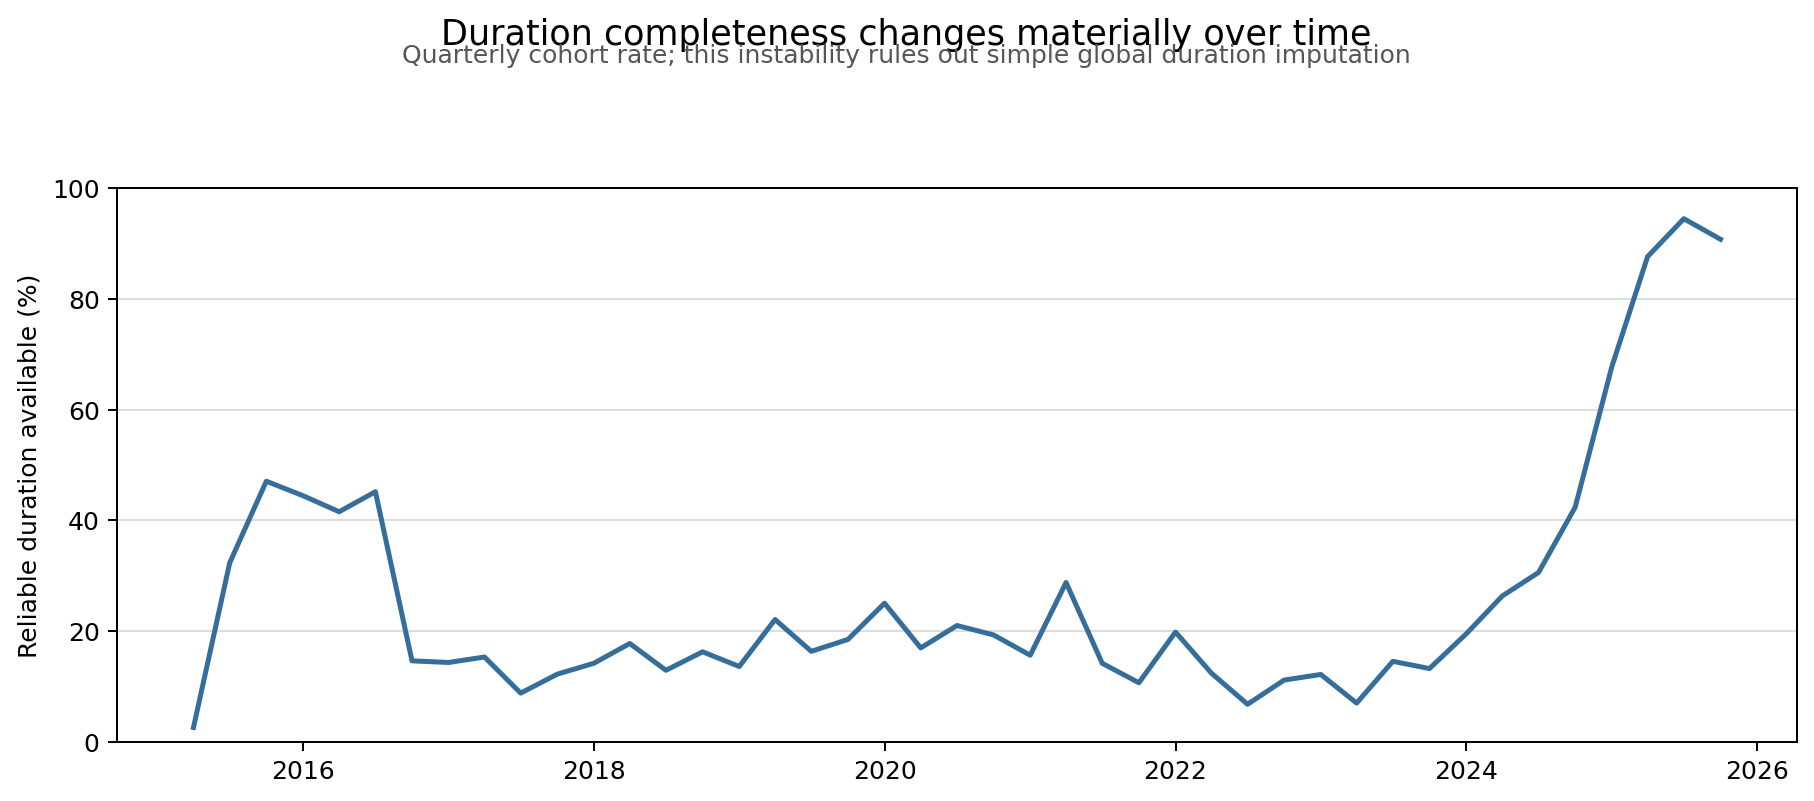
\includegraphics[width=0.78\linewidth]{figures/appF_duration_completeness.png}
\caption{Completeness of the declared-duration field by year. The sharp rise in 2025 is a schema and
completeness change, not evidence that contract durations changed. Median-duration trend claims would mix
periods with substantially different observation processes, which is why no change-point detection is run on
duration values.}
\label{fig:appf-duration}
\end{figure}

\section{Reproducibility}
\label{app:repro}

\subsection*{One command}

From the repository root:

\begin{quote}
\texttt{PYTHONPATH=. python3 scripts/run\_final\_pipeline.py}\\ \texttt{\phantom{xx}--with-notebooks --with-tests}
\end{quote}

The run executes every stage in dependency order:

\begin{quote}
\texttt{base $\rightarrow$ episodes $\rightarrow$ cohort $\rightarrow$ linkage}\\
\texttt{survival $\rightarrow$ technology $\rightarrow$ evidence and reader-artifact refresh}\\
\texttt{canonical state validation $\rightarrow$ manifest}
\end{quote}

The ordering is an invariant, not a convenience: every stage that writes an artifact runs before every stage
that reads it. The technology layer in particular runs \emph{before} the documents that quote its numbers and
before the validation gate, because the reverse order fails silently --- it republishes the previous run's
figures and certifies a state that is then overwritten.

\subsection*{Environment recorded with the run}

Python 3.12.6; pandas 2.3.3; numpy 2.4.4; scipy 1.17.1; scikit-learn 1.9.0; lifelines 0.30.3; statsmodels
0.14.6; ruptures 1.1.10; hmmlearn 0.3.3; joblib 1.5.3; matplotlib 3.10.9; pyarrow 25.0.1.

\subsection*{Canonical facts asserted by the manifest}

\begin{longtable}[]{@{}lr@{}}
\toprule\noalign{}
Fact & Value \\
\midrule\noalign{}
\endhead
Cohort rows & 3,800 \\
Events / censored & 544 / 3,256 \\
Event rate & 0.1432 \\
Selected linkage method & \texttt{M\_B\_text\_ranking} @ 70.0 \\
Technology specification & \texttt{M2\_tfidf\_logreg\_balanced} \\
Technology out-of-fold macro-F1 & 0.7442 \\
Calibration adopted & false (deployed variant: \texttt{raw}) \\
Episodes carrying a technology prediction & 3,800 \\
Canonical state validation & passed \\
\bottomrule\noalign{}
\end{longtable}

The manifest also records the git commit and working-tree state, and SHA-256 digests of the reference inputs
and canonical outputs, so a later run can be shown to have consumed the same inputs.

\subsection*{Cross-artifact validation gate}

\texttt{canonical\_state\_validation.json} runs fifteen checks across artifacts that are produced by different
stages, and the build fails if any returns false. They include: the accepted-link count agrees between the
linkage application and the survival events; accepted links are unique and contain no self-links; the
evaluations use the regional reference and its anchor counts match the reference manifest; no materialised
metadata points at a legacy path; the retired France-level benchmark and the duration-conditioned linkage arm
are absent from the repository; every cohort episode carries exactly one technology prediction; and the
deployed confidence variant is consistent across the configuration, the prediction file, the report, the
notebook and the run log.

That last check exists because of a defect it was written to prevent: an earlier version of the report
described a calibrated confidence score while the deployed artifact carried the raw one. Thirty technology
tests existed and none caught it, because the gap was between a \emph{document} and a \emph{configuration}
rather than inside the code.

\subsection*{Tests}

Thirteen test modules under \texttt{tests/}, collected by \texttt{pytest.ini}, which restricts collection to
that directory: pipeline structure, canonical layout, candidate-generation audit, evidence construction,
Fellegi--Sunter scoring, linkage rules, quality evidence, reference metrics, regional benchmark, review audit,
survival evidence, technology taxonomy, and the final pipeline. Passing tests establish implementation
consistency; they do not establish real-world linkage accuracy, and the report does not treat them as if they
did.

\subsection*{Where the numbers in this report live}

\begin{longtable}[]{@{}>{\raggedright\arraybackslash}p{5.6cm}>{\raggedright\arraybackslash}p{8.4cm}@{}}
\toprule\noalign{}
Content & Artifact \\
\midrule\noalign{}
\endhead
Cohort and selection funnel & survival\_cohort\_summary.json \\
Survival headline and diagnostics & survival\_analysis\_summary.json \\
Kaplan--Meier horizons & survival\_km\_horizons.csv \\
Cox estimates & survival\_cox\_results.csv \\
PH diagnostics & survival\_ph\_diagnostics.csv \\
Parametric comparison & survival\_parametric\_comparison.csv \\
Sensitivity arms & survival\_linkage\_sensitivity.csv \\
Borderline and template-risk checks & survival\_borderline\_link\_sensitivity.csv, survival\_template\_risk\_sensitivity.csv \\
Detectability & survival\_selection\_diagnostic.csv, survival\_cox\_detectability\_sensitivity.csv \\
Linkage evaluation & linkage\_evaluation\_validation.json, quality\_evidence/ \\
Candidate-generation audit & candidate\_generation\_audit.json \\
Technology model and deployment & technology/ (config, out-of-fold predictions, per-class metrics) \\
Trend series and signals & trend\_quarterly.csv, trend\_signal\_matrix.csv, trend\_breakpoints.csv \\
\bottomrule\noalign{}
\end{longtable}

All paths are relative to \texttt{data/processed/boamp/}.


\clearpage
\begin{otherlanguage}{french}
\section*{Note de synthèse (français)}
\addcontentsline{toc}{section}{Note de synthèse (français)}
\markboth{Note de synthèse}{}

\emph{Cette note est indépendante du rapport et se lit seule. Elle s'adresse à un lecteur non spécialiste.}

\textbf{\studentName{} --- ENSAE 2\textsuperscript{e} année --- Stage d'application 2025-2026}\\
\textbf{Gigalis --- Analyse et modélisation des marchés publics numériques à partir des données du BOAMP}

\subsection*{Le contexte}

Gigalis est le groupement d'intérêt public du numérique en Pays de la Loire. Il agit notamment comme centrale d'achat : il négocie des contrats mutualisés --- cloud, cybersécurité, réseaux, intelligence artificielle --- que les collectivités et établissements publics peuvent utiliser sans y être tenus. L'intérêt de ces contrats dépend du moment où ils sont ouverts. Trop tôt, ils restent inutilisés ; trop tard, les acheteurs ont déjà passé leurs propres marchés. D'où la question posée au stage : peut-on anticiper, à partir des données publiques, quand un besoin d'achat numérique va réapparaître ?

\subsection*{Ce que nous savons}

Les avis de marchés publics sont publiés au BOAMP, un bulletin officiel accessible librement. Le stage a traité \textbf{1,6 million d'avis} publiés entre 2015 et 2025, et en a tiré une population d'étude de \textbf{3 800 épisodes de commande publique attribués et reconstruits}, contenant un code CPV numérique, dans le Grand Ouest.

Un obstacle est apparu d'emblée, et il a structuré tout le travail : \textbf{le BOAMP n'indique jamais qu'un marché en renouvelle un autre}. Il n'existe donc aucune liste de renouvellements à partir de laquelle apprendre. Il a fallu construire l'information : pour chaque marché attribué, rechercher parmi les marchés publiés ensuite par le même acheteur celui qui poursuit le même besoin, et n'accepter ce rapprochement que lorsque la ressemblance est forte. Ce que l'étude mesure est donc un \textbf{`` successeur observable ''} --- un marché ultérieur qui prend visiblement le relais --- et non un renouvellement juridique. La distinction est maintenue partout, parce qu'elle change ce que l'on a le droit de conclure.

\subsection*{Ce que les modèles indiquent}

Sur cette base, environ \textbf{un épisode sur sept} voit apparaître un successeur observable avant fin 2025. La probabilité qu'un successeur devienne visible est estimée à \textbf{4,6 \% dans les douze mois} suivant l'attribution et \textbf{6,7 \% dans les vingt-quatre mois}. Le suivi diffère selon l'année d'attribution et l'estimateur de Kaplan--Meier prend explicitement en compte la censure à droite ; aucune explication causale n'est donnée au niveau numérique de ces probabilités.

Le résultat le plus utile n'est pas ce niveau moyen, mais son profil dans le temps : la probabilité \textbf{s'élève nettement entre la troisième et la quatrième année} du marché, ce qui correspond à la durée usuelle des contrats-cadres publics. C'est la fenêtre où la surveillance a le plus de valeur.

Deux comparaisons demandent des niveaux de prudence différents. Dans la population du Grand Ouest, les épisodes relevant du \textbf{CPV-35, matériel de sécurité et de surveillance} montrent un successeur observable plus tôt ; l'écart s'atténue lorsque l'on compare les achats d'un même acheteur. Les \textbf{accords-cadres} montrent également un successeur plus tôt. L'association reste positive après ajustement direct de la détectabilité et dans l'analyse principale intra-acheteur, mais son ampleur diminue.

Le second apport est d'une autre nature. Les marchés publics sont classés par une nomenclature administrative européenne, trop large pour un usage métier : une même catégorie mélange téléphonie, logiciels et prestations informatiques. Un modèle entraîné sur \textbf{500 avis annotés à la main} apprend à retrouver, à partir du seul texte de l'objet du marché, une segmentation métier en huit familles --- cloud, cybersécurité, réseaux, infrastructures, logiciels métier, données, intelligence artificielle, services informatiques. Il est \textbf{nettement meilleur que la nomenclature officielle} pour cet usage, et l'écart est mesuré avec sa marge d'incertitude. Gigalis dispose donc d'une lecture par technologie qui n'existait pas dans les données de départ.

\subsection*{Ce qui reste incertain}

Trois points doivent être dits clairement.

\textbf{La qualité des rapprochements n'est pas validée de façon indépendante.} Elle a été mesurée sur un échantillon de référence constitué pour le projet, et sur un très petit nombre de liens acceptés. L'ordre de grandeur est encourageant, l'intervalle d'incertitude est large. Une relecture par un spécialiste de la commande publique est le contrôle qui manque ; le protocole et l'échantillon sont prêts.

\textbf{Les niveaux absolus dépendent fortement de la règle choisie.} Selon que l'on est plus ou moins exigeant sur le rapprochement, le nombre de successeurs identifiés varie de 296 à 1 332. Plusieurs comparaisons résistent mieux aux changements de définition de l'événement, mais la composition par acheteur compte : le contraste CPV-35 s'atténue au sein d'un même acheteur, l'association des accords-cadres diminue sous contrôle, et le ralentissement CPV-48 apparaît surtout dans une analyse de sensibilité intra-acheteur.

\textbf{La prédiction marché par marché n'est pas établie.} Un modèle a été entraîné sur les années anciennes puis testé sur les années récentes sans réajustement : son estimation ponctuelle est proche du hasard et la validation temporelle disponible ne démontre pas une discrimination individuelle utile. Le modèle n'est donc pas utilisé comme moteur de classement individuel, et la liste des `` vingt marchés les plus susceptibles d'être renouvelés '' prévue au départ n'a pas été livrée.

\subsection*{Ce que cela signifie pour Gigalis}

Le travail fournit \textbf{un instrument de mesure et de veille, pas un moteur de prédiction}.

Concrètement, il permet de dire quels \emph{groupes} de marchés entrent dans la période où un successeur devient probable --- par segment et par ancienneté --- et de concentrer l'attention humaine sur la fenêtre de trois à quatre ans, en priorité sur les segments les plus rapides. Il fournit une segmentation technologique du portefeuille régional utilisable pour cartographier l'activité. Et il laisse un pipeline reproductible, documenté et testé, qui peut être relancé sur des données actualisées.

Il ne permet pas, en l'état, d'affirmer qu'un marché précis sera renouvelé, ni de prévoir l'évolution d'un segment : sur la période observée, aucune tendance de volume ne résiste aux tests statistiques appropriés.

\subsection*{Ce que nous recommandons ensuite}

\begin{enumerate}
\def\labelenumi{\arabic{enumi}.}
\tightlist
\item
  Faire relire un échantillon de rapprochements par un spécialiste indépendant, avant toute communication chiffrée sur la précision de la méthode.
\item
  Faire annoter une partie du corpus technologique par une seconde personne, afin de mesurer la fiabilité des étiquettes.
\item
  Fournir les données internes d'adhésion à Gigalis pour traiter la question causale --- l'ouverture d'un contrat mutualisé change-t-elle réellement le comportement d'achat des membres ? --- que les données publiques seules ne permettent pas d'aborder.
\item
  Traiter la prédiction individuelle comme une expérience distincte, avec ses variables, son protocole de validation et son critère de réussite fixés à l'avance, plutôt que comme un ajustement du modèle actuel.
\end{enumerate}

\end{otherlanguage}


\end{document}
